% Choose the language of your thesis passing 'french' or 'english' as
% \documentclass option.
% Note1: The 'page de garde' will always be written in French.
% Note2: You will have an error if you change the language of the document and
%        compile it without cleaning the auxiliary files. Compiling it again
%        should solve the problem.
\documentclass[french, a4paper, 11pt, twoside, pdftex]{StyleThese}

\newcommand{\included}{}
%\overfullrule=.5cm %% GROS TRAIT NOIR quand ça dépasse de la marge !

\usepackage{iflang}
\usepackage{bibentry}



%\usepackage[sectionbib]{chapterbib}          % Cross-reference package (Natural BiB)
%\usepackage{natbib}                  % Put References at the end of each chapter
%\usepackage{bibunits}
% Do not put 'sectionbib' option here.
% Sectionbib option in 'natbib' will do.


\usepackage{fancyhdr}                    % Fancy Header and Footer

\usepackage[utf8]{inputenc}
\usepackage[T1]{fontenc}
\usepackage[french]{babel} %
\usepackage{lmodern} \normalfont %to load T1lmr.fd 
\DeclareFontShape{T1}{cmr}{b}{sc} { <-> ssub * cmr/bx/sc }{}
%\hyphenation{gar}

\usepackage{amsmath,amssymb}             % AMS Math
\usepackage{nicefrac}
\usepackage{siunitx}					%% Unites Math SI

\usepackage{blindtext}

\usepackage{datetime}

\usepackage{lipsum} 

\usepackage[inline]{enumitem}

\usepackage{hhline}
%\usepackage[left=1.5in,right=1.3in,top=1.1in,bottom=1.1in]{geometry}
\usepackage[left=1.5in,right=1.3in,top=1.1in,bottom=1.1in,includefoot,includehead,headheight=13.6pt]{geometry}

%%\renewcommand{\baselinestretch}{1.05}

%%%%%%%% Multi-figures avec sub-captions
\usepackage{caption}
\usepackage{subcaption}

% Table of contents for each chapter

\usepackage[nottoc, notlof, notlot]{tocbibind}
\usepackage[nohints]{minitoc}
\setcounter{minitocdepth}{2}
\mtcindent=15pt
% Use \minitoc where to put a table of contents

\usepackage{aecompl}

%% Package cosmetic meilleur layout du texte en jouant sur le spacing par caractères
\usepackage[activate={true,nocompatibility},final,tracking=true,kerning=true,factor=1100,stretch=10,shrink=10]{microtype}
\usepackage[absolute,overlay]{textpos} 
\setlength{\TPHorizModule}{\paperwidth}\setlength{\TPVertModule}{\paperheight}
\sloppy

%%%%%%%%%%% JOLIS TABLEAUX
\usepackage{tabularx}		%\usepackage{tabular}
\usepackage{longtable}
\usepackage{multirow}
\newcommand{\mc}{\multicolumn} 
\newcommand{\mr}[2]{\multirow{#1}{*}{#2}} 	\newcommand{\mrQ}{\multirow{-4}{*}}
\usepackage{booktabs}

\usepackage[usenames,dvipsnames]{xcolor} 

\makeatletter
\newcommand{\ccolor}[3][]{%
	\kern-\fboxsep
	\if\relax\detokenize{#1}\relax
	\expandafter\@firstoftwo
	\else
	\expandafter\@secondoftwo
	\fi
	{\colorbox{#2}}%
	{\colorbox[#1]{#2}}%
	{#3}\kern-\fboxsep
}
\makeatother

%%%%% Insertion graphiques format PGF
\usepackage{pgfplots}
\pgfplotsset{width=\linewidth, compat=1.16}%, compat=1.17}
\usepackage{adjustbox}          %%% PERMET DE LES RECADRER + FACILEMENT


%%%%%%%%%% Bullets de listes sans saut de ligne %%%%%%%%%%
\usepackage{xparse}

\ExplSyntaxOn%
\seq_new:N \l_local_enum_seq

\newcommand{\storethestuff}[1]{%
  \seq_set_from_clist:Nn \l_local_enum_seq {#1}%
}

\newcommand{\dotheenumstuff}{%
\int_zero:N \l_tmpa_int
\seq_map_inline:Nn \l_local_enum_seq {%
    \int_incr:N \l_tmpa_int% Increase the counter
    \item ##1
    % Check whether the list has reached the end -- if so, use '.' instead of ','
    %\int_compare:nNnTF 
    % { \l_tmpa_int } < {\seq_count:N \l_local_enum_seq} 
    % {,} {.}
  }
}
\ExplSyntaxOff

\NewDocumentCommand{\linebullets}{+m}{%
  \storethestuff{#1}%
  \begin{enumerate*}[label={\alph*)},font={\bfseries},itemjoin={{, }}]
    \dotheenumstuff%
  \end{enumerate*}
}

\newcommand{\cmnt}[1]{}  %%%%% AJOUT DE COMMENTAIRE MULTILIGNES


%%%%%%%%%% ECRITURE CARACTERES DANS UN CERCLE %%%%%%%%%%
%\def\circleTxt[#1]{\raisebox{.5pt}{\textcircled{\raisebox{-1pt}{#1}}}}
\newcommand{\ctxt}[1]{\raisebox{.5pt}{\textcircled{\raisebox{-1.2pt}{#1}}}}
% Glossary / list of abbreviations

\usepackage[intoc]{nomencl}
\IfLanguageName{english}{%
\renewcommand{\nomname}{Glossary}
}{ %
\renewcommand{\nomname}{Liste des Abréviations}
}

\makenomenclature

% My pdf code

\usepackage{ifpdf}

\ifpdf
  \usepackage[pdftex]{graphicx}
  \DeclareGraphicsExtensions{.pdf,PDF,.png,PNG,.jpg,JPG}
  \usepackage[pagebackref,hyperindex=true]{hyperref} %% use \autoref{} instead of Table~\ref{}.
  \usepackage{tikz}
  \usetikzlibrary{arrows,shapes,calc}
\else
  \usepackage{graphicx}
  \DeclareGraphicsExtensions{.ps,.eps}
  \usepackage[a4paper,dvipdfm,pagebackref,hyperindex=true]{hyperref}
\fi

\graphicspath{{.}{schemas/}{graphiques/}{tables/}}

%% nicer backref links. NOTE: The flag ThesisInEnglish is used to define the
% language in the back references. Read more about it in These.tex

\IfLanguageName{english}{
\renewcommand*{\backref}[1]{}
\renewcommand*{\backrefalt}[4]{%
\ifcase #1 %
(Not cited.)%
\or
(Cited in page~#2.)%
\else
(Cited in pages~#2.)%
\fi}
\renewcommand*{\backrefsep}{, }
\renewcommand*{\backreftwosep}{ and~}
\renewcommand*{\backreflastsep}{ and~}
}{
\renewcommand*{\backref}[1]{}
\renewcommand*{\backrefalt}[4]{%
\ifcase #1 %
(Non cité.)%
\or
(Cité en page~#2.)%
\else
(Cité en pages~#2.)%
\fi}
\renewcommand*{\backrefsep}{, }
\renewcommand*{\backreftwosep}{ et~}
\renewcommand*{\backreflastsep}{ et~}
}

% Links in pdf
\usepackage{color}
\definecolor{linkcol}{rgb}{0,0,0.4} 
\definecolor{citecol}{rgb}{0.5,0,0} 
\definecolor{linkcol}{rgb}{0,0,0} 
\definecolor{citecol}{rgb}{0,0,0}
% Change this to change the informations included in the pdf file

\hypersetup
{
bookmarksopen=true,
pdftitle="Prévention des fautes temporelles sur architectures multicœur pour les systèmes à criticité mixte",
pdfauthor="Daniel LOCHE", %auteur du document
pdfsubject="Thèse", %sujet du document
%pdftoolbar=false, %barre d'outils non visible
pdfmenubar=true, %barre de menu visible
pdfhighlight=/O, %effet d'un clic sur un lien hypertexte
colorlinks=true, %couleurs sur les liens hypertextes
pdfpagemode=UseNone, %aucun mode de page
%pdfpagelayout=DoublePage, %ouverture en simple page
pdffitwindow=true, %pages ouvertes entierement dans toute la fenetre
linkcolor=linkcol, %couleur des liens hypertextes internes
citecolor=citecol, %couleur des liens pour les citations
urlcolor=linkcol %couleur des liens pour les url
}

% definitions.
% -------------------

\setcounter{secnumdepth}{3}
\setcounter{tocdepth}{2}

% Some useful commands and shortcut for maths:  partial derivative and stuff

\newcommand{\pd}[2]{\frac{\partial #1}{\partial #2}}
\def\abs{\operatorname{abs}}
\def\argmax{\operatornamewithlimits{arg\,max}}
\def\argmin{\operatornamewithlimits{arg\,min}}
\def\diag{\operatorname{Diag}}
\newcommand{\eqRef}[1]{(\ref{#1})}
\newcommand{\nline}{\smallbreak\noindent}

\usepackage{rotating}                    % Sideways of figures & tables

% \usepackage{txfonts}                     % Public Times New Roman text & math font
  
%%% Fancy Header %%%%%%%%%%%%%%%%%%%%%%%%%%%%%%%%%%%%%%%%%%%%%%%%%%%%%%%%%%%%%%%%%%
% Fancy Header Style Options

\pagestyle{fancy}                       % Sets fancy header and footer
\fancyfoot{}                            % Delete current footer settings

%\renewcommand{\chaptermark}[1]{         % Lower Case Chapter marker style
%  \markboth{\chaptername\ \thechapter.\ #1}}{}} %

%\renewcommand{\sectionmark}[1]{         % Lower case Section marker style
%  \markright{\thesection.\ #1}}         %

\fancyhead[LE,RO]{\bfseries\thepage}    % Page number (boldface) in left on even
% pages and right on odd pages
\fancyhead[RE]{\bfseries\nouppercase{\leftmark}}      % Chapter in the right on even pages
\fancyhead[LO]{\bfseries\nouppercase{\rightmark}}     % Section in the left on odd pages

\let\headruleORIG\headrule
\renewcommand{\headrule}{\color{black} \headruleORIG}
\renewcommand{\headrulewidth}{1.0pt}
\usepackage{colortbl}
\arrayrulecolor{black}

\fancypagestyle{plain}{
  \fancyhead{}
  \fancyfoot{}
  \renewcommand{\headrulewidth}{0pt} %%%%%%%%%%%%%%%%%%%%%%%%%%%%%%%%%%%%%%%%%%%%%%%%%%%%%%%%%%%%%%%%%%%%%%%%%%%%%%%%%%%%%
}

%\usepackage{MyAlgorithm}
%\usepackage[noend]{MyAlgorithmic}
%\usepackage[ED=EDSYS-SystEmb, Ets=INP]{tlsflyleaf}

%%% Clear Header %%%%%%%%%%%%%%%%%%%%%%%%%%%%%%%%%%%%%%%%%%%%%%%%%%%%%%%%%%%%%%%%%%
% Clear Header Style on the Last Empty Odd pages
\makeatletter

\def\cleardoublepage{\clearpage\if@twoside \ifodd\c@page\else%
  \hbox{}%
  \thispagestyle{empty}%              % Empty header styles
  \newpage%
  \if@twocolumn\hbox{}\newpage\fi\fi\fi}

\makeatother
 
%%%%%%%%%%%%%%%%%%%%%%%%%%%%%%%%%%%%%%%%%%%%%%%%%%%%%%%%%%%%%%%%%%%%%%%%%%%%%%% 
% Prints your review date and 'Draft Version' (From Josullvn, CS, CMU)
\newcommand{\reviewtimetoday}[2]{\special{!userdict begin
    /bop-hook{gsave 20 710 translate 45 rotate 0.8 setgray
      /Times-Roman findfont 12 scalefont setfont 0 0   moveto (#1) show
      0 -12 moveto (#2) show grestore}def end}}
% You can turn on or off this option.
% \reviewtimetoday{\today}{Draft Version}
%%%%%%%%%%%%%%%%%%%%%%%%%%%%%%%%%%%%%%%%%%%%%%%%%%%%%%%%%%%%%%%%%%%%%%%%%%%%%%% 

\newenvironment{maxime}[1]
{
	\def\Arg{#1}
\vspace*{0cm}
\hfill
\begin{minipage}{0.6\textwidth}%
%\rule[0.5ex]{\textwidth}{0.1mm}\\%
\hrulefill $\:$ \\%$\:$ {\bf #1}\\
%\vspace*{-0.25cm}
\it 
}%
{%
	
\hrulefill $\:$ {\bf \Arg}
\vspace*{0.5cm}%
\end{minipage}
}

\let\minitocORIG\minitoc
\renewcommand{\minitoc}{\minitocORIG \vspace{1.5em}}

%\usepackage{slashbox}

\newenvironment{bulletList}%
{ \begin{list}%
	{$\bullet$}%
	{\setlength{\labelwidth}{25pt}%
	 \setlength{\leftmargin}{30pt}%
	 \setlength{\itemsep}{\parsep}}}%
{ \end{list} }


%%%%%%% Outils pour \comment \alert \add %%%%%
\usepackage{easyReview}
\usepackage{soulutf8} % for accented letters

\let\newalert\alert
\renewcommand{\alert}[1]{\textit{\newalert{#1}}}

%\usepackage[commandnameprefix=ifneeded]{changes} %% \chhighlight and \chcomment to avoid collision with easyReview
\renewcommand{\epsilon}{\varepsilon}

% centered page environment

\newenvironment{vcenterpage}
{\newpage\vspace*{\fill}\thispagestyle{empty}\renewcommand{\headrulewidth}{0pt}}
{\vspace*{\fill}}

\usepackage{tablefootnote}

%%%%%% MISE EN FORME CADRES DEFINITIONS/THEOREMES/LEMES %%%%%%%%%%
\usepackage{amsthm}  % for theoremstyle

\theoremstyle{plain} 
\newtheorem{theorem}{Théorème}[section]
\newtheorem{corollary}{Corolaire}[theorem]

%\theoremstyle{lemma}
%\newtheorem{lemma}[theorem]{Lemme}


\theoremstyle{definition}
\newtheorem{definition}[theorem]{Définition}


\cmnt{
	\usepackage{ntheorem} %\usepackage{amsthm}  % for theoremstyle
	%\usepackage{mdframed}
	\usepackage[most]{tcolorbox}
	
	\theoremstyle{plain} 
	\theoremindent20pt
	\theoremheaderfont{\normalfont\bfseries\hspace{-\theoremindent}}
	\newtheorem{theorem}{Théorème}[section]
	\newtheorem{corollary}{Corolaire}[theorem]
	
	\theoremstyle{plain}
	\newtheorem{lemma}[theorem]{Lemme}
	
	
	\tcolorboxenvironment{theorem}{
		blanker,
		breakable,
		before skip=\topsep,
		after skip=\topsep,
		borderline west={1pt}{10pt}{double, shorten <=12pt}
	}
	
	\theorembodyfont{\normalfont}
	\theoremindent20pt
	\theoremheaderfont{\normalfont\bfseries\hspace{-\theoremindent}}
	\newtheorem{definition}[theorem]{Définition}
	
	
	\tcolorboxenvironment{definition}{
		blanker,
		breakable,
		before skip=\topsep,
		after skip=\topsep,
		borderline west={1pt}{10pt}{shorten <=12pt}
	}
}

\cmnt{ 
	\begin{theorem}
		Ceci est un Théorème.
	\end{theorem} 
	
	\begin{corollary}
		Ceci est un Corollaire.
	\end{corollary}
	
	\begin{definition}
		Ceci est une Définition.
	\end{definition}
	
	\begin{lemma}
		Ceci est un Lemme.
	\end{lemma}
}

\def\UrlBigBreaks{\do\/\do-\do:}
\usepackage{url}


\renewcommand\nomgroup[1]{%  % GROUPEMENT DES ÉLÉMENTS DE LA NOMENCLATURE. ON PEUT EN AJOUTER AUTANT QUE NÉCESSAIRE.
	\item[\bfseries
	\ifstrequal{#1}{D}{Abréviations}{%
		\ifstrequal{#1}{A}{Modèle de Tâches}{%
			\ifstrequal{#1}{B}{Modèle de Chaîne de tâches}{%
				\ifstrequal{#1}{C}{Mécanisme de Surveillance et Contrôle}{%
		}}}}%
		]
	}
\setlength{\nomlabelwidth}{2cm}			%% PARAMÉTRABLE POUR ADAPTER LE PLACEMENT DES COLONNES DE LA NOMENCLATURE, SELON LA LONGUEUR DE VOTRE ABRÉVIATION LA PLUS LONGUE

%% Copyright 2013 Tristan GREGOIRE
%% Copyright 2015 Yann BACHY
%
% This work may be distributed and/or modified under the
% conditions of the LaTeX Project Public License, either version 1.3
% of this license or (at your option) any later version.
% The latest version of this license is in
%   http://www.latex-project.org/lppl.txt
% and version 1.3 or later is part of all distributions of LaTeX
% version 2005/12/01 or later.
%
%
% This work has the LPPL maintenance status `maintained'.
% 
% The Current Maintainer of this work is T. GREGOIRE
%

%\documentclass{book}

% Loading the tlsflyleaf.sty package require some option to define the
% establishment name, the doctoral school and the PhD speciality.
% In that aim you have 2 key-value option:
%   - Ets=<value> : define the establishment name
%   - ED=<value>  : define the doctoral school and speciality
%   - ED2=<value> : define the second speciality ("double mention"). OPTIONAL.
% The full list of accepted values for each option could be find either
% in the documentation or in ED-list.txt and Ets-list.txt files provide with the package.
%\usepackage[ED=MITT - STICRT, Ets=INSA]{tlsflyleaf}
%\usepackage[ED=SDU2E-Ast, ED2=SDU2E-Eco, Ets=UT3]{tlsflyleaf}
\usepackage[ED=EDSYS-SystEmb, Ets=INP]{tlsflyleaf}

% ==================
% Setup basic string
% - PhD Title
% - author
% - defence date
% - laboratory
% - cotutelle
\title{Prévention des fautes temporelles sur architectures multicœur pour les systèmes à criticité mixte}
\author{Daniel LOCHE}
\defencedate{01/07/2022}
\lab{Laboratoire d'analyse et d'architecture des systèmes -- LAAS-CNRS}
%\cotutelle{}

% ==================
% Setup people like your boss, the jury team and the referees
% - First you need to define how number they will be in each category
%   It is done with the commands \nboss{n}, \nreferee{n} and \njudge{n}.
%   You can define more people in each category than the number given 
%   but only the first "\npeople" will be print.
% - Then use the command \makesomeone{<category>}{<number>}{<name>}{<status>}{<other>}
%   where:
%     <category> should be select in ['boss', 'referee', 'judge', 'invitee']
%     <number>   is the rank for printing the person. 
%                Only number <= "\npeople" will be printed
%     <name>     First name and last name of the people
%     <status>   Is (s)he a "charg\'e de recher" ou un "professeur d'universit\'e"...
%     <other>    What ever string you want to add (laboratory, jury member place...).
%% Boss
\nboss{2}
\makesomeone{boss}{2}{Michaël LAUER}{}{}  % Sera affiche en second
\makesomeone{boss}{1}{Jean-Charles FABRE}{}{} % Sera afiche en premier
%% Referee
\nreferee{2}
\makesomeone{referee}{1}{Liliana CUCU-GROSJEAN}{Chargée de Recherche}{INRIA, Paris}
\makesomeone{referee}{2}{Emmanuel GROLLEAU}{Professeur}{ISAE-ENSMA, Poitiers}
%% Judges
\njudge{7}
%\cmnt
\makesomeone{judge}{3}{Claire PAGETTI}{Ingénieure de Recherche, \\ONERA}{Examinatrice}
\makesomeone{judge}{5}{Jean-Charles FABRE}{Professeur des Universités, \\Toulouse INP}{Directeur de Thèse}
\makesomeone{judge}{4}{Sébastien FAUCOU}{Maître de Conférences, \\Univ. de Nantes}{Examinateur}
\makesomeone{judge}{6}{Michaël LAUER}{Maître de Conférences, \\Univ. Toulouse 3}{Co-directeur de Thèse}
\makesomeone{judge}{2}{Liliana CUCU-GROSJEAN}{Directrice de Recherche, \\INRIA}{Rapporteure}
\makesomeone{judge}{1}{Emmanuel GROLLEAU}{Professeur des Universités, \\ISAE-ENSMA}{Président}

\cmnt
{
\makesomeone{judge}{1}{Claire PAGETTI}{Ing. de Recherche\cmnt{, \\ONERA}}{Président du Jury}
\makesomeone{judge}{5}{Jean-Charles FABRE}{Professeur des Universités\cmnt{, \\Toulouse INP}}{Directeur de Thèse}
\makesomeone{judge}{2}{Sébastien FAUCOU}{Maître de Conférences\cmnt{, \\Univ. de Nantes}}{Examinateur}
\makesomeone{judge}{6}{Michael LAUER}{Maître de Conférences\cmnt{, \\Univ. Toulouse 3}}{Co-directeur de Thèse}
\makesomeone{judge}{4}{Liliana CUCU-GROSJEAN}{Directrice de Recherche\cmnt{, \\INRIA}}{Rapporteure}
\makesomeone{judge}{3}{Emmanuel GROLLEAU}{Professeur des Universités\cmnt{, \\ISAE-ENSMA}}{Rapporteur}
}
%% Invitees
%\ninvitee{1}
\makesomeone{judge}{7}{François GŒUSSE}{Ingénieur, Renault SWLabs}{Invité}

% ============================================================
% DOCUMENT
%\begin{document}
%    \makeflyleaf
%\end{document}


\begin{document}

\makeflyleaf
\cleardoublepage

\dominitoc

\pagenumbering{roman}

 \cleardoublepage
%%%%%%%%%%%%%%%%%%
 %%%%% MAXIME %%%%%
%\topskip-10cm
\vspace*{5cm}
% \begin{maxime}{Pierre-Henri Cami.}
%	Souvent une évolution est une révolution sans en avoir l'R.
%\end{maxime}
\epigraph{{\large Ceci est ma citation pour faire stylé}}
{{\smallbreak\large \textit{Moi-même}}}
%\vspace*{\fill}

\cleardoublepage

%Another use of \if toggle can be found at the end of this file.
\IfLanguageName{english}{%
\section*{Acknowledgments}
}{%
\section*{Préface}
\addstarredchapter{Préface}

	Remerciements, à écrire à la fin.

}


\tableofcontents
%\makenomenclature


 %%%%%%%%%%%%%%%%%%%%%%%%
{ %%%%% NOMENCLATURE %%%%%  [lettre, ordre]{contenu}
								% => lettre = groupe tel que défini plus haut.
								% => ordre = si différents, permet de forcer un ordre d'apparition (sinon, ordre alphébétique)
								% => contenu = bah ton contenu, andouille.
	\nomenclature[A, 01]{$\tau_i$}{Tâche, d'indice i}
	\nomenclature[A, 03]{$T_i$}{Période d'apparition d'une tâche}
	\nomenclature[A, 04]{$D_i$}{Date limite d'échéance à la terminaison d'une tâche}
	\nomenclature[A, 05]{$C_i$}{Temps d'exécution pire cas d'une tâche}
	\nomenclature[A, 06]{$L_i$}{Niveau de criticité d'une tâche}
	\nomenclature[A, 07]{$\tau_{i,j}$}{j\up{ème} occurrence d'exécution de la tâche $\tau_i$ à sa période $T_i$}
	\nomenclature[A, 08]{$a_{i,j}$}{Moment d'activation du job $\tau_{i,j}$}
	\nomenclature[A, 09]{$s_{i,j}$}{Début d'exécution du job $\tau_{i,j}$}
	\nomenclature[A, 10]{$e_{i,j}$}{Fin d'exécution (terminaison) du job $\tau_{i,j}$}
	\nomenclature[B, 20]{$succ(\tau_i)$}{Fonction qui permet de trouver le job successeur du job $\tau_i$ d'une chaîne de tâches}
	\nomenclature[B, 21]{$succ^p(\tau_i)$}{fonction itérative pour trouver le p\up{ème} successeur du job $\tau_i$}
	\nomenclature[B, 15]{$R_j$}{Temps de réponse bout-en-bout d'une chaîne de tâches}
	\nomenclature[B, 16]{$D_c$}{Délai limite d'échéance d'exécution bout-en-bout d'une chaîne de tâche}
	\nomenclature[B, 23]{$S(t)$}{Etat de la chaîne de tâches à l'instant $t$}
	\nomenclature[B, 24]{$ET(j,t)$}{j\up{ème} trace d'exécution de la chaîne de tâches, à un instant t}
	\nomenclature[B, 30]{$RT(t)$}{Temps de réponse partiel d'une chaîne de tâche active à l'instant t}
	\nomenclature[B, 31]{$rWCRT(t)$}{Pire Temps de Réponse Restant d'une chaîne de tâche}
	\nomenclature[C, 42]{$T_{CCC}$}{Période de fonctionnement du Core Control Component}
	\nomenclature[C, 43]{$W_{MAX}$}{Durée maximale garantie entre 2 points de surveillance}
	\nomenclature[C, 44]{$t_{SW}$}{Latence de changement de mode}
	\nomenclature[C, 40]{TWC}{Task-Wrapper Component : module d'encapsulation pour la surveillance des tâches}
	\nomenclature[C, 41]{CCC}{Core Control Component : module de décision de changement de mode}

}

\printnomenclature
\cmnt{	 %% IMPORTANT SI T'AS DES SOUCIS DE DÉCALLAGE ENTRE LES PLANS DANS CHAQUE CHAPITRE ET LE NUMÉRO DES CHAPITRES !!
% Use \mtcfixnomenclature below if you have a glossary (added with
% \printnomenclature above) and you're see a shift in the mini-table of
% contents at the begining of each chapter (example: no mini-toc in chapter 1;
% mini-toc of chapter 1 appearing in chapter 2; and so on).
%
% You should not use \mtcfixnomenclature if you have no glossary (that means,
% if you don't use \printnomenclature or if your glossary is empty).
}
\mtcfixnomenclature


\mainmatter

\ifdefined\included
\else
\documentclass[french, a4paper, 11pt, twoside, pdftex]{StyleThese}
\usepackage{iflang}
\usepackage{bibentry}



%\usepackage[sectionbib]{chapterbib}          % Cross-reference package (Natural BiB)
%\usepackage{natbib}                  % Put References at the end of each chapter
%\usepackage{bibunits}
% Do not put 'sectionbib' option here.
% Sectionbib option in 'natbib' will do.


\usepackage{fancyhdr}                    % Fancy Header and Footer

\usepackage[utf8]{inputenc}
\usepackage[T1]{fontenc}
\usepackage[french]{babel} %
\usepackage{lmodern} \normalfont %to load T1lmr.fd 
\DeclareFontShape{T1}{cmr}{b}{sc} { <-> ssub * cmr/bx/sc }{}
%\hyphenation{gar}

\usepackage{amsmath,amssymb}             % AMS Math
\usepackage{nicefrac}
\usepackage{siunitx}					%% Unites Math SI

\usepackage{blindtext}

\usepackage{datetime}

\usepackage{lipsum} 

\usepackage[inline]{enumitem}

\usepackage{hhline}
%\usepackage[left=1.5in,right=1.3in,top=1.1in,bottom=1.1in]{geometry}
\usepackage[left=1.5in,right=1.3in,top=1.1in,bottom=1.1in,includefoot,includehead,headheight=13.6pt]{geometry}

%%\renewcommand{\baselinestretch}{1.05}

%%%%%%%% Multi-figures avec sub-captions
\usepackage{caption}
\usepackage{subcaption}

% Table of contents for each chapter

\usepackage[nottoc, notlof, notlot]{tocbibind}
\usepackage[nohints]{minitoc}
\setcounter{minitocdepth}{2}
\mtcindent=15pt
% Use \minitoc where to put a table of contents

\usepackage{aecompl}

%% Package cosmetic meilleur layout du texte en jouant sur le spacing par caractères
\usepackage[activate={true,nocompatibility},final,tracking=true,kerning=true,factor=1100,stretch=10,shrink=10]{microtype}
\usepackage[absolute,overlay]{textpos} 
\setlength{\TPHorizModule}{\paperwidth}\setlength{\TPVertModule}{\paperheight}
\sloppy

%%%%%%%%%%% JOLIS TABLEAUX
\usepackage{tabularx}		%\usepackage{tabular}
\usepackage{longtable}
\usepackage{multirow}
\newcommand{\mc}{\multicolumn} 
\newcommand{\mr}[2]{\multirow{#1}{*}{#2}} 	\newcommand{\mrQ}{\multirow{-4}{*}}
\usepackage{booktabs}

\usepackage[usenames,dvipsnames]{xcolor} 

\makeatletter
\newcommand{\ccolor}[3][]{%
	\kern-\fboxsep
	\if\relax\detokenize{#1}\relax
	\expandafter\@firstoftwo
	\else
	\expandafter\@secondoftwo
	\fi
	{\colorbox{#2}}%
	{\colorbox[#1]{#2}}%
	{#3}\kern-\fboxsep
}
\makeatother

%%%%% Insertion graphiques format PGF
\usepackage{pgfplots}
\pgfplotsset{width=\linewidth, compat=1.16}%, compat=1.17}
\usepackage{adjustbox}          %%% PERMET DE LES RECADRER + FACILEMENT


%%%%%%%%%% Bullets de listes sans saut de ligne %%%%%%%%%%
\usepackage{xparse}

\ExplSyntaxOn%
\seq_new:N \l_local_enum_seq

\newcommand{\storethestuff}[1]{%
  \seq_set_from_clist:Nn \l_local_enum_seq {#1}%
}

\newcommand{\dotheenumstuff}{%
\int_zero:N \l_tmpa_int
\seq_map_inline:Nn \l_local_enum_seq {%
    \int_incr:N \l_tmpa_int% Increase the counter
    \item ##1
    % Check whether the list has reached the end -- if so, use '.' instead of ','
    %\int_compare:nNnTF 
    % { \l_tmpa_int } < {\seq_count:N \l_local_enum_seq} 
    % {,} {.}
  }
}
\ExplSyntaxOff

\NewDocumentCommand{\linebullets}{+m}{%
  \storethestuff{#1}%
  \begin{enumerate*}[label={\alph*)},font={\bfseries},itemjoin={{, }}]
    \dotheenumstuff%
  \end{enumerate*}
}

\newcommand{\cmnt}[1]{}  %%%%% AJOUT DE COMMENTAIRE MULTILIGNES


%%%%%%%%%% ECRITURE CARACTERES DANS UN CERCLE %%%%%%%%%%
%\def\circleTxt[#1]{\raisebox{.5pt}{\textcircled{\raisebox{-1pt}{#1}}}}
\newcommand{\ctxt}[1]{\raisebox{.5pt}{\textcircled{\raisebox{-1.2pt}{#1}}}}
% Glossary / list of abbreviations

\usepackage[intoc]{nomencl}
\IfLanguageName{english}{%
\renewcommand{\nomname}{Glossary}
}{ %
\renewcommand{\nomname}{Liste des Abréviations}
}

\makenomenclature

% My pdf code

\usepackage{ifpdf}

\ifpdf
  \usepackage[pdftex]{graphicx}
  \DeclareGraphicsExtensions{.pdf,PDF,.png,PNG,.jpg,JPG}
  \usepackage[pagebackref,hyperindex=true]{hyperref} %% use \autoref{} instead of Table~\ref{}.
  \usepackage{tikz}
  \usetikzlibrary{arrows,shapes,calc}
\else
  \usepackage{graphicx}
  \DeclareGraphicsExtensions{.ps,.eps}
  \usepackage[a4paper,dvipdfm,pagebackref,hyperindex=true]{hyperref}
\fi

\graphicspath{{.}{schemas/}{graphiques/}{tables/}}

%% nicer backref links. NOTE: The flag ThesisInEnglish is used to define the
% language in the back references. Read more about it in These.tex

\IfLanguageName{english}{
\renewcommand*{\backref}[1]{}
\renewcommand*{\backrefalt}[4]{%
\ifcase #1 %
(Not cited.)%
\or
(Cited in page~#2.)%
\else
(Cited in pages~#2.)%
\fi}
\renewcommand*{\backrefsep}{, }
\renewcommand*{\backreftwosep}{ and~}
\renewcommand*{\backreflastsep}{ and~}
}{
\renewcommand*{\backref}[1]{}
\renewcommand*{\backrefalt}[4]{%
\ifcase #1 %
(Non cité.)%
\or
(Cité en page~#2.)%
\else
(Cité en pages~#2.)%
\fi}
\renewcommand*{\backrefsep}{, }
\renewcommand*{\backreftwosep}{ et~}
\renewcommand*{\backreflastsep}{ et~}
}

% Links in pdf
\usepackage{color}
\definecolor{linkcol}{rgb}{0,0,0.4} 
\definecolor{citecol}{rgb}{0.5,0,0} 
\definecolor{linkcol}{rgb}{0,0,0} 
\definecolor{citecol}{rgb}{0,0,0}
% Change this to change the informations included in the pdf file

\hypersetup
{
bookmarksopen=true,
pdftitle="Prévention des fautes temporelles sur architectures multicœur pour les systèmes à criticité mixte",
pdfauthor="Daniel LOCHE", %auteur du document
pdfsubject="Thèse", %sujet du document
%pdftoolbar=false, %barre d'outils non visible
pdfmenubar=true, %barre de menu visible
pdfhighlight=/O, %effet d'un clic sur un lien hypertexte
colorlinks=true, %couleurs sur les liens hypertextes
pdfpagemode=UseNone, %aucun mode de page
%pdfpagelayout=DoublePage, %ouverture en simple page
pdffitwindow=true, %pages ouvertes entierement dans toute la fenetre
linkcolor=linkcol, %couleur des liens hypertextes internes
citecolor=citecol, %couleur des liens pour les citations
urlcolor=linkcol %couleur des liens pour les url
}

% definitions.
% -------------------

\setcounter{secnumdepth}{3}
\setcounter{tocdepth}{2}

% Some useful commands and shortcut for maths:  partial derivative and stuff

\newcommand{\pd}[2]{\frac{\partial #1}{\partial #2}}
\def\abs{\operatorname{abs}}
\def\argmax{\operatornamewithlimits{arg\,max}}
\def\argmin{\operatornamewithlimits{arg\,min}}
\def\diag{\operatorname{Diag}}
\newcommand{\eqRef}[1]{(\ref{#1})}
\newcommand{\nline}{\smallbreak\noindent}

\usepackage{rotating}                    % Sideways of figures & tables

% \usepackage{txfonts}                     % Public Times New Roman text & math font
  
%%% Fancy Header %%%%%%%%%%%%%%%%%%%%%%%%%%%%%%%%%%%%%%%%%%%%%%%%%%%%%%%%%%%%%%%%%%
% Fancy Header Style Options

\pagestyle{fancy}                       % Sets fancy header and footer
\fancyfoot{}                            % Delete current footer settings

%\renewcommand{\chaptermark}[1]{         % Lower Case Chapter marker style
%  \markboth{\chaptername\ \thechapter.\ #1}}{}} %

%\renewcommand{\sectionmark}[1]{         % Lower case Section marker style
%  \markright{\thesection.\ #1}}         %

\fancyhead[LE,RO]{\bfseries\thepage}    % Page number (boldface) in left on even
% pages and right on odd pages
\fancyhead[RE]{\bfseries\nouppercase{\leftmark}}      % Chapter in the right on even pages
\fancyhead[LO]{\bfseries\nouppercase{\rightmark}}     % Section in the left on odd pages

\let\headruleORIG\headrule
\renewcommand{\headrule}{\color{black} \headruleORIG}
\renewcommand{\headrulewidth}{1.0pt}
\usepackage{colortbl}
\arrayrulecolor{black}

\fancypagestyle{plain}{
  \fancyhead{}
  \fancyfoot{}
  \renewcommand{\headrulewidth}{0pt} %%%%%%%%%%%%%%%%%%%%%%%%%%%%%%%%%%%%%%%%%%%%%%%%%%%%%%%%%%%%%%%%%%%%%%%%%%%%%%%%%%%%%
}

%\usepackage{MyAlgorithm}
%\usepackage[noend]{MyAlgorithmic}
%\usepackage[ED=EDSYS-SystEmb, Ets=INP]{tlsflyleaf}

%%% Clear Header %%%%%%%%%%%%%%%%%%%%%%%%%%%%%%%%%%%%%%%%%%%%%%%%%%%%%%%%%%%%%%%%%%
% Clear Header Style on the Last Empty Odd pages
\makeatletter

\def\cleardoublepage{\clearpage\if@twoside \ifodd\c@page\else%
  \hbox{}%
  \thispagestyle{empty}%              % Empty header styles
  \newpage%
  \if@twocolumn\hbox{}\newpage\fi\fi\fi}

\makeatother
 
%%%%%%%%%%%%%%%%%%%%%%%%%%%%%%%%%%%%%%%%%%%%%%%%%%%%%%%%%%%%%%%%%%%%%%%%%%%%%%% 
% Prints your review date and 'Draft Version' (From Josullvn, CS, CMU)
\newcommand{\reviewtimetoday}[2]{\special{!userdict begin
    /bop-hook{gsave 20 710 translate 45 rotate 0.8 setgray
      /Times-Roman findfont 12 scalefont setfont 0 0   moveto (#1) show
      0 -12 moveto (#2) show grestore}def end}}
% You can turn on or off this option.
% \reviewtimetoday{\today}{Draft Version}
%%%%%%%%%%%%%%%%%%%%%%%%%%%%%%%%%%%%%%%%%%%%%%%%%%%%%%%%%%%%%%%%%%%%%%%%%%%%%%% 

\newenvironment{maxime}[1]
{
	\def\Arg{#1}
\vspace*{0cm}
\hfill
\begin{minipage}{0.6\textwidth}%
%\rule[0.5ex]{\textwidth}{0.1mm}\\%
\hrulefill $\:$ \\%$\:$ {\bf #1}\\
%\vspace*{-0.25cm}
\it 
}%
{%
	
\hrulefill $\:$ {\bf \Arg}
\vspace*{0.5cm}%
\end{minipage}
}

\let\minitocORIG\minitoc
\renewcommand{\minitoc}{\minitocORIG \vspace{1.5em}}

%\usepackage{slashbox}

\newenvironment{bulletList}%
{ \begin{list}%
	{$\bullet$}%
	{\setlength{\labelwidth}{25pt}%
	 \setlength{\leftmargin}{30pt}%
	 \setlength{\itemsep}{\parsep}}}%
{ \end{list} }


%%%%%%% Outils pour \comment \alert \add %%%%%
\usepackage{easyReview}
\usepackage{soulutf8} % for accented letters

\let\newalert\alert
\renewcommand{\alert}[1]{\textit{\newalert{#1}}}

%\usepackage[commandnameprefix=ifneeded]{changes} %% \chhighlight and \chcomment to avoid collision with easyReview
\renewcommand{\epsilon}{\varepsilon}

% centered page environment

\newenvironment{vcenterpage}
{\newpage\vspace*{\fill}\thispagestyle{empty}\renewcommand{\headrulewidth}{0pt}}
{\vspace*{\fill}}

\usepackage{tablefootnote}

%%%%%% MISE EN FORME CADRES DEFINITIONS/THEOREMES/LEMES %%%%%%%%%%
\usepackage{amsthm}  % for theoremstyle

\theoremstyle{plain} 
\newtheorem{theorem}{Théorème}[section]
\newtheorem{corollary}{Corolaire}[theorem]

%\theoremstyle{lemma}
%\newtheorem{lemma}[theorem]{Lemme}


\theoremstyle{definition}
\newtheorem{definition}[theorem]{Définition}


\cmnt{
	\usepackage{ntheorem} %\usepackage{amsthm}  % for theoremstyle
	%\usepackage{mdframed}
	\usepackage[most]{tcolorbox}
	
	\theoremstyle{plain} 
	\theoremindent20pt
	\theoremheaderfont{\normalfont\bfseries\hspace{-\theoremindent}}
	\newtheorem{theorem}{Théorème}[section]
	\newtheorem{corollary}{Corolaire}[theorem]
	
	\theoremstyle{plain}
	\newtheorem{lemma}[theorem]{Lemme}
	
	
	\tcolorboxenvironment{theorem}{
		blanker,
		breakable,
		before skip=\topsep,
		after skip=\topsep,
		borderline west={1pt}{10pt}{double, shorten <=12pt}
	}
	
	\theorembodyfont{\normalfont}
	\theoremindent20pt
	\theoremheaderfont{\normalfont\bfseries\hspace{-\theoremindent}}
	\newtheorem{definition}[theorem]{Définition}
	
	
	\tcolorboxenvironment{definition}{
		blanker,
		breakable,
		before skip=\topsep,
		after skip=\topsep,
		borderline west={1pt}{10pt}{shorten <=12pt}
	}
}

\cmnt{ 
	\begin{theorem}
		Ceci est un Théorème.
	\end{theorem} 
	
	\begin{corollary}
		Ceci est un Corollaire.
	\end{corollary}
	
	\begin{definition}
		Ceci est une Définition.
	\end{definition}
	
	\begin{lemma}
		Ceci est un Lemme.
	\end{lemma}
}

\def\UrlBigBreaks{\do\/\do-\do:}
\usepackage{url}

\sloppy
\begin{document}
\fi


\chapter*{Introduction}
\addstarredchapter{Introduction} %Sinon cela n'apparait pas dans la table des matières

La complexité des systèmes cyber-physiques s’est accrue dramatiquement  ces dernières décennies. 

C'est ainsi que le domaine de l'automobile est successivement passé du tout mécanique a des architectures Électrique et Électronique (AEE) de plus en plus sophistiquées. Bien évidemment, cette tendance lourde s’appuyant sur les progrès des techniques numériques a permis de rendre aux clients des services plus pertinents, ils ont gagné en intelligence, tout particulièrement en s’appuyant sur du logiciel prépondérant. 

Ces évolutions progressives dans la voiture ont menées à des ajouts de calculateurs ayant chacun son lot de fonctionnalités avancées, potentiellement accompagnées des capteurs (température de l'habitacle, présence sur les sièges...) mais aussi des actionneurs (système d'air conditionné, vitres, verrouillage centralisé...) nécessaires.
C'est de cette façon que l'architecture distribuée dans l'automobile s'est étoffée pour atteindre jusqu'à 70 calculateurs dans un même véhicule. A terme, cette approche ne semble plus soutenable au vu de la demande de fonctionnalités supplémentaires liées aux véhicules autonome et connecté.

C’est pour cette raison que la tendance est en train de s’inverser en profitant de l’émergence de calculateurs multi-cœurs puissants qui peuvent se substituer a nombre d’ECU élémentaires. L’architecture actuelle s’oriente donc vers des architectures fédérées mettant en jeu des processeurs sur lesquels la coexistence d’applications critiques et non-critiques (niveau d’ASIL). Ces systèmes a criticité multiple  induisent des problèmes de partage de ressources et de sûreté de fonctionnement.

\section*{Systèmes embarqués automobiles}
    \subsection*{Évolutions des systèmes embarqués}
        Système mécanique => système cyber-physique
    \subsection*{Architectures EE}
        => Augmentation complexité architecture EE
        => augmentation des besoins (puissance de calcul, ADAS, voiture connectée/autonome...)
\section*{Tendances et Contraintes actuelles}
    \subsection*{Tendances}
        => Nouvelles architectures EE fédérées, virtualisation + multi-coeurs
            Présentation des différents risques d'interférence multicoeur
        => Évolutivité (Adaptive AUTOSAR, car as a service)
    \subsection*{Contraintes et limitations}
        Difficulté de transition
        Complexité
        Coûts
\section*{Objectif(s), contribution et Problématique}
    Transition partie I - enjeux des fautes temporelles à cause des tendances

\ifdefined\included
\else
\bibliographystyle{StyleThese}
\bibliography{These}
\end{document}
\fi
\ifdefined\included
\else
\documentclass[french, a4paper, 11pt, twoside, pdftex]{StyleThese}
\usepackage{iflang}
\usepackage{bibentry}



%\usepackage[sectionbib]{chapterbib}          % Cross-reference package (Natural BiB)
%\usepackage{natbib}                  % Put References at the end of each chapter
%\usepackage{bibunits}
% Do not put 'sectionbib' option here.
% Sectionbib option in 'natbib' will do.


\usepackage{fancyhdr}                    % Fancy Header and Footer

\usepackage[utf8]{inputenc}
\usepackage[T1]{fontenc}
\usepackage[french]{babel} %
\usepackage{lmodern} \normalfont %to load T1lmr.fd 
\DeclareFontShape{T1}{cmr}{b}{sc} { <-> ssub * cmr/bx/sc }{}
%\hyphenation{gar}

\usepackage{amsmath,amssymb}             % AMS Math
\usepackage{nicefrac}
\usepackage{siunitx}					%% Unites Math SI

\usepackage{blindtext}

\usepackage{datetime}

\usepackage{lipsum} 

\usepackage[inline]{enumitem}

\usepackage{hhline}
%\usepackage[left=1.5in,right=1.3in,top=1.1in,bottom=1.1in]{geometry}
\usepackage[left=1.5in,right=1.3in,top=1.1in,bottom=1.1in,includefoot,includehead,headheight=13.6pt]{geometry}

%%\renewcommand{\baselinestretch}{1.05}

%%%%%%%% Multi-figures avec sub-captions
\usepackage{caption}
\usepackage{subcaption}

% Table of contents for each chapter

\usepackage[nottoc, notlof, notlot]{tocbibind}
\usepackage[nohints]{minitoc}
\setcounter{minitocdepth}{2}
\mtcindent=15pt
% Use \minitoc where to put a table of contents

\usepackage{aecompl}

%% Package cosmetic meilleur layout du texte en jouant sur le spacing par caractères
\usepackage[activate={true,nocompatibility},final,tracking=true,kerning=true,factor=1100,stretch=10,shrink=10]{microtype}
\usepackage[absolute,overlay]{textpos} 
\setlength{\TPHorizModule}{\paperwidth}\setlength{\TPVertModule}{\paperheight}
\sloppy

%%%%%%%%%%% JOLIS TABLEAUX
\usepackage{tabularx}		%\usepackage{tabular}
\usepackage{longtable}
\usepackage{multirow}
\newcommand{\mc}{\multicolumn} 
\newcommand{\mr}[2]{\multirow{#1}{*}{#2}} 	\newcommand{\mrQ}{\multirow{-4}{*}}
\usepackage{booktabs}

\usepackage[usenames,dvipsnames]{xcolor} 

\makeatletter
\newcommand{\ccolor}[3][]{%
	\kern-\fboxsep
	\if\relax\detokenize{#1}\relax
	\expandafter\@firstoftwo
	\else
	\expandafter\@secondoftwo
	\fi
	{\colorbox{#2}}%
	{\colorbox[#1]{#2}}%
	{#3}\kern-\fboxsep
}
\makeatother

%%%%% Insertion graphiques format PGF
\usepackage{pgfplots}
\pgfplotsset{width=\linewidth, compat=1.16}%, compat=1.17}
\usepackage{adjustbox}          %%% PERMET DE LES RECADRER + FACILEMENT


%%%%%%%%%% Bullets de listes sans saut de ligne %%%%%%%%%%
\usepackage{xparse}

\ExplSyntaxOn%
\seq_new:N \l_local_enum_seq

\newcommand{\storethestuff}[1]{%
  \seq_set_from_clist:Nn \l_local_enum_seq {#1}%
}

\newcommand{\dotheenumstuff}{%
\int_zero:N \l_tmpa_int
\seq_map_inline:Nn \l_local_enum_seq {%
    \int_incr:N \l_tmpa_int% Increase the counter
    \item ##1
    % Check whether the list has reached the end -- if so, use '.' instead of ','
    %\int_compare:nNnTF 
    % { \l_tmpa_int } < {\seq_count:N \l_local_enum_seq} 
    % {,} {.}
  }
}
\ExplSyntaxOff

\NewDocumentCommand{\linebullets}{+m}{%
  \storethestuff{#1}%
  \begin{enumerate*}[label={\alph*)},font={\bfseries},itemjoin={{, }}]
    \dotheenumstuff%
  \end{enumerate*}
}

\newcommand{\cmnt}[1]{}  %%%%% AJOUT DE COMMENTAIRE MULTILIGNES


%%%%%%%%%% ECRITURE CARACTERES DANS UN CERCLE %%%%%%%%%%
%\def\circleTxt[#1]{\raisebox{.5pt}{\textcircled{\raisebox{-1pt}{#1}}}}
\newcommand{\ctxt}[1]{\raisebox{.5pt}{\textcircled{\raisebox{-1.2pt}{#1}}}}
% Glossary / list of abbreviations

\usepackage[intoc]{nomencl}
\IfLanguageName{english}{%
\renewcommand{\nomname}{Glossary}
}{ %
\renewcommand{\nomname}{Liste des Abréviations}
}

\makenomenclature

% My pdf code

\usepackage{ifpdf}

\ifpdf
  \usepackage[pdftex]{graphicx}
  \DeclareGraphicsExtensions{.pdf,PDF,.png,PNG,.jpg,JPG}
  \usepackage[pagebackref,hyperindex=true]{hyperref} %% use \autoref{} instead of Table~\ref{}.
  \usepackage{tikz}
  \usetikzlibrary{arrows,shapes,calc}
\else
  \usepackage{graphicx}
  \DeclareGraphicsExtensions{.ps,.eps}
  \usepackage[a4paper,dvipdfm,pagebackref,hyperindex=true]{hyperref}
\fi

\graphicspath{{.}{schemas/}{graphiques/}{tables/}}

%% nicer backref links. NOTE: The flag ThesisInEnglish is used to define the
% language in the back references. Read more about it in These.tex

\IfLanguageName{english}{
\renewcommand*{\backref}[1]{}
\renewcommand*{\backrefalt}[4]{%
\ifcase #1 %
(Not cited.)%
\or
(Cited in page~#2.)%
\else
(Cited in pages~#2.)%
\fi}
\renewcommand*{\backrefsep}{, }
\renewcommand*{\backreftwosep}{ and~}
\renewcommand*{\backreflastsep}{ and~}
}{
\renewcommand*{\backref}[1]{}
\renewcommand*{\backrefalt}[4]{%
\ifcase #1 %
(Non cité.)%
\or
(Cité en page~#2.)%
\else
(Cité en pages~#2.)%
\fi}
\renewcommand*{\backrefsep}{, }
\renewcommand*{\backreftwosep}{ et~}
\renewcommand*{\backreflastsep}{ et~}
}

% Links in pdf
\usepackage{color}
\definecolor{linkcol}{rgb}{0,0,0.4} 
\definecolor{citecol}{rgb}{0.5,0,0} 
\definecolor{linkcol}{rgb}{0,0,0} 
\definecolor{citecol}{rgb}{0,0,0}
% Change this to change the informations included in the pdf file

\hypersetup
{
bookmarksopen=true,
pdftitle="Prévention des fautes temporelles sur architectures multicœur pour les systèmes à criticité mixte",
pdfauthor="Daniel LOCHE", %auteur du document
pdfsubject="Thèse", %sujet du document
%pdftoolbar=false, %barre d'outils non visible
pdfmenubar=true, %barre de menu visible
pdfhighlight=/O, %effet d'un clic sur un lien hypertexte
colorlinks=true, %couleurs sur les liens hypertextes
pdfpagemode=UseNone, %aucun mode de page
%pdfpagelayout=DoublePage, %ouverture en simple page
pdffitwindow=true, %pages ouvertes entierement dans toute la fenetre
linkcolor=linkcol, %couleur des liens hypertextes internes
citecolor=citecol, %couleur des liens pour les citations
urlcolor=linkcol %couleur des liens pour les url
}

% definitions.
% -------------------

\setcounter{secnumdepth}{3}
\setcounter{tocdepth}{2}

% Some useful commands and shortcut for maths:  partial derivative and stuff

\newcommand{\pd}[2]{\frac{\partial #1}{\partial #2}}
\def\abs{\operatorname{abs}}
\def\argmax{\operatornamewithlimits{arg\,max}}
\def\argmin{\operatornamewithlimits{arg\,min}}
\def\diag{\operatorname{Diag}}
\newcommand{\eqRef}[1]{(\ref{#1})}
\newcommand{\nline}{\smallbreak\noindent}

\usepackage{rotating}                    % Sideways of figures & tables

% \usepackage{txfonts}                     % Public Times New Roman text & math font
  
%%% Fancy Header %%%%%%%%%%%%%%%%%%%%%%%%%%%%%%%%%%%%%%%%%%%%%%%%%%%%%%%%%%%%%%%%%%
% Fancy Header Style Options

\pagestyle{fancy}                       % Sets fancy header and footer
\fancyfoot{}                            % Delete current footer settings

%\renewcommand{\chaptermark}[1]{         % Lower Case Chapter marker style
%  \markboth{\chaptername\ \thechapter.\ #1}}{}} %

%\renewcommand{\sectionmark}[1]{         % Lower case Section marker style
%  \markright{\thesection.\ #1}}         %

\fancyhead[LE,RO]{\bfseries\thepage}    % Page number (boldface) in left on even
% pages and right on odd pages
\fancyhead[RE]{\bfseries\nouppercase{\leftmark}}      % Chapter in the right on even pages
\fancyhead[LO]{\bfseries\nouppercase{\rightmark}}     % Section in the left on odd pages

\let\headruleORIG\headrule
\renewcommand{\headrule}{\color{black} \headruleORIG}
\renewcommand{\headrulewidth}{1.0pt}
\usepackage{colortbl}
\arrayrulecolor{black}

\fancypagestyle{plain}{
  \fancyhead{}
  \fancyfoot{}
  \renewcommand{\headrulewidth}{0pt} %%%%%%%%%%%%%%%%%%%%%%%%%%%%%%%%%%%%%%%%%%%%%%%%%%%%%%%%%%%%%%%%%%%%%%%%%%%%%%%%%%%%%
}

%\usepackage{MyAlgorithm}
%\usepackage[noend]{MyAlgorithmic}
%\usepackage[ED=EDSYS-SystEmb, Ets=INP]{tlsflyleaf}

%%% Clear Header %%%%%%%%%%%%%%%%%%%%%%%%%%%%%%%%%%%%%%%%%%%%%%%%%%%%%%%%%%%%%%%%%%
% Clear Header Style on the Last Empty Odd pages
\makeatletter

\def\cleardoublepage{\clearpage\if@twoside \ifodd\c@page\else%
  \hbox{}%
  \thispagestyle{empty}%              % Empty header styles
  \newpage%
  \if@twocolumn\hbox{}\newpage\fi\fi\fi}

\makeatother
 
%%%%%%%%%%%%%%%%%%%%%%%%%%%%%%%%%%%%%%%%%%%%%%%%%%%%%%%%%%%%%%%%%%%%%%%%%%%%%%% 
% Prints your review date and 'Draft Version' (From Josullvn, CS, CMU)
\newcommand{\reviewtimetoday}[2]{\special{!userdict begin
    /bop-hook{gsave 20 710 translate 45 rotate 0.8 setgray
      /Times-Roman findfont 12 scalefont setfont 0 0   moveto (#1) show
      0 -12 moveto (#2) show grestore}def end}}
% You can turn on or off this option.
% \reviewtimetoday{\today}{Draft Version}
%%%%%%%%%%%%%%%%%%%%%%%%%%%%%%%%%%%%%%%%%%%%%%%%%%%%%%%%%%%%%%%%%%%%%%%%%%%%%%% 

\newenvironment{maxime}[1]
{
	\def\Arg{#1}
\vspace*{0cm}
\hfill
\begin{minipage}{0.6\textwidth}%
%\rule[0.5ex]{\textwidth}{0.1mm}\\%
\hrulefill $\:$ \\%$\:$ {\bf #1}\\
%\vspace*{-0.25cm}
\it 
}%
{%
	
\hrulefill $\:$ {\bf \Arg}
\vspace*{0.5cm}%
\end{minipage}
}

\let\minitocORIG\minitoc
\renewcommand{\minitoc}{\minitocORIG \vspace{1.5em}}

%\usepackage{slashbox}

\newenvironment{bulletList}%
{ \begin{list}%
	{$\bullet$}%
	{\setlength{\labelwidth}{25pt}%
	 \setlength{\leftmargin}{30pt}%
	 \setlength{\itemsep}{\parsep}}}%
{ \end{list} }


%%%%%%% Outils pour \comment \alert \add %%%%%
\usepackage{easyReview}
\usepackage{soulutf8} % for accented letters

\let\newalert\alert
\renewcommand{\alert}[1]{\textit{\newalert{#1}}}

%\usepackage[commandnameprefix=ifneeded]{changes} %% \chhighlight and \chcomment to avoid collision with easyReview
\renewcommand{\epsilon}{\varepsilon}

% centered page environment

\newenvironment{vcenterpage}
{\newpage\vspace*{\fill}\thispagestyle{empty}\renewcommand{\headrulewidth}{0pt}}
{\vspace*{\fill}}

\usepackage{tablefootnote}

%%%%%% MISE EN FORME CADRES DEFINITIONS/THEOREMES/LEMES %%%%%%%%%%
\usepackage{amsthm}  % for theoremstyle

\theoremstyle{plain} 
\newtheorem{theorem}{Théorème}[section]
\newtheorem{corollary}{Corolaire}[theorem]

%\theoremstyle{lemma}
%\newtheorem{lemma}[theorem]{Lemme}


\theoremstyle{definition}
\newtheorem{definition}[theorem]{Définition}


\cmnt{
	\usepackage{ntheorem} %\usepackage{amsthm}  % for theoremstyle
	%\usepackage{mdframed}
	\usepackage[most]{tcolorbox}
	
	\theoremstyle{plain} 
	\theoremindent20pt
	\theoremheaderfont{\normalfont\bfseries\hspace{-\theoremindent}}
	\newtheorem{theorem}{Théorème}[section]
	\newtheorem{corollary}{Corolaire}[theorem]
	
	\theoremstyle{plain}
	\newtheorem{lemma}[theorem]{Lemme}
	
	
	\tcolorboxenvironment{theorem}{
		blanker,
		breakable,
		before skip=\topsep,
		after skip=\topsep,
		borderline west={1pt}{10pt}{double, shorten <=12pt}
	}
	
	\theorembodyfont{\normalfont}
	\theoremindent20pt
	\theoremheaderfont{\normalfont\bfseries\hspace{-\theoremindent}}
	\newtheorem{definition}[theorem]{Définition}
	
	
	\tcolorboxenvironment{definition}{
		blanker,
		breakable,
		before skip=\topsep,
		after skip=\topsep,
		borderline west={1pt}{10pt}{shorten <=12pt}
	}
}

\cmnt{ 
	\begin{theorem}
		Ceci est un Théorème.
	\end{theorem} 
	
	\begin{corollary}
		Ceci est un Corollaire.
	\end{corollary}
	
	\begin{definition}
		Ceci est une Définition.
	\end{definition}
	
	\begin{lemma}
		Ceci est un Lemme.
	\end{lemma}
}

\def\UrlBigBreaks{\do\/\do-\do:}
\usepackage{url}

\DeclareUnicodeCharacter{202F}{\,}
\sloppy

\begin{document}
\setcounter{chapter}{1}
\dominitoc
\faketableofcontents
\fi

\chapter{Enjeux des Systèmes Embarqués Complexes} \label{chap:1_EnjeuxIntro}
\minitoc

La conception des systèmes embarqués, typiquement automobiles, a subi de fortes évolutions orientées vers de nouvelles fonctionnalités centrées sur le logiciel.
Ces évolutions demandent des capacités de calcul de plus en plus importantes et donc des architectures matérielles pour supporter la demande grandissante en fonctionnalités.
Par ailleurs le contexte industriel mène à la disparition des calculateurs d'antan, monocœurs, pour se focaliser sur des calculateurs plus complexes et puissants, multicœurs.
Cette tendance au multicœur provient à la fois d'une limitation technologique et d'un besoin grandissant~: la façon d'augmenter les capacités de calculs par les méthodes classiques (montée en fréquence) atteint ses limites et les capacités d'exécution concourante de logiciel est de plus en plus demandée dans un contexte aux contraintes financières et de \textit{time-to-market} fortes.

C'est ainsi que né la volonté de passer sur des architectures électriques et électroniques plus centralisées via l'utilisation d'une quantité réduite d'unités de calcul, mais intégrant un plus grand nombre de fonctionnalités de traitement en leur sein ; en un mot, des processeurs multicœurs. Cette volonté implique cependant une superposition des difficultés inhérentes aux architectures matérielles plus complexes avec les contraintes de sûreté de fonctionnement du logiciel. Nous faisons donc face à des systèmes à criticité mixte exécutés sur des calculateurs aux mécanismes complexes.

Nous verrons ainsi dans ce chapitre quels sont les aspects essentiels de ce contexte et ses spécificités à prendre en compte pour proposer de nouveaux éléments de réponse dans la conception de systèmes à criticité mixte sur processeurs multicœurs. Nous conclurons cette partie avec la présentation de la problématique à laquelle nous tenterons de répondre ainsi qu'une vue d'ensemble des différents chapitres qui structurent cette thèse.

\section{Évolutions des Systèmes embarqués}
	\subsection{Nouveaux systèmes intelligents et connectés}
		Si l'on prend le cas du domaine automobile, depuis près de trente ans l'industrie n'a cessé de faire évoluer la façon de concevoir les véhicules et notamment leurs systèmes sous-jacents. Comme illustré avec le  diagramme~\ref{fig:evo_sys_automobile}, la transition s'est faite de modifications purement mécaniques vers des évolutions électriques, puis électroniques et de plus en plus intelligentes. Les systèmes de divertissement du consommateur ont été les premiers, dans le milieu des années 1920, à introduire des composants électroniques au sein des véhicules sous la forme de récepteurs radio à lampes~! Si l’apparition de transistors, dans les années 1950, a contribué à	l’amélioration des capacités techniques des appareils et à la diffusion massive des autoradios au sein des automobiles, le concept de base a peu évolué jusqu'à la fin des années 1970. L’introduction des premiers systèmes de navigation dans les années 1980, puis des systèmes multimédia dans les années 2000 a changé la donne. Désormais, l'ancienne façade de l’autoradio devient un écran de commande nommée \emph{head unit} et concentre 70\% du code du véhicule.	Les voitures se sont modernisées avec l'ajout de calculateurs dédiés à des fonctions internes ou des services. Le développement des technologies de l'industrie {4.0} mène à une augmentation exponentielle du logiciel embarqué dans l'automobile au cours des 15 dernières années~\cite{blanchet_industrie_2016}, avec la présence de plus de 50 calculateurs embarqués dans certains modèles~\cite{juliussen_navigating_2022}. Les contrôles mécaniques et autres systèmes électriques "simples" cèdent la place au monde du numérique. Les équipements électroniques et logiciels se multiplient au sein du véhicule pour l’aide à la conduite (\textit{Advanced Driver-Assistance System -- ADAS}) et l’ajout de services~\cite{schmidt_automotive_2010}. De fait, le système multimédia moderne a un rôle qui va bien au-delà de celui du simple autoradio~: il devient l'interaction principale entre le consommateur et le véhicule et devient un critère de choix prépondérant à l'achat.

		Ainsi, du simple Système Anti-blocage des roues (ABS), on a introduit des Assistants à la Conduite tels que le Freinage d'Urgence (\textit{Emergency Braking System}) ou encore le Système de Gestion de Ligne (\textit{Lane Support System}) qui permet à la fois l'Avertissement de Dépassement de Ligne (\textit{Lane Departure Warning}), l'Assistant de Maintien de Ligne (\textit{Lane Keeping Assist}) et le Maintien de Ligne d'Urgence (\textit{Emergency Lane Keeping})... et il ne s'agit là que de 2 fonctionnalités supplémentaires~! En parallèle, la voiture devient de plus en plus automatisée, voire autonome. Elle gagne en connectivité avec la prise en compte de données extérieures possiblement avec un lien direct au cloud pour proposer une diversité de services~: météo, divertissement, trafic routier, pour n'en citer que quelques exemples.
		Les systèmes embarqués deviennent par conséquent aussi connectés. On parle de communications \emph{car-to-car} entre véhicules ou \emph{car-to-infrastructure} entre véhicule et infrastructures routières par exemple.
		
		Cette ouverture du système à son environnement est à double tranchant. D'une part cela offre de nouveaux horizons de fonctionnalités et optimisations de conduite, avec des possibilités d'évolutivité simplifiée. Mais d'autre part la complexité va grandissante avec les enjeux d'ingénierie que cela implique.
		
		% le nombre de fonctionnalité d'aide à la conduite a explosé. 
		\begin{figure}[ht!]
			\centering
			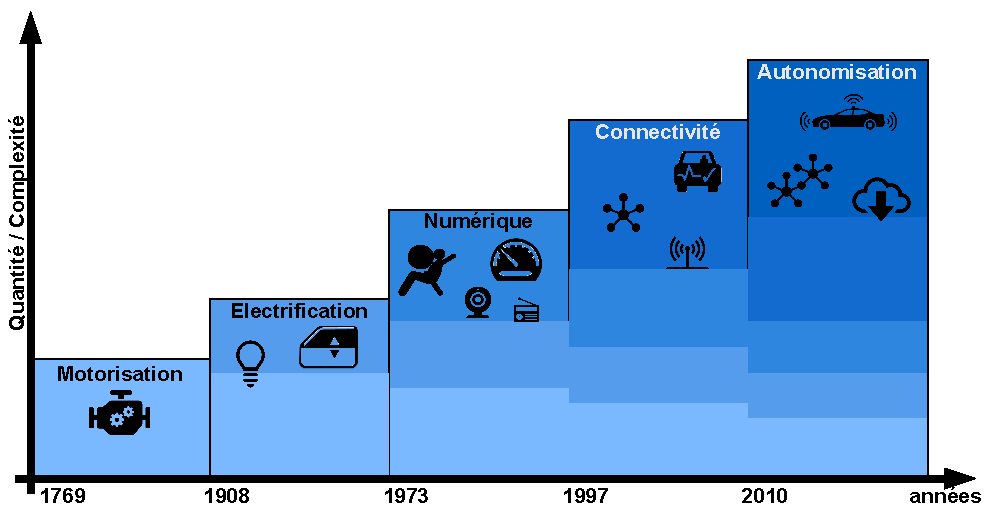
\includegraphics[width=0.9\linewidth]{schemas/Evo_Sys_Automobile}
			\caption[Évolutions des Systèmes Automobiles]{Principaux domaines d'évolution des systèmes automobiles au fil du temps}
			\label{fig:evo_sys_automobile}
		\end{figure}
	
		%%%%%%%%% Emergence des architectures EE actuelles GENERALISATION 
		De façon plus générale, le contexte industriel actuel fait émerger de nouvelles technologies basées sur des logiciels de plus en plus complexes et performants. Cela est rendu possible via l'émergence d'architectures matérielles toujours plus puissantes et performantes. Ces améliorations permettent le développement et la mise en application de nouvelles technologies comme les réseaux de communication sans fil haute performance ou encore l'usage d'intelligences artificielles. On retrouve ainsi un nombre grandissant de fonctionnalités directement embarquées dans l'automobile, l'avion, le train pour répondre à la fois à de nouveaux besoins fonctionnels~: assistance à la conduite/pilotage, tableaux de bord, etc. et à des besoins de confort d'usage~: info-divertissement, connectivité, automatisations...
		
		
		D'un point de vue logiciel, les mises à jour de systèmes embarqués incluent à la fois de nouvelles fonctionnalités critiques pour le bon fonctionnement du système, mais aussi l'ajout de fonctions moins critiques. Ces mises à jour de services non essentiels amplifient  la multiplicité des niveaux de criticités du logiciel embarqué et donc la cohabitation entre sous-systèmes critiques et sous-systèmes non-critiques que l'on pourrait qualifier de "confort".
		
		D'un point de vue matériel, il y a de fortes convergences sur les architectures employées dans les différents domaines. Historiquement, on retrouvait en premier lieu des calculateurs monocœurs. Cependant, les diverses évolutions d'exigences ont fait apparaître des limites en capacité de calcul. La montée en fréquence de fonctionnement atteint un seuil maximum à cause de la chauffe et la consommation que cela implique. Tandis que l'augmentation du nombre de transistors qui composent les processeurs arrive aux abords des limites physiques~: la taille de gravure du silicium arrive au même ordre de grandeur que la taille des atomes de silicium dont elle est composé. De fait, jusqu'à récemment encore, la Loi de Moore~\cite{thompson_moores_2006} sur la puissance des processeurs s'est vérifiée. Des premiers microprocesseurs Intel en 1971, avec quelques milliers de transistors de \SI{10}{\micro\metre}, l'on est aujourd'hui à plus de 1 milliards de transistors de près de \SI{10}{\nano\metre}. Mais à l'aune d'une gravure proche des \SI{2}{\nano\metre}, on environne les dimensions de 10 à 15 atomes et les effets de la physique quantique entrent en jeu. Par conséquent, l'on se dirige vers les limites des technologies actuelles pour poursuivre ces améliorations de puissance. Pour ces raisons, le plus grand levier de progression disponible aujourd'hui repose sur la parallélisation des unités de calcul, et donc la notion de calculateur multicœur, qui est apparue dès les années 1950~\cite{smotherman_history_2005}. Les fondeurs s'orientent vers des processeurs où la montée en puissance est assurée par la multiplication des unités de calcul (dit "cœurs") parallèles dans le processeur. On passe ainsi de monocœurs toujours plus petits et compacts à des duals/quadri cœurs... et l'on va aujourd'hui jusqu'à des supercalculateurs à plus de 128 cœurs. Tous ces changements se visualisent parfaitement avec l'évolution des caractéristiques des processeurs au fil des années en~\autoref{fig:processorstrend}, tel qu'agrégé par K. Rupp \cite{rupp_42_2020}. Cette évolution est la bienvenue dans tous les secteurs concernés, allant du grand public dans les ordinateurs, téléphones et autres multimédias jusqu'aux applications industrielles en passant par les usages de serveurs réseaux et centres de calculs. %
			%	
		\begin{figure}[h!]
			\centering
			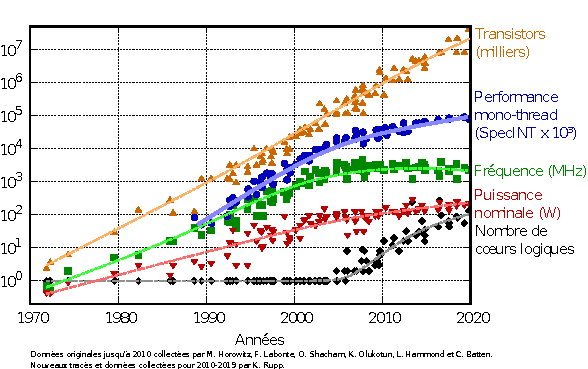
\includegraphics[width=0.8\linewidth]{graphiques/processors_trend}
			\caption[Évolution des processeurs]{42 Ans d'évolution des processeurs - Tendances}
			\label{fig:processorstrend}
		\end{figure}
		
		%%%%%%%% ARCHITECTURES MATERIELLES %%%%%%
		Il existe divers types d'architectures matérielles parmi les évolutions multicœurs que l'on retrouve aujourd'hui. On pourrait de façon simple différencier entre les multicœurs classiques, les manycœurs et à l'extrême ce que l'on connaît sous le nom de GPU, les processeurs graphiques.
		
		\paragraph{Multicœurs "classiques"} \label{Intro:multicoeurs}
		Les calculateurs multicœurs "classiques" disposent d'un certain nombre d'unités de calculs ("cœurs"), auxquelles sont adjointes diverses zones mémoires (cache, RAM, ROM). Le tout est piloté par des contrôleurs et bus de transfert de données pour interconnecter les cœurs, les cellules mémoires et les entrées/sorties. Dans les versions les plus récentes, des modules dédiés peuvent être ajoutés pour des fonctionnalités spécifiques comme le chiffrement.
			
		Il existe des variations d'architectures que l'on peut notamment distinguer entre d'une part les multicœurs basés sur le cache (comme celui susmentionné) qui sont prédominants et d'autre part les multicœurs basés sur \emph{scratchpad}, c'est-à-dire des mémoires locales dédiées à chaque cœur. On peut voir la différence fondamentale de structure entre ces deux variations sur la~\autoref{fig:ArchitecturesMulticoeur}.			
			
			\begin{figure}[h!]
				\centering
				\begin{subfigure}{.48\textwidth} 
					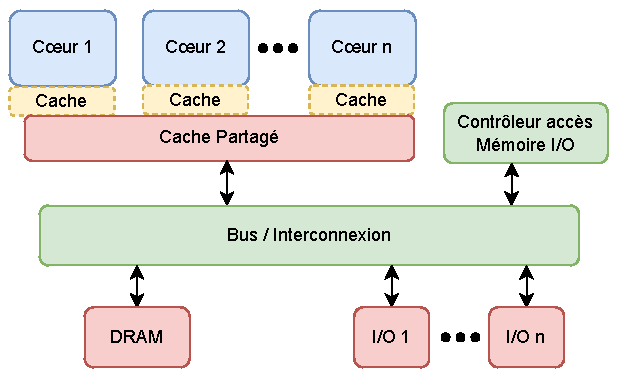
\includegraphics[width=\linewidth]{schemas/Multicore-CacheBased}
					\captionsetup{justification=centering}
					\caption[Diagramme Multicœur Cache]{Architecture calculateur multicœur basé sur le cache}
					\label{fig:multicoeurCache}
				\end{subfigure}
				\begin{subfigure}{.48\textwidth} 
					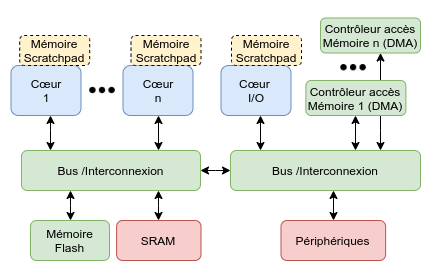
\includegraphics[width=\linewidth]{schemas/Multicore-ScratchpadBased}
					\captionsetup{justification=centering}
					\caption[Diagramme Multicœur Scratchpad]{Architecture calculateur multicœur basé sur scratchpad}
					\label{fig:multicœurScratchpad}
				\end{subfigure}
				\caption{Exemple multicœur et mémoires}
				\label{fig:ArchitecturesMulticoeur}
			\end{figure}
			
		Les architectures à Scratchpad mettent à disposition des mémoires à haut débit dédiées à chaque cœur. Toutes les ressources sont le plus possibles séparées entre les unités de calcul. Les modèles d'exécution de tâche sont en général très cadrés avec trois phases d'exécution (Chargement mémoire, exécution et déchargement) pour maîtriser le modèle d'exécution du logiciel. Les architectures Scratchpad sont alors des solutions en elles-mêmes aux problèmes d'exécution parallèle de code sur les calculateurs multicœurs pour éviter les problèmes d'interférences. Ce type de solutions par design limite en revanche les possibilités d'implémentation de logiciel de part cette spécificité de l'architecture matérielle.
			
		À l'inverse, les architectures basées sur le cache se veulent polyvalentes et comptent sur des mécanismes de contrôle logiciel pour optimiser l'utilisation des ressources.
		La mémoire est partagée à différents degrés entre les cœurs. De façon à décongestionner les accès mémoire et accélérer ces dernières, une hiérarchie mémoire est mise en place, associant des espaces mémoire progressivement plus petits et rapides en fonction de leur proximité au processeur. Il s'agit ici de trouver un équilibre entre coût de la mémoire et vitesse d'accès aux données. En effet,  cette dernière dispose de trois caractéristiques antagonistes~:
			\begin{itemize}
				\item la \textbf{latence} - temps d'accès aux données, 
				\item la \textbf{bande passante} - débit de données accessible,
				\item la \textbf{taille} mémoire - espace mémoire disponible (pour un coût donné).
			\end{itemize}
		Un espace mémoire pourra être soit de petite taille, mais rapide au niveau de son temps d'accès, soit de grande taille et plus lent comme schématisé dans la~\autoref{fig:hierarchiememoire}.  On a par conséquent au plus proche des cœurs les registres, de taille très limitée (octets) mais au temps d'accès très rapide~: ils sont la base pour toutes les opérations effectuées par le processeur. À l'opposé, la mémoire principale, de très grande taille (Go/To) pour laquelle tous les cœurs doivent passer par un bus commun pour y accéder. C'est donc la mémoire la plus lente d'accès, mais aussi la moins coûteuse. Plusieurs intermédiaires ont été mis en place entre ces deux types de mémoire. Il s'agit typiquement de niveaux de cache qui peuvent être non partagés, c'est-à-dire propres à chaque cœur ou bien commun à tous. Le dernier niveau de cache, partagé, est classiquement appelé LLC (\emph{Last Level Cache}) et donne la limite entre les espaces mémoire limités en cache avec des accès rapides d'une part et la mémoire principale qui va provoquer de grands ralentissements d'autre part. 			
		On retrouve ainsi avec l'exemple de la~\autoref{fig:multicoeurintel} un cas de calculateur multicœur basé sur le cache, avec 8 cœurs, des niveaux de cache mémoire séparés (L1 et L2) et partagé (L3) ainsi que le bus d'accès à la mémoire principale. 
		
		\begin{figure}[h!]
			\centering
			\begin{subfigure}{.42\textwidth} \centering
				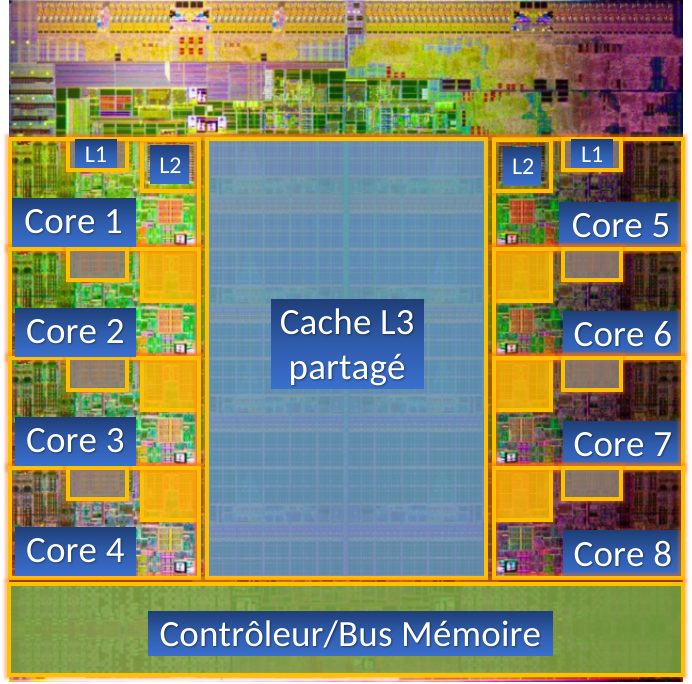
\includegraphics[width=0.9\linewidth]{schemas/multicoeurIntel}
				\caption{Exemple d'architecture multicœur}
				\label{fig:multicoeurintel}
			\end{subfigure}			
			\begin{subfigure}{.45\textwidth} \centering
				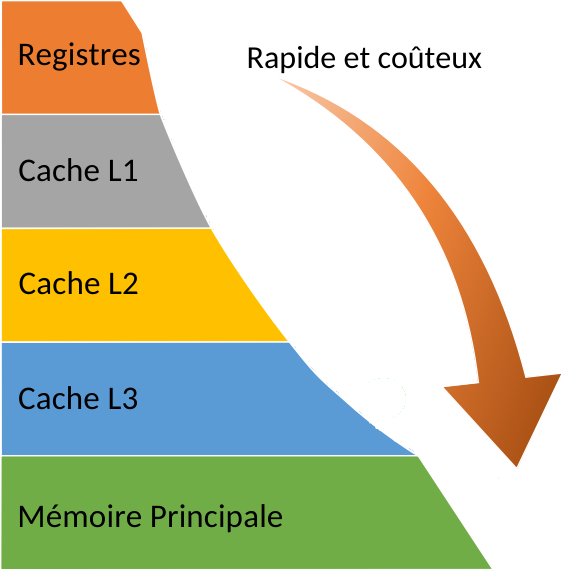
\includegraphics[width=0.85\linewidth]{schemas/hierarchieMemoire}
				\caption[Hiérarchie mémoire]{Schématisation de la hiérarchie \\mémoire selon leur coût et performance}
				\label{fig:hierarchiememoire}
			\end{subfigure}
			\caption{Exemple de multicœur Intel 17-5960X et hiérarchie mémoire}
			\label{fig:multicoeurs}
		\end{figure}
			
			%%%%% A DEPLACER DANS STRATEGIES EXISTANTES %%%%
		La gestion du contenu de ces caches (en lecture et écriture) est géré par une politique d'accès mémoire. Cette politique est essentielle à un usage efficace des caches du fait de leur espace limité qui demande à faire des choix sur son usage. Cela est peu documenté par les constructeurs, et chacun aura son propre algorithme.
		La méthode de base la plus répandue étant empirique, par principe de localité temporelle~\cite{durrieu_predictable_2014} et spatiale~\cite{wilkes_slave_1965}. On considère que plus une donnée a été récemment accédée, plus elle a de chance d'être à nouveau utilisée. De même si une donnée est sollicitée, alors les données proches spatialement ont aussi plus de chance d'être utilisées. 
		Nous n'iront pas plus dans les détails sur les politiques de gestion d'accès à la mémoire. Il faut garder à l'esprit qu'elle est plutôt subie par les industriels qui intègrent le matériel dans leurs systèmes. Pour un processeur donné on aura certaines performances de calcul et accès mémoire, et il faudra mettre en comparaison les performances "par défaut" d'un logiciel sur une architecture matérielle donnée face au même logiciel avec l'ajout de la surcouche de contrôle d'exécution apportées par l'intégrateur pour limiter les interférences.


		\paragraph{Calculateurs manycœurs}	Les calculateurs manycœurs sont des microprocesseurs incluant un grand nombre de cœurs dans l'objectif primaire d'une plus grande capacité d'exécution de code parallèle. Pour ce faire, les cœurs peuvent être spécialisés avec la réduction des instructions réalisables et optimisations à des tâches spécifiques. C'est la différence principale avec les multicœurs qui possèdent en en général des cœurs identiques (processeur homogène) avec de bonnes performances à la fois en série et en parallèle. 
		Les architectures manycœurs grâce à leurs spécificités demandent  des méthodes de programmation appropriées pour pouvoir être pleinement exploités dans le cadre d'une application. Cela augmente donc le niveau de complexité de développement, mais au bénéfice d'une forte amélioration des performances.
		
		Les GPUs (\emph{Graphic Processing Unit}) sont un cas particulier de manycœurs à présent très répandu pour des usages variés~\cite{owens_gpu_2008}. Cette forte expansion des GPU est due non seulement aux capacités de rendu graphique, mais surtout à leurs capacités de programmation parallèle poussée au maximum. Un grand nombre de domaines, notamment dans la recherche, y voient donc un microprocesseur d'usage général à hautes capacités de calcul parallèle.
		Les GPU sont efficaces du fait qu'ils permettent de réaliser le même calcul sur un très grand nombre de données différentes (typiquement calculs matriciels) pour obtenir tout autant de résultats en sortie. Il s'agit d'un modèle dit \emph{SIMD - Single-Instruction, Multiple-Data}. Là où les multicœurs conventionnels se focalisent sur des cœurs versatiles qui s'adaptent pour pouvoir gérer tous les cas d'applications, les GPU se focalisent sur la réalisation de tâches identiques en parallèles, ils restent donc spécialisés pour des types de tâches spécifiques, en complément de processeurs plus polyvalents.
		
		Dans le cadre de ces recherches, nous nous focaliseront sur le dénominateur commun le plus utilisé dans les architectures électriques et électroniques, qui est donc le processeur multicœur basé sur le cache.
		
\section{Risques et Problématique}
%%% Transition vers menaces
	Dans le cadre du contexte automobile, on se dirige \cmnt{de cette façon} vers un nouveau paradigme, où la voiture n'est plus un système mécanique sur lequel on adjoint du logiciel, mais à l'inverse un superordinateur multifonctionnel auquel on implante des roues et un moteur. 
	Les systèmes automobiles sont ainsi devenus des systèmes cyberphysiques qui entrent en interaction à la fois avec les utilisateurs et l'environnement. On distingue deux grands domaines de logiciels embarqués dans le véhicule. Tout d'abord l'info-divertissement, qui réunit les systèmes multimédias et autres affichages non nécessaires à l'usage primaire du véhicule. Et deuxièmement les calculateurs enfouis qui réalisent des fonctions essentielles qui ne sont pas nécessairement visibles de l'utilisateur, telles que le contrôle moteur. Pour soutenir ces besoins émergents, il est nécessaire de se baser sur des architectures matérielles plus puissantes comme les multicœurs. Cependant, cette disruption apporte de nouveaux enjeux, notamment de sécurité, vie privée, mais aussi sur la prédictibilité et la sûreté de fonctionnement du système à cause de sa complexification. Cela fait donc évoluer les systèmes embarqués dans un environnement profondément à risques, mais qui en plus s'accompagne de contraintes fortes. Nous nous devons donc d'introduire ici les notions de Sûreté de fonctionnement nécessaire à l'analyse.


	\subsection{Sûreté de Fonctionnement Informatique}~\label{sec:SureteDeFonctionnement}
		La sûreté de fonctionnement (SdF) d’un système informatique est "\textit{la propriété qui permet à ses utilisateurs de placer une confiance justifiée dans le service qu’il leur délivre, le service étant le comportement du système perçu par un utilisateur, cet utilisateur étant un système (informatique, humain, environnemental) qui interagit avec le premier.}"~\cite{laprie_guide_1996}. C’est donc la capacité d’un système informatique de répondre de manière correcte, conformément aux spécifications fonctionnelles, à une requête d’un autre système.  
		La sûreté de fonctionnement est définie en fonction de trois notions principales~: \linebullets{les \textit{attributs} qui définissent les propriétés assurées, les \textit{entraves} qui caractérisent les circonstances indésirables mais prévues, et les \textit{moyens} qui précisent les techniques permettant au système de fournir son service.} 
		Selon les services souhaités par l’utilisateur, ce dernier peut vouloir accentuer certaines propriétés pour assurer le bon fonctionnement du système. Ainsi la sûreté de fonctionnement englobe les attributs suivants~:  
		\begin{itemize}
			\item 	La \textbf{disponibilité} - la capacité d’être prêt à délivrer le service correct~; 
			\item 	La \textbf{fiabilité} - l’assurance de continuité d’un service correct~; 
			\item 	La \textbf{sécurité-innocuité} - l’assurance de non-propagation de conséquences catastrophiques à l’utilisateur ou l’environnement~; 
			\item 	L’\textbf{intégrité} - l’assurance de non-altération du système~; 
			\item 	La \textbf{maintenabilité} - l’aptitude à la réparation et à l’évolution du système. 
		\end{itemize} 
		Ces attributs permettent d’une part d’exprimer les propriétés devant être respectées par le système, et d’autre part d’évaluer la qualité du service délivré vis-à-vis de ces propriétés. Les aspects de sécurité, au sens de la confidentialité et des attaques face à des actions malveillantes indésirables ainsi que la confidentialité, c'est-à-dire, la non-divulgation d'information non autorisée, ne seront pas abordés dans cette thèse.

		\begin{figure}[h!]
			\centering
			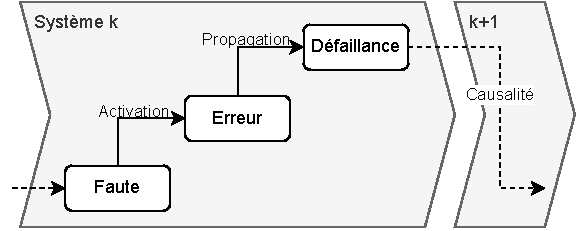
\includegraphics[width=0.7\linewidth]{schemas/SureteDeFonctionnement_Entraves}
			\caption{Sûreté de fonctionnement - chaîne de causalité}
			\label{fig:suretedefonctionnemententraves}
		\end{figure}
		
		Les entraves à la sûreté de fonctionnement sont les défaillances, les erreurs et les fautes. Une défaillance est une transition d’un service correct vers un service incorrect. Un service est considéré incorrect s’il n’est pas conforme à la spécification ou si la spécification ne décrit pas avec précision la fonction du système. Étant donné qu’un service consiste en une séquence d’états externes du système (observés par l’utilisateur), la survenue d’une défaillance signifie qu’au moins un des états externes s’écarte de l’état correct du service. La déviation est liée à une erreur, qui représente la partie de l’état interne du système pouvant entraîner une défaillance, dans le cas où elle atteint l’interface du service du système. La cause déterminée ou présumée d’une erreur est appelée une faute. La~\autoref{fig:suretedefonctionnemententraves} représente ce lien de cause à effet. Le fait de prévenir la causalité entre fautes est défaillances pour le bon fonctionnement se désigne par la méthode de silence sur défaillance. C'est-à-dire qu'une faute ou une erreur n'aura pas plus de conséquences et ne provoquera pas outre de défaillance, ou inversement.
	
		
		Pour minimiser l’impact de ces entraves, la sûreté de fonctionnement dispose de méthodes et techniques qui permettent de conforter les utilisateurs quant au bon accomplissement des fonctions du système. Le développement d’un système sûr de fonctionnement passe donc par l’utilisation combinée de ces méthodes, appelés moyens, pouvant être classées en quatre types~:
		\begin{itemize}
			\item \textbf{Prévision} des fautes~: estimation de la présence, de la création et des conséquences des fautes (p. ex. Analyse FMEA)~;
			\item \textbf{Prévention} des fautes~: méthodes visant à réduire les occurrences ou l’introduction de fautes (p. ex. outil de génie logiciel, processus de développement strict)~;
			\item \textbf{Élimination} des fautes~: réduction du nombre et de la sévérité des fautes (p. ex. test, injection de fautes)~;
			\item \textbf{Tolérance} aux fautes~: capacité de fournir un service, optimal ou dégradé, en présence de fautes (p. ex. techniques de redondance).
		\end{itemize}
	
		La prévention et la tolérance aux fautes visent à fournir la capacité de délivrer un service correct, tandis que l’élimination et la prévision des fautes visent à susciter la confiance en cette capacité en justifiant que les spécifications fonctionnelles de sûreté de fonctionnement et de sécurité sont adéquates et que le système est conforme. Toutes ces techniques sont dédiées à garantir des propriétés de sûreté de fonctionnement issues de spécification non fonctionnelles. % et non pas à délivrer un service applicatif.
		
		%%% PHRASE TRANSITION POURQUOI ON S'INTERESSE TaF
		\paragraph{Tolérance aux Fautes}
		Les fautes auxquelles un système doit faire face sont nombreuses et peuvent ne pas avoir d’impact sur celui-ci tant qu’un ou plusieurs évènements ne se sont pas produits. On les appelle alors des fautes dormantes. Une fois activées, ces fautes peuvent avoir un impact catastrophique sur le système. D’origines diverses et variées, certaines fautes sont dues à l’environnement, au matériel, ou encore à l’être humain.
		
		Chaque faute peut provoquer une ou des erreurs différentes pouvant entraîner la défaillance du système. Malgré l’application des techniques de prévention et d’élimination des fautes, certaines subsistent et sont à même d’être activées.
		
		Un système tolérant aux fautes doit pouvoir assurer à l’utilisateur un service correct en dépit des fautes pouvant altérer ses composants, durant sa conception ou son interaction avec d’autres systèmes~\cite{avizienis_basic_2004}. La Tolérance aux fautes est mise en œuvre grâce aux moyens de \textbf{détection} d’erreurs, c.-à-d., l’identification des déviations du service correct, et de \textbf{recouvrement}, c.-à-d., les techniques permettant en cas d’erreur détectée de passer d’un état de système fautif à un état assurant un service nominal ou dégradé.
		
		La détection d’erreur peut être soit concurrente et se déroulant pendant l’exécution du système soit anticipée en vérifiant les paramètres du système lors de la suspension de son exécution. Une fois cette erreur détectée, les techniques de recouvrement peuvent être employées, d’une part pour assurer le service désiré et éviter la propagation de l’erreur (traitement des erreurs) et d’autre part pour isoler le composant fautif, diagnostiquer l’erreur, trouver et déterminer la faute originelle pour assurer une opération de maintenance (traitement des fautes).
		
		Les techniques de détection et de recouvrement sont nombreuses et sont regroupés dans des mécanismes de tolérance aux fautes associés à un ou plusieurs types de fautes. Il n’y a à l’heure actuelle aucun mécanisme générique pouvant pallier n’importe quel type de fautes ou d’erreurs. Que cela soit de la redondance matérielle, logicielle, temporelle, de la diversité dans l’implémentation ou l’architecture, les techniques sont nombreuses et souvent propres à chaque domaine et au budget alloué à la tolérance aux fautes.
		
		Dans le cadre de ces travaux de recherche, nous nous intéresseront particulièrement à la tolérance aux fautes qui a trait donc à la bonne exécution de tâches hébergées au sein d'un même calculateur. Dans le contexte industriel susmentionné, un même calculateur exécute des tâches pour des fonctionnalités variées et par conséquent avec des niveaux de criticité variés. Cela engendre notamment des contraintes sur les temps d'exécution des logiciels les plus critiques. C'est ce qu'on qualifie de systèmes temps réel. Nous sommes en résumé dans un contexte à criticité mixte, où du logiciel de système temps-réel va coexister avec du logiciel avec des contraintes temporelles moins strictes, voire aucune contrainte. L'implémentation de mécanismes de sûreté de fonctionnement dans ce contexte-là relève alors de la gestion de fautes temporelles dans un système à criticité mixte. 
		
\subsection{Systèmes temps-réel et Ressources partagées}
	\paragraph{Système temps-réel}~\label{sec:SystemesTempsReels}
	Les systèmes embarqués sont conçus sur la base d'un modèle de capteurs et actionneurs. Les capteurs représentent l'ensemble des éléments qui permettent d'obtenir les données d'entrée au système de façon à ce qu'il puisse réaliser sa fonction. Il s'agit notamment des informations de l'environnement du véhicule, mais aussi des données internes avec tout l'état de fonctionnement actuel ainsi que les interactions avec l'utilisateur. Ces informations sont alors gérées par les calculateurs de décision via des algorithmes plus ou moins complexes. Le logiciel permet donc à partir de ces données d'entrée de calculer les commandes qui sont dirigées vers les actionneurs. Les actionneurs sont alors en bout de chaîne afin d'accomplir la commande. Dans le cas où les données d'entrée fournies par les capteurs sont liées aux données de sortie, on parle alors d'une \emph{boucle} de contrôle. Typiquement avec le chauffage d'un logement qui utilise un capteur de température pour une consigne de température donnée.
		
	Prenons un exemple hypothétique de contrôle de l'injection moteur pour une voiture. En entrée, le calculateur de contrôle moteur récupère entre autre les informations du capteur de vitesse de rotation du moteur, de la quantité d'essence en réservoir et l'accélération demandée par le conducteur. Il peut alors calculer l'instant et la quantité de carburant qu'il sera nécessaire d'injecter dans le moteur. Cette commande est alors transmise à l'actionneur, l'injecteur, pour être réalisée. Et ce bloc de contrôle-commande doit se répéter périodiquement pour suivre la consigne tout le long de l'utilisation du véhicule.
		
	Tous ces éléments de contrôle-commande ont en commun d'avoir des contraintes temporelles. Le temps de réaction --qui définit la durée entre la récupération des données des capteurs jusqu'à la réalisation de la commande par les actionneurs--  peut alors être une donnée critique pour certaines applications comme l'exemple donné ci-dessus (\textit{inutile de dire qu'un contrôle d'injection moteur qui prend trop de temps à déterminer combien de carburant injecter aura des conséquences bien évidemment indésirables...}). Ainsi, ce genre d'applications nécessite à la fois de retourner des résultats corrects, mais aussi de les délivrer dans les temps. 
		
		\begin{figure}[h!]
			\centering
			\begin{subfigure}{.3\textwidth} \centering
				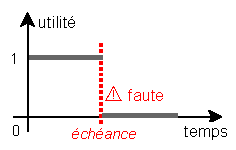
\includegraphics[width=\linewidth]{schemas/SdF_TempsReelDUR}
				\caption[]{Temps-réel Strict}
				\label{fig:tempReelDur}
			\end{subfigure}
			\begin{subfigure}{.3\textwidth} \centering
				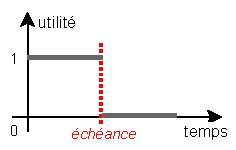
\includegraphics[width=\linewidth]{schemas/SdF_TempsReelFERME}
				\caption[]{Temps-réel Ferme}
				\label{fig:tempReelFerme}
			\end{subfigure}
			\begin{subfigure}{.3\textwidth} \centering
				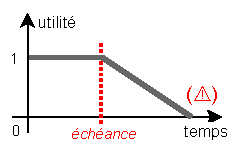
\includegraphics[width=\linewidth]{schemas/SdF_TempsReelMOU}
				\caption[]{Temps-réel Souple}
				\label{fig:tempReelMou}
			\end{subfigure}
			\caption{Modèles d'utilité des résultats d'une tâche temps-réel}
			\label{fig:ModelesTempsReel}
		\end{figure}
		
		Plus généralement, les applications embarquées se caractérisent par un ensemble de tâches logicielles qui interagissent entre-elles. Elles sont soit périodiques (c.-à-d. exécutés à intervalle réguliers) soit apériodique (sur réception d'un événement). Chaque tâche possède ses spécifications propres en termes de données d'entrée, de sortie ainsi que ses paramètres d'exécution (selon les cas : période, niveau de priorité, allocation physique) dont une échéance d'exécution. Les systèmes temps-réel peuvent se catégoriser en 3 catégories qui sont schématisées en~\autoref{fig:ModelesTempsReel}. On retrouve d'une part les systèmes \textbf{temps-réel strict} ("\textit{hard real-time}") où le respect de l'échéance est strict en~\autoref{fig:tempReelDur}. Il est alors considéré qu'une tâche dont le temps de réponse dépasserait l'échéance serait une faute temporelle indésirable et les données renvoyées par la tâche n'ont plus de valeur. Le même modèle mais sans conséquences après dépassement de l'échéance est nommé \textbf{temps-réel ferme} ("\textit{firm real-time}") illustré en~\autoref{fig:tempReelFerme}. À l'inverse, les systèmes \textbf{non-temps-réel} n'imposent pas de contraintes d'échéance sur l'exécution des tâches. Il s'agit donc de faire au mieux, mais tout dépassement des temps d'exécution nominaux n'a pas de répercussions. C'est ce que l'on côtoie couramment via nos appareils de tous les jours comme le smartphone ou l'ordinateur. Enfin, les systèmes \textbf{temps-réel souple} ("\textit{soft real-time}") sont un entre-deux où l'échéance représente un seuil limite au-delà duquel la valeur de retour de la tâche garde une utilité pour le système mais qui décroît avec le temps, jusqu'à ne plus être pertinente comme représenté en~\autoref{fig:tempReelMou}. On dit alors que la donnée est "périmée". Ce dépassement peut alors provoquer ou non une faute.
		
		Les analyses d'exécution temporelles des tâches constituent alors un aspect essentiel du développement de logiciel critique afin de garantir le respect des échéances. Cela peut se faire soit de façon expérimentale ou théorique. L'objectif étant de vérifier l'ordonnancement, c'est-à-dire la bonne gestion de l'exécution du logiciel sur le processeur suivant les contraintes imposées (échéances, dates d'activation, périodes...). Un système est dit prédictible si l'on est capable de prouver de façon théorique que les contraintes temporelles seront respectées. Cela se fait par le biais d'analyses d'ordonnançabilité. Un technique classique de ce type d'analyse consiste à évaluer les pires temps d'exécution ("\textit{Worst-Case Execution Time -- WCET}"). Le WCET indique la durée maximum au-delà de laquelle on sait qu'en toutes conditions, la tâche correspondante aura terminé son exécution. Il est possible de comparer les WCET des tâches avec leurs échéances. Pour du temps réel strict, les valeurs de WCET se devront d'être strictement inférieures aux échéances, là où pour du temps réel ferme ou souple on pourra se contenter d'estimation ou de résultats statistiques.
				
		Au sein d'un même processeur, toutes les tâches n'auront potentiellement pas les mêmes types de contraintes d'exécution. Mais en plus de cela, les architectures matérielles multicœurs complexifient d'autant plus l'analyse. 
		
		
	\paragraph{Ressources Partagées}
	
	Comme nous l'avons vu précédemment sur l'architecture multicœur, il existe un bon nombre de ressources qui sont partagées entre les différents logiciels qui sont exécutés. Ces partages de ressources peuvent influencer directement sur l'exécution des tâches et donc sur leur capacité à respecter les échéances. En effet, si plusieurs tâches ont des besoins concurrents d'accès à une même ressource alors nécessairement l'une va passer avant l'autre. Cette dernière sera \textit{de facto} retardée dans son exécution. Il existe ainsi de nombreuses sources de retards potentiels d'exécution~\cite{kotaba_multicore_2013}~: 
	\begin{itemize}
		\item Mémoire --
		\begin{itemize}[label=$ \circ $] %\bigstar \blacklozenge \blacksquare \blacktriangle \blacktriangledown \lozenge \Diamond  \bullet
			\item 	erreurs en lecture~: si une donnée n'est plus présente en cache du fait qu'elle a été remplacée par les données d'une autre application. Cela demande alors à remonter sur les niveaux de mémoire supérieurs, ce qui engendre des temps d'accès supplémentaires importants ;
			\item 	accès concurrents : l'accès concurrent à un niveau de mémoire partagée se fait par le bien d'un contrôleur d'accès mémoire, qui va devoir arbitrer sur l'ordre et le temps alloué à chaque tâche.
			\item 	Cohérence mémoire : selon les technologies de gestion de cache utilisées, il faut gérer la cohérence mémoire. Si une donnée est utilisée dans plusieurs mémoires non partagées, alors il faut s'assurer que la donnée en question reste cohérente entre toutes les tâches qui s'en servent. Cela implique en général une synchronisation sur les niveaux de mémoire supérieure quand elle est modifiée de façon locale, et inversement une propagation des modifications vers les tâches qui manipulent la donnée.
		\end{itemize}
		\item Périphérique et I/O en général --
			chaque périphérique dispose de son propre contrôleur d'accès. On a donc les mêmes enjeux qu'avec les accès concurrents à la mémoire dans le cas où plusieurs tâchent utilisent la même entrée/sortie. Le cas principal ici pour une architecture embarquée est sur l'utilisation d'un bus de communication externe qui sert à interconnecter les calculateurs. L'envoi et la lecture de message sur de tels bus de communication peuvent alors engendrer un grand nombre d'usages concurrents. 
		\item Bus d'interconnexion -- 
			Le fonctionnement même des processeurs implique l'utilisation de bus internes afin de gérer la transmission et le stockage de données. Tout usage de ces bus d'interconnexion peuvent alors impliquer des usages concurrents qui impactent l'accès aux données des tâches.
		\item Puissance de calcul -- 
			Enfin, mais pas des moindres, il n'y aura probablement jamais autant de cœurs que de tâches sur un processeur multicœur. Il est de ce fait évident que les tâches devront se partager tout ou partie des cœurs selon leur allocation physique. C'est là que va entrer en jeu la stratégie d'ordonnancement des tâches. La politique d'ordonnancement joue un rôle essentiel pour permettre le respect des contraintes temporelles et optimiser l'usage de la puissance de calcul pour limiter au maximum les temps d'attente en file d'exécution des tâches. 
	\end{itemize}

	Par conséquent, les contraintes majeures de prédictibilité d'exécution au sein de calculateurs multicœurs est mise à mal. La multiplication des points de contention rendent les analyses de pire temps d'exécution plus complexe. C'est d'autant plus le cas avec la prise en compte de dépendances logicielles (synchronisations) et matérielles (gestion des accès concurrents à des ressources partagées). Cela requiert un bon nombre de compromis sur l'exploitation des ressources matérielles pour compenser cette complexité et conserver les objectifs de prédictibilité d'exécution habituellement recherchés.

\subsection{Problématique et Objectifs}
		Dans le contexte industriel qui concerne notre étude, les évolutions des systèmes cyberphysiques présentés précédemment impliquent que des tâches de différents modèles d'exécution doivent être intégrées au sein d'un même multicœur. On parle alors de système à criticité mixte. Cette coexistence de fonctionnalités va augmenter la complexité d'étude de sûreté de fonctionnement afin de garantir l'ordonnançabilité des tâches et le respect des contraintes temporelles. Et comme nous venons de le voir, les nouveaux calculateurs multicœurs ajoutent en niveau de complexité avec l'augmentation de risque d'interférence entre logiciels concurrents. Il devient par conséquent de plus en plus complexe de mener des études théoriques pour estimer les pires temps d'exécution et donc l'ordonnançabilité des tâches. La conséquence directe à cela est un manque de garanties claires sur le bon respect des échéances temporelles pour les tâches les plus critiques pour lesquelles on ne peut se permettre de telles fautes.
		
		On verra qu'il existe de nombreuses méthodes qui permettent de réduire les interférences et donc fiabiliser les études d'ordonnançabilité. Cependant, cela se fait en général au prix d'un compromis sur les performances de calcul.
		Hors, c'est pour cette même puissance de calcul que la transition vers des calculateurs multicœurs s'est faite. Il semble alors essentiel de vouloir l'exploiter au maximum. On a deux objectifs qui s'opposent, mais qui sont tout autant essentiels. D'une part l'exploitation au maximum des capacités de calcul pour héberger tout le logiciel nécessaire aux nouvelles fonctionnalités des systèmes embarqués. D'autre part continuer à donner des garanties fortes de respect des contraintes temps réel pour les tâches critiques. 
		
		Cela nous mène donc à la problématique centrale de cette thèse, qui est d'identifier les leviers et mécanismes qui peuvent permettre d'atteindre au mieux les deux objectifs susmentionnés d'optimisation de l'usage du processeur avec les garanties temporelles liées aux systèmes critiques. 
		Nous tenterons dans la suite de proposer une réponse à cette problématique par le biais d'une nouvelle approche qui mène à l'usage d'un mécanisme de surveillance et de contrôle de l'exécution des tâches pour éviter toute faute temporelle en cas d'occurrence d'interférences tout en permettant par ailleurs de libérer toute la puissance de calcul disponible dans l'exécution des tâches.
	

\section{Contraintes et Hypothèses}
		
	\subsection{Contexte industriel Automobile}
		Cette problématique s'inscrit dans un contexte industriel aux contraintes spécifiques. Il est donc important d'avoir ces éléments en ligne de compte pour proposer une analyse et des contributions pertinentes. Historiquement dans le domaine automobile, les calculateurs embarqués étaient conçus de manière \emph{ad hoc}. Le logiciel et le matériel étaient intimement liés. Cela conduit à un nombre de calculateurs très important, chaque calculateur apportant une fonctionnalité qui lui est propre. Les architectures se composent alors d'un grand nombre d'unités de calcul interconnectées. 

		Ce type d'architecture distribuée présente des inconvénients évidents en terme d'évolutivité du système et de coût de développement. À chaque changement de support physique le logiciel doit passer par un nouveau stade de développement plus ou moins conséquent. Inversement, une mise à jour du logiciel ou un ajout de fonctionnalité demande une prise en compte de l'intégration matérielle avec potentiellement des modifications matérielles pour suivre les évolutions. Chaque ajout de fonctionnalités va de cette façon ajouter de nouveaux calculateurs dédiés, complexifiant d'autant plus l'architecture.
		
		Toutes ces contraintes de développement s'inscrivent dans un contexte bien cadré par des normes et standards. L’architecture fédérée telle qu'elle arrive dans les architectures électriques et électroniques abolit la séparation physique qui préexistait entre les composants logiciels, par leur agrégation dans un nombre réduit de calculateurs plus puissants. Cela résulte en un accroissement de la complexité de l’intégration et de la mise en œuvre de la sûreté de fonctionnement. 
	
		\subsection{Standards industriels et Concept de Criticité}	
		Les processus de développement de systèmes embarqués sont régis par des standards qui donnent des garanties sur le bon fonctionnement et donc vis-à-vis du respect des contraintes non fonctionnelles. Ces standards recommandent des directives de développement qui suivent toutes la durée du processus, de la spécification jusqu'aux tests de validation et d'intégration. Une des normes "mères" de la sûreté de fonctionnement des architectures électriques et électroniques est IEC-61508~\cite{iec61508}. Il s'agit d'un standard européen générique qui touche donc à de nombreux domaines tels que le ferroviaire, l'automobile, l'aéronautique, etc. Il s'agit en particulier des systèmes où il existe des risques pour les personnes ou sur l'environnement en cas de défaillances. Ce standard définit des niveaux de criticité SIL (\textit{Safety Integrity Level}). Cela fourni des niveaux de fiabilité requis pour chaque niveau de criticité ainsi que les méthodes applicables pour atteindre cet objectif. Ce standard a été par la suite décliné suivant les domaines. Dans l'automobile est ainsi apparue en 2011 la première version d'ISO 26262, "Véhicules Routiers - Sécurité fonctionnelle~\cite{iso_tc22sc3wg16_iso_2011}. 

		
		La norme ISO 26262 est la norme de référence pour la sûreté de fonctionnement dans le domaine automobile. Elle recommande des méthodes et mécanismes, applicables durant toutes les phases de développement du véhicule, pour atteindre et justifier son niveau de sûreté de fonctionnement. La norme préconise d’effectuer une phase d’analyse des risques pour identifier les situations dangereuses et les classifier en 4 niveaux de criticités nommés ASIL (\textit{Automotive Safety Integrity Level}) allant du moins critique (ASIL A) au plus critique (ASIL D). Pour la détermination de ces niveaux, trois critères sont pris en compte: la sévérité, la probabilité d'accomplissement et la contrôlabilité.
		
		\begin{itemize}
			\item 		\textbf{La Sévérité}	\\
			Les conséquences en cas de défaillance peuvent être Légères et Modérées (\emph{S1}), Sévères et potentiellement mortelles -- mais survie probable -- (\emph{S2}), Potentiellement mortelles -survie incertaine- voire mortelles (\emph{S3}). 		
			\item 		\textbf{La Probabilité} 	\\
			Le risque d'occurence peut être Très Faible (\emph{E1}), Faible (\emph{E2}), de probabilité Moyenne (\emph{E3}) ou de Haute probabilité (\emph{E4}).
			\item 		\textbf{La Contrôlabilité}	\\
			Les capacités de l'utilisateur à gérer la défaillance. Une défaillance peut être facilement contrôlable (\emph{C1}), normalement contrôlable (\emph{C2}), difficilement, voire impossible à contrôler (\emph{C3}).
		\end{itemize}
		
		Bien entendu, l'interprétation de ces trois critères doit se faire au regard du système étudié, et non de façon absolue et déterministe. 
		Ces critères donnent lieu à une table de classification qui définit alors le niveau d'ASIL des composants tel que décrit dans le~\autoref{tab:ASILTable}. On remarquera le niveau "QM" pour \textit{Quality Management}, qui correspond aux composants qui n'impliquent pas de criticité particulière et peuvent alors être développés "au mieux" sans contrainte spécifique. Il est bien entendu moins critique qu'un ASIL A. Avec cette table on connaît alors le niveau de confiance que l'on va imposer à chaque composant pour qu'il puisse être utilisé de façon sûre de fonctionnement. Plus un composant sera critique, plus son niveau d'ASIL sera élevé en conséquence, et donc plus il faudra apporter d'efforts pour qu'il respecte les standards.
		
		On peut mentionner de la même manière d'autres standards équivalents dans l'avionique, DO-176 où les niveaux de criticité sont désigné en DAL ("\textit{Design Assurance Level}"), ou encore le ferroviaire avec CENELEC 5012x, mais aussi dans le nucléaire, le spatial, l'automatique, le médical... La plupart dérivés de IEC-61508.  Un certain nombre de ces standards ont été comparés dans les travaux de~\cite{baufreton_multi-domain_2010}. On y retrouve un point commun qui nous intéresse tout particulièrement ici qui est sur les contraintes temporelles.

		\newcommand{\red}{\ccolor{red}} \newcommand{\oran}{\ccolor{orange}} 
		\newcommand{\yel}{\ccolor{yellow}} \newcommand{\gr}{\ccolor{Green}}
		\begin{table}[h!]
			\centering
			\caption{Matrice de Définition des Niveaux d’ASIL - ISO 26262}
			\label{tab:ASILTable}
			\begin{tabular}{@{}ccccccccccccc@{}}
				\toprule
				&           & \mc{11}{c}{Contrôlabilité}  \\
				\cmidrule{3-13}
				&           & \mc{3}{c}{\cellcolor{Green}{C1}} & \phantom{} & \mc{3}{c}{\cellcolor{yellow}{C2}} & \phantom{} & \mc{3}{c}{\cellcolor{orange}{C3}}  \\
				\cmidrule{2-2}	\cmidrule{3-5}		\cmidrule{7-9}		\cmidrule{11-13}
				\mc{2}{r}{Sévérité}  & \gr{ S1 } & \yel{ S2 } & \oran{ S3 } &          & \gr{ S1 } & \yel{ S2 } & \oran{ S3 } &			  & \gr{ S1 } & \yel{ S2 } & \oran{ S3 } \\
				\midrule
				&  \gr{ E1 }  &    QM   &    QM     &    QM      &            &    QM    &     QM     &     QM      &			&    QM     &     QM     &   \gr{ A }	\\
				& \yel{ E2 }  &    QM   &    QM     &    QM      &            &    QM    &     QM		&  \gr{ A }   & 		&    QM     &  \gr{ A }  &  \yel{ B }	\\
				& \oran{ E3 } &    QM   &    QM     &  \gr{ A }  &            &    QM    &  \gr{ A }	&  \yel{ B }  &			& \gr{ A }  & \yel{ B }  & \oran{ C }	\\
				\mrQ{Probabilité} & \red{ E4 }  &    QM   & \gr{ A }  & \oran{ B } &            & \gr{ A } & \oran{ B }	
				& \oran{ C }  & 		& \yel{ B } & \oran{ C } &  \red{ D }	\\
				\bottomrule
			\end{tabular}
		\end{table}
		
		Que ce soit IEC-61508 ou plus spécifiquement ISO 26262, il est clairement stipulé que 
		"\textit{les contraintes temporelles des fonctions à durée critique doivent être gérées par les spécifications de sûreté de fonctionnement logicielle. Ici, à la fois les pires temps d'exécution au niveau du code et les temps de réponse au niveau système doivent être considérés.}". Et précisément, "\textit{l'absence de tout interférence se doit d'être assuré et, tout comme dans IEC-61508, le logiciel est sujet au plus haut niveau d'ASIL impliqué quand l'indépendance temporelle entre les fonctionnalités ne peut être assurée.}"~\cite{iso_26262-7_road_2018}. C'est au regard de ce type de contrainte industrielle qu'il est essentiel de proposer de nouvelles solutions avec l'arrivée de calculateurs multicœurs qui complexifient grandement les garanties de non-interférence.
	
	\subsection{Contraintes d'intégration}
			
	De façon plus générale, les enjeux industriels peuvent varier selon les domaines. Ceci étant dit on peut nommer des points principaux, qui sont ceux que l'on va tenter de prendre en considération dans cette étude. La première d'entre elle est l'imposition de capacités de déploiement rapides ("\textit{Time-to-market}" réduit). Les itérations entre générations demandent des coûts de développement les moins importants possibles. Cela permet des cycles courts et réactifs qui s'adaptent aux évolutions technologiques. Cette contrainte industrielle est structurante sur les choix de conception, ce qui nous ramène souvent au principe "\emph{KISS}" pour "\emph{Keep It Safe and Simple}" dans notre cas. C'est une philosophie que j'ai souhaité maintenir au long de cette thèse afin de tenter une approche un peu différente des principales recherches actuelles qui tentent souvent d'aller dans des niveaux de détails toujours plus précis et complexes pour répondre aux difficultés technologiques, au détriment d'une facilité d'implémentation qui permettrait une appropriation industrielle. Comme on le verra plus tard, il existe ainsi des solutions très sophistiquées qui donnent de bons résultats théoriques, mais qui ne se sont pas généralisés. Les questions de complexité d'implémentation et simplicité de maintenance dans un cas réel semblent donc relativement déterminantes pour mesurer la pertinence d'une nouvelle contribution à la sûreté des systèmes embarqués. 
	
	En ce sens, il existe globalement 3 types de sous-systèmes qui sont intégrés par les constructeurs. 
	D'abord les systèmes en \textit{black box} ou "boites noires" qui sont entièrement conçu par un équipementier tiers à partir de spécifications. Le contenu de ces "boites" est alors inconnu dans ses détails.
	Ensuite les systèmes en \textit{white box} où à l'inverse, la totalité de sa conception et de son modèle est connu. Cela permet des tests bien plus en profondeur et donc une plus grande confiance en son comportement. Pour être des "boites blanches" les composants sont en général soit directement faits par l'intégrateur final, soit fourni en open-source (plus rare, tristement).
	Enfin, il y a tout l'entre-deux de composants contenants à la fois des éléments en "boite noire" et en "boite blanche", que l'on appelle naturellement "boites grises".
	Il est très important de noter par ailleurs une catégorie transverse des systèmes \textit{Legacy}, qui sont des composants où les altérations et modifications sont impossibles pour diverses raisons. Soit parce qu'il s'agit d'une black box que l'on ne souhaite ou ne peut remplacer, soit pour des raisons de compatibilité restreinte où toute modification risquerait de compromettre la totalité du système intégré. 
	Ces différents types de sous-systèmes sont importants à présenter, car tout ce qui va toucher aux boites noires et aux composants \textit{legacy} ajoutent une contrainte forte sur le développement de solutions à la sûreté de fonctionnement. De fait, tout mécanisme de sûreté de fonctionnement impliquant la modification ou l'adaptation du code de fonctions intégrées au système risque d'être éliminé d'office !
	
		\begin{figure}[h!]
		\centering
		\begin{subfigure}{\textwidth} \centering
			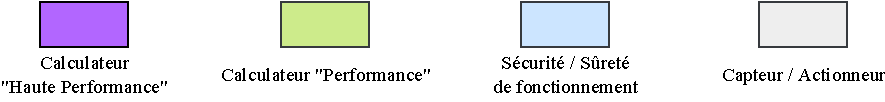
\includegraphics[width=\linewidth]{ArchitectureLegende}
			%\caption[something]{something}
			%\label{fig:something}
		\end{subfigure}
		\newline
		\begin{subfigure}{0.5\textwidth} \centering
			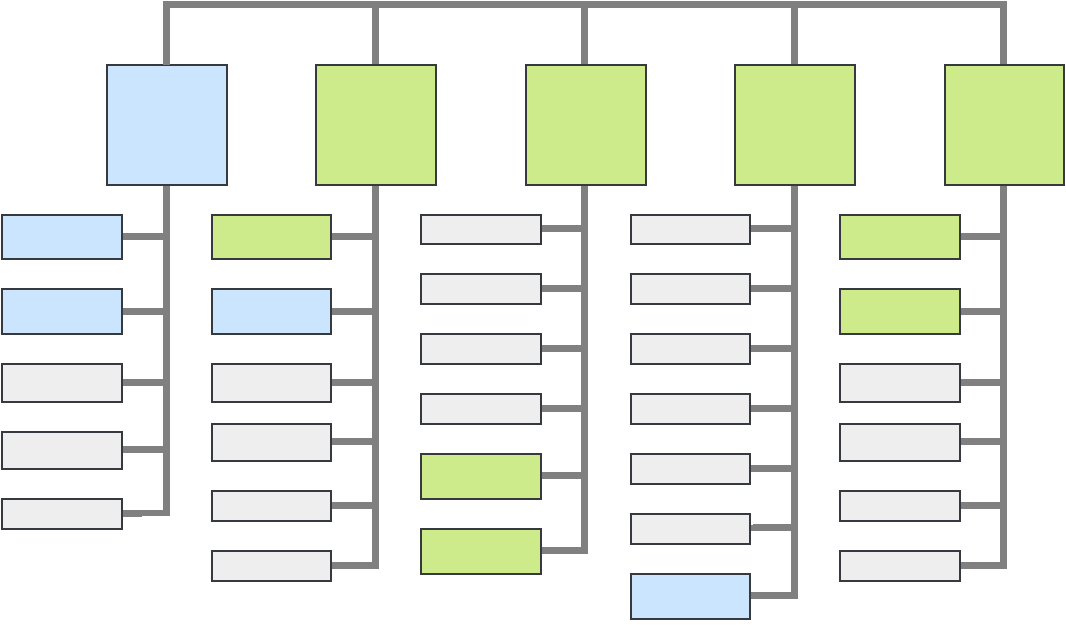
\includegraphics[width=\linewidth]{ArchitectureDistribuee}
			\caption{Architecture Distribuée}
			\label{fig:ArchiDistrib}
		\end{subfigure}
		\begin{subfigure}{0.45\textwidth} \centering
			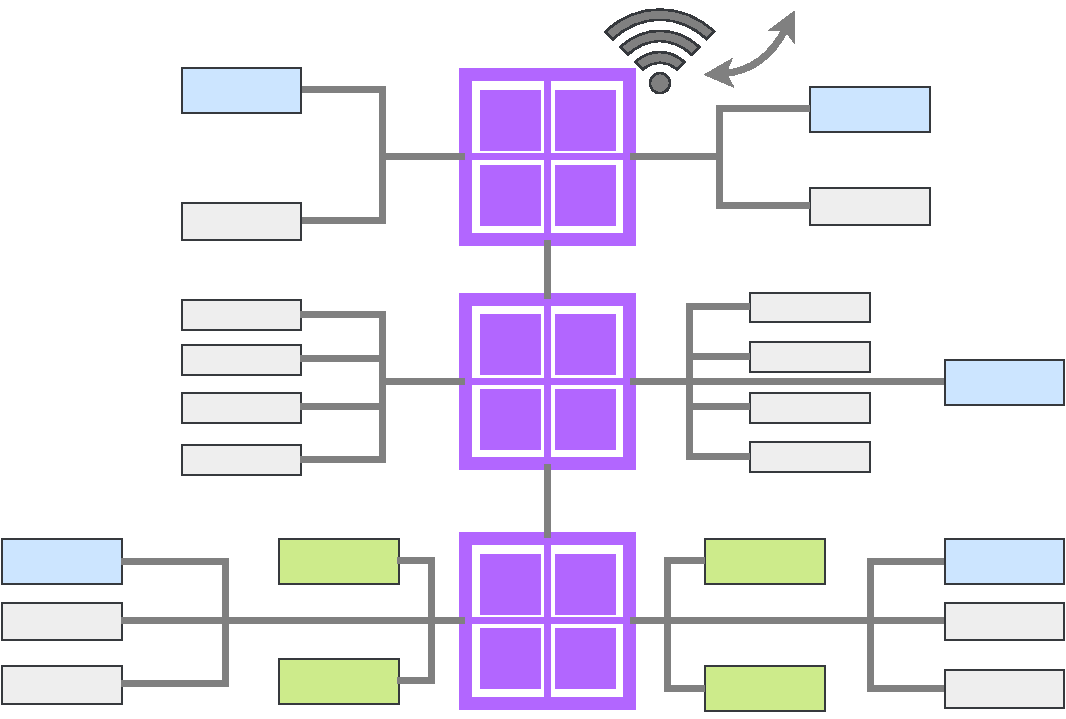
\includegraphics[width=\linewidth]{ArchitectureFederee}
			\caption{Architecture Fédérée}
			\label{fig:ArchiFederee}
		\end{subfigure}
		\caption{Architectures Electrique/Electronique (AUTOSAR)}
		\label{fig:ArchitecturesEE}
	\end{figure}

	On pourra pour finir, mentionner des enjeux plus divers tel que les contraintes d'encombrement. Les systèmes embarqués ont une forte tendance à la miniaturisation pour des raisons diverses selon les domaines. Cela permet une réduction de poids, essentiel pour tous les systèmes volants (avions, drones...) mais aussi d'encombrement pour des domaines comme l'automobile ou le ferroviaire qui doivent en toute circonstance rester dans des dimensions standards. Cette contrainte se fait beaucoup sentir avec l'arrivée des voitures autonomes par exemple, où les premiers prototypes --~bien que fonctionnels~-- se sont avérés trop chargés et encombrants avec le surplus d'équipement pour être transposables facilement en produits commercialisables tel-quel.
	
	Au regard de ces enjeux, l'évolution future naturelle est de réduire le nombre de calculateurs embarqués, en passant d'un grand nombre d'unités de calcul à une quantité limitée de "supercalculateurs", qui vont agréger différentes tâches. On passe de cette façon d'un système distribué à un système fédéré basé sur des calculateurs primaires accompagnés de processeurs satellites qui gèrent le strict nécessaire à hauteur des différents capteurs/actionneurs. Cette différence d'architecture est illustrée en~\autoref{fig:ArchitecturesEE} Cela permet de réduire les coûts et l'encombrement, qui va diminuer par la même occasion la quantité de câblages requis. Ce type d'architecture va faciliter l'évolutivité qui sera donc bien plus axée sur des mises à jour logicielles sans toucher au matériel. La connectivité permet de mettre en œuvre le concept du véhicule \textit{"as-a-service"}, qui va pouvoir évoluer et se mettre à jour régulièrement à distance (\textit{Over-the-Air Updates}). 
	
	
\section{Grandes approches du domaine}

	Nous verrons plus en détail dans le~\autoref{chap:2_StateofArt} les différentes solutions actuelles qu'il existe dans le domaine pour répondre à ces problématiques. Nous pouvons tout de même d'ores-et-déjà présenter fondamentalement sur quoi reposent les principes existants afin de mieux situer notre axe de recherche.
	
	La problématique principale à laquelle nous devons faire face réside dans la gestion des interférences matérielles de façon à éviter des fautes temporelles ou tout du moins à couper la chaîne de causalité de façon à ce qu'il y ait toujours silence sur défaillance et donc que le système puisse continuer à fonctionner correctement. Il est possible de différencier deux grands domaines d'approches. D'une part les stratégies de \textbf{contrôle} qui sont plutôt statiques et définis hors-ligne lors du développement ; d'autre part les stratégies \textbf{réactives} qui sont plutôt dynamiques et évoluent en ligne pendant le fonctionnement.
	
	\subsection{Mécanismes de contrôle}
		Ce genre de stratégies consistent à déployer des mécanismes qui limitent les interférences et donc les risques de faute de façon préventive. Le développement et l'implémentation sont alors réalisés d'une manière à ce que par construction, les risquent soit \textit{de facto} rendus impossibles. Cette neutralisation des interférences par construction permet au système d'être \textit{composable}. La composabilité défini sa propension à changer de comportement temporel et fonctionnel selon l'ajout ou le retrait d'autres éléments du système. En d'autres termes, un système est composable s'il est possible de lui ajouter des applications supplémentaires à exécuter sans que ça modifie le comportement temporel et fonctionnel tel qu'il était précédemment. 
		Ce type de stratégies permet en plus de limiter plus efficacement les explosions de pire temps d'exécution notamment, et donc conserver une exécution du logiciel bien cadrée et maîtrisée pour en contrôler les risques inhérents au matériel. 
		
		On peut citer parmi ce genre de techniques : 
		\begin{itemize}
			\item 			Politiques strictes de gestion d'accès aux ressources partagée, avec des intervalles de temps fixes dédiées notamment. Chaque application ayant sa fenêtre temporelle dédiée pour accéder à la ressource partagée, les délais deviennent connus et maîtrisés.
			\item 			Séparation temporelle d'exécution des applications~: il est possible d'ordonnancer les différentes applications de façon complètement séparées les unes des autres. Cela revient à limiter fortement l'exécution parallèle de code, mais par la même prévient radicalement tout risque d'interférence avec le logiciel ainsi isolé.
			\item 			Séparation spatiale des applications~: l'allocation d'un espace mémoire dédié pour chaque application permet de réserver et donc séparer physiquement les applications entre-elles. De cette façon, tout risque de recouvrement des données (c.f. erreurs de lecture) est empêché entre applications qui ont des réservations d'espace mémoire disjoint.
		\end{itemize}
		
		L'avantage du principe de composabilité qui permet l'ajout sans influence de nouvelles fonctionnalités se fait au détriment d'autres caractéristiques importantes. De fait, la plupart des méthodes qui rentrent dans cette catégorie ont en revanche un défaut commun qui est de limiter les capacités d'utilisation du matériel. En effet, on comprend naturellement que si l'on limite la taille mémoire qu'une application donnée est autorisée à utiliser pour son fonctionnement, ou encore si l'on contraint sa plage temporelle d'accès à certaines ressources alors les performances de l'ensemble seront forcément moindre que s'il n'y avait pas ces limitations. Des garanties réduites sur les pires temps d'exécution se font donc au détriment de l'optimisation d'utilisation des ressources matérielles. Aussi, la suppression totale des interférences reste un objectif très complexe qui n'est atteint que partiellement. Les architectures opérationnelles fédérées présentes dans l'automobile par exemple se présentent comme respectant le principe de composabilité avec un calculateur dédié pour chaque prestation du véhicule. Mais il demeure la ressource partagée via le réseau d'interconnexion de tous ces calculateurs. Aussi, les composants provenant de fournisseurs multiples, testés individuellement pour être intégrés ensuite dans un système AUTOSAR nécessitent des tests de non-régression et de validation pour s'assurer concrètement que la composabilité est respectée.
		
		Si l'on souhaitait se passer de tels mécanismes en conservant les mêmes niveaux de certitudes sur les durées d'exécution des tâches, cela impliquerait un surdimensionnement déraisonnable des processeurs utilisés. 

	\subsection{Mécanismes Réactifs}
		À l'inverse, les stratégies réactives se basent sur l'observation de l'état du système pendant son fonctionnement de façon à agir en conséquence uniquement si nécessaire. Le principe est de monitorer en temps-réel l'exécution des processus et activer sur demande des mécanismes de prévention des fautes. Ce type de méthode est plus complexe à mettre en place et présentent a priori des garanties plus faibles. Cela en fait une solution plus adaptée pour du temps-réel souple tout en conservant des performances moyennes convenables. 
		
		Les systèmes de \textbf{watchdog} sont à la base de ce genre de mécanisme, en levant un traitement d'erreur en cas de constat d'une défaillance, de façon à isoler cette dernière. Cela ne permet pas d'empêcher l'erreur, uniquement de prévenir ou au moins mitiger  toute conséquence supplémentaire.
		
		Les techniques d'ordonnancement dynamique des tâches permettent aussi en un sens d'optimiser l'utilisation des ressources de calcul en priorisant l'exécution au plus urgent par exemple. C'est le cas par exemple d'un ordonnancement des tâches en EDF - "\textit{Earliest Deadline First}", autrement dit "Priorité à l'Échéance au plus Tôt" qui exécute, comme son nom l'indique, systématiquement la tâche dont l'échéance est la plus proche. De façon générale, tout mécanisme de changement dynamique de priorité selon l'état du système entre dans cette catégorie.
		
		Enfin, les mécanismes de réaction consistent essentiellement à suspendre toute tâche indésirable de façon à isoler les tâches temps-réel en cours d'exécution. Par conséquent, cela prévient pendant l'exécution les risques d'interférences matérielles, au détriment temporaire des tâches non critiques. Cela n'est bien entendu possible que dans un cadre où l'on peut modifier en fonctionnement l'exécution des tâches et se permettre d'en stopper une partie. Certains mécanismes réactifs sont à usage unique dans le sens où une fois ce déclenchement fait, le système reste dans un fonctionnement en mode dégradé pour tout le reste de son exécution. À l'inverse d'autres solutions proposent un mode dégradé temporaire avec un retour en fonctionnement nominal une fois le risque passé. 
		
		La plus grande difficulté de ces stratégies réside donc dans la preuve des garanties qu'elles sont capables de fournir sur les propriétés de sûreté de fonctionnement au regard des exigences non fonctionnelles définies. Elles permettent de mieux exploiter les ressources disponibles. Les systèmes réactifs sont par exemple à la base des usages informatiques grand public qui reposent sur un système d'exploitation standard pour lesquels il n'y a pas de contrainte temporelle dure.


\section{Contribution de la thèse et objectifs}

	Dans le cadre de l'utilisation de calculateurs multicœurs dans les applications industrielles, nous aborderont dans cette thèse les difficultés que cela implique en terme d'implémentation pour continuer à garantir le bon fonctionnement du logiciel. Plus spécifiquement, nous nous intéresseront aux implications du partage de ressources sur les temps d'exécution de logiciel critiques dans le cadre de systèmes à criticité mixte. Ces partages pouvant entraîner des congestions qui en conséquence ajoutent des latences qui peuvent aller jusqu'à provoquer des dépassements d'échéance temporelle et donc des fautes logicielles temporelles transitoires. Pour empêcher ce risque potentiellement critique, il sera proposé un mécanisme novateur de Surveillance et de Contrôle d'exécution logiciel. Les objectifs ici sont multiples, car d'une part, l'on souhaite conserver des garanties sur les temps d'exécution de logiciel critique, mais en même temps il faut trouver des mécanismes les moins intrusifs possibles sur l'exécution pour profiter au maximum des puissances de calcul multicœur mis à disposition. 
	
	Pour cela, nous verrons dans le~\autoref{chap:2_StateofArt} sur l'État de l'Art les différents propositions existantes qui permettent de répondre à tout ou partie des objectifs susmentionnés. Nous verrons cela avec un point de vue relativement général sur les différents sous-domaines de recherche afférents aux enjeux des systèmes à criticité mixte. L'objectif est d'identifier le positionnement de nos travaux au sein d'un domaine aussi vaste qui touche à de très nombreux éléments des architectures logicielles et matérielles.  %\alert{[Détailler sur le contenu état de l'art]}.
	
	Par la suite le~\autoref{chap:3_PrincipeArchi} présentera notre façon d'aborder la question avec nos hypothèses et modélisation du système. Dans le cadre d'un système multicœur qui héberge des applications à criticité mixte, on verra le modèle d'exécution adopté, orienté vers une approche originale basé sur des chaînes de tâches. Cela va impliquer des notions de précédence d'exécution et de temps de réponse bout-à-bout qui seront essentiels par la suite.
	
	Cela nous mènera dans le~\autoref{chap:4_ProtocolExpe} suivant à développer notre mécanisme de Surveillance et Contrôle basé sur ces chaînes, son architecture et ce que cela implique en terme d'implémentation. Cette approche se basera sur la surveillance des contraintes temporelles de chaînes de tâches dans un système à criticité duale, exécuté sur un multicœur bien entendu. L'objectif étant de stopper temporairement des tâches non critiques pour éviter des interférences qui risqueraient de provoquer des fautes temporelles.
	
	Enfin, nous verrons au~\autoref{chap:5_ImplementationCase} un cas d'implémentation qui a pu être réalisé sur une plateforme d'essai. Cette plateforme se voulant être une preuve de concept, l'objectif est de voir l'influence et les tenants et aboutissants du mécanisme proposé. Nous utiliserons pour cela des tâches d'une suite de benchmark sur laquelle on pourra implémenter le mécanisme, le calibrer et en tirer des mesures de performance.
	Nous ferons alors un bilan des résultats obtenus avec des perspectives d'utilisation, ainsi que des pistes de recherche. 
    
%% transition - présentation contenu État de l'Art %%


\ifdefined\included
\else
\bibliographystyle{StyleThese}
\bibliography{these}
\end{document}
\fi

\ifdefined\included
\else
\documentclass[french, a4paper, 11pt, twoside, pdftex]{StyleThese}
\usepackage{iflang}
\usepackage{bibentry}



%\usepackage[sectionbib]{chapterbib}          % Cross-reference package (Natural BiB)
%\usepackage{natbib}                  % Put References at the end of each chapter
%\usepackage{bibunits}
% Do not put 'sectionbib' option here.
% Sectionbib option in 'natbib' will do.


\usepackage{fancyhdr}                    % Fancy Header and Footer

\usepackage[utf8]{inputenc}
\usepackage[T1]{fontenc}
\usepackage[french]{babel} %
\usepackage{lmodern} \normalfont %to load T1lmr.fd 
\DeclareFontShape{T1}{cmr}{b}{sc} { <-> ssub * cmr/bx/sc }{}
%\hyphenation{gar}

\usepackage{amsmath,amssymb}             % AMS Math
\usepackage{nicefrac}
\usepackage{siunitx}					%% Unites Math SI

\usepackage{blindtext}

\usepackage{datetime}

\usepackage{lipsum} 

\usepackage[inline]{enumitem}

\usepackage{hhline}
%\usepackage[left=1.5in,right=1.3in,top=1.1in,bottom=1.1in]{geometry}
\usepackage[left=1.5in,right=1.3in,top=1.1in,bottom=1.1in,includefoot,includehead,headheight=13.6pt]{geometry}

%%\renewcommand{\baselinestretch}{1.05}

%%%%%%%% Multi-figures avec sub-captions
\usepackage{caption}
\usepackage{subcaption}

% Table of contents for each chapter

\usepackage[nottoc, notlof, notlot]{tocbibind}
\usepackage[nohints]{minitoc}
\setcounter{minitocdepth}{2}
\mtcindent=15pt
% Use \minitoc where to put a table of contents

\usepackage{aecompl}

%% Package cosmetic meilleur layout du texte en jouant sur le spacing par caractères
\usepackage[activate={true,nocompatibility},final,tracking=true,kerning=true,factor=1100,stretch=10,shrink=10]{microtype}
\usepackage[absolute,overlay]{textpos} 
\setlength{\TPHorizModule}{\paperwidth}\setlength{\TPVertModule}{\paperheight}
\sloppy

%%%%%%%%%%% JOLIS TABLEAUX
\usepackage{tabularx}		%\usepackage{tabular}
\usepackage{longtable}
\usepackage{multirow}
\newcommand{\mc}{\multicolumn} 
\newcommand{\mr}[2]{\multirow{#1}{*}{#2}} 	\newcommand{\mrQ}{\multirow{-4}{*}}
\usepackage{booktabs}

\usepackage[usenames,dvipsnames]{xcolor} 

\makeatletter
\newcommand{\ccolor}[3][]{%
	\kern-\fboxsep
	\if\relax\detokenize{#1}\relax
	\expandafter\@firstoftwo
	\else
	\expandafter\@secondoftwo
	\fi
	{\colorbox{#2}}%
	{\colorbox[#1]{#2}}%
	{#3}\kern-\fboxsep
}
\makeatother

%%%%% Insertion graphiques format PGF
\usepackage{pgfplots}
\pgfplotsset{width=\linewidth, compat=1.16}%, compat=1.17}
\usepackage{adjustbox}          %%% PERMET DE LES RECADRER + FACILEMENT


%%%%%%%%%% Bullets de listes sans saut de ligne %%%%%%%%%%
\usepackage{xparse}

\ExplSyntaxOn%
\seq_new:N \l_local_enum_seq

\newcommand{\storethestuff}[1]{%
  \seq_set_from_clist:Nn \l_local_enum_seq {#1}%
}

\newcommand{\dotheenumstuff}{%
\int_zero:N \l_tmpa_int
\seq_map_inline:Nn \l_local_enum_seq {%
    \int_incr:N \l_tmpa_int% Increase the counter
    \item ##1
    % Check whether the list has reached the end -- if so, use '.' instead of ','
    %\int_compare:nNnTF 
    % { \l_tmpa_int } < {\seq_count:N \l_local_enum_seq} 
    % {,} {.}
  }
}
\ExplSyntaxOff

\NewDocumentCommand{\linebullets}{+m}{%
  \storethestuff{#1}%
  \begin{enumerate*}[label={\alph*)},font={\bfseries},itemjoin={{, }}]
    \dotheenumstuff%
  \end{enumerate*}
}

\newcommand{\cmnt}[1]{}  %%%%% AJOUT DE COMMENTAIRE MULTILIGNES


%%%%%%%%%% ECRITURE CARACTERES DANS UN CERCLE %%%%%%%%%%
%\def\circleTxt[#1]{\raisebox{.5pt}{\textcircled{\raisebox{-1pt}{#1}}}}
\newcommand{\ctxt}[1]{\raisebox{.5pt}{\textcircled{\raisebox{-1.2pt}{#1}}}}
% Glossary / list of abbreviations

\usepackage[intoc]{nomencl}
\IfLanguageName{english}{%
\renewcommand{\nomname}{Glossary}
}{ %
\renewcommand{\nomname}{Liste des Abréviations}
}

\makenomenclature

% My pdf code

\usepackage{ifpdf}

\ifpdf
  \usepackage[pdftex]{graphicx}
  \DeclareGraphicsExtensions{.pdf,PDF,.png,PNG,.jpg,JPG}
  \usepackage[pagebackref,hyperindex=true]{hyperref} %% use \autoref{} instead of Table~\ref{}.
  \usepackage{tikz}
  \usetikzlibrary{arrows,shapes,calc}
\else
  \usepackage{graphicx}
  \DeclareGraphicsExtensions{.ps,.eps}
  \usepackage[a4paper,dvipdfm,pagebackref,hyperindex=true]{hyperref}
\fi

\graphicspath{{.}{schemas/}{graphiques/}{tables/}}

%% nicer backref links. NOTE: The flag ThesisInEnglish is used to define the
% language in the back references. Read more about it in These.tex

\IfLanguageName{english}{
\renewcommand*{\backref}[1]{}
\renewcommand*{\backrefalt}[4]{%
\ifcase #1 %
(Not cited.)%
\or
(Cited in page~#2.)%
\else
(Cited in pages~#2.)%
\fi}
\renewcommand*{\backrefsep}{, }
\renewcommand*{\backreftwosep}{ and~}
\renewcommand*{\backreflastsep}{ and~}
}{
\renewcommand*{\backref}[1]{}
\renewcommand*{\backrefalt}[4]{%
\ifcase #1 %
(Non cité.)%
\or
(Cité en page~#2.)%
\else
(Cité en pages~#2.)%
\fi}
\renewcommand*{\backrefsep}{, }
\renewcommand*{\backreftwosep}{ et~}
\renewcommand*{\backreflastsep}{ et~}
}

% Links in pdf
\usepackage{color}
\definecolor{linkcol}{rgb}{0,0,0.4} 
\definecolor{citecol}{rgb}{0.5,0,0} 
\definecolor{linkcol}{rgb}{0,0,0} 
\definecolor{citecol}{rgb}{0,0,0}
% Change this to change the informations included in the pdf file

\hypersetup
{
bookmarksopen=true,
pdftitle="Prévention des fautes temporelles sur architectures multicœur pour les systèmes à criticité mixte",
pdfauthor="Daniel LOCHE", %auteur du document
pdfsubject="Thèse", %sujet du document
%pdftoolbar=false, %barre d'outils non visible
pdfmenubar=true, %barre de menu visible
pdfhighlight=/O, %effet d'un clic sur un lien hypertexte
colorlinks=true, %couleurs sur les liens hypertextes
pdfpagemode=UseNone, %aucun mode de page
%pdfpagelayout=DoublePage, %ouverture en simple page
pdffitwindow=true, %pages ouvertes entierement dans toute la fenetre
linkcolor=linkcol, %couleur des liens hypertextes internes
citecolor=citecol, %couleur des liens pour les citations
urlcolor=linkcol %couleur des liens pour les url
}

% definitions.
% -------------------

\setcounter{secnumdepth}{3}
\setcounter{tocdepth}{2}

% Some useful commands and shortcut for maths:  partial derivative and stuff

\newcommand{\pd}[2]{\frac{\partial #1}{\partial #2}}
\def\abs{\operatorname{abs}}
\def\argmax{\operatornamewithlimits{arg\,max}}
\def\argmin{\operatornamewithlimits{arg\,min}}
\def\diag{\operatorname{Diag}}
\newcommand{\eqRef}[1]{(\ref{#1})}
\newcommand{\nline}{\smallbreak\noindent}

\usepackage{rotating}                    % Sideways of figures & tables

% \usepackage{txfonts}                     % Public Times New Roman text & math font
  
%%% Fancy Header %%%%%%%%%%%%%%%%%%%%%%%%%%%%%%%%%%%%%%%%%%%%%%%%%%%%%%%%%%%%%%%%%%
% Fancy Header Style Options

\pagestyle{fancy}                       % Sets fancy header and footer
\fancyfoot{}                            % Delete current footer settings

%\renewcommand{\chaptermark}[1]{         % Lower Case Chapter marker style
%  \markboth{\chaptername\ \thechapter.\ #1}}{}} %

%\renewcommand{\sectionmark}[1]{         % Lower case Section marker style
%  \markright{\thesection.\ #1}}         %

\fancyhead[LE,RO]{\bfseries\thepage}    % Page number (boldface) in left on even
% pages and right on odd pages
\fancyhead[RE]{\bfseries\nouppercase{\leftmark}}      % Chapter in the right on even pages
\fancyhead[LO]{\bfseries\nouppercase{\rightmark}}     % Section in the left on odd pages

\let\headruleORIG\headrule
\renewcommand{\headrule}{\color{black} \headruleORIG}
\renewcommand{\headrulewidth}{1.0pt}
\usepackage{colortbl}
\arrayrulecolor{black}

\fancypagestyle{plain}{
  \fancyhead{}
  \fancyfoot{}
  \renewcommand{\headrulewidth}{0pt} %%%%%%%%%%%%%%%%%%%%%%%%%%%%%%%%%%%%%%%%%%%%%%%%%%%%%%%%%%%%%%%%%%%%%%%%%%%%%%%%%%%%%
}

%\usepackage{MyAlgorithm}
%\usepackage[noend]{MyAlgorithmic}
%\usepackage[ED=EDSYS-SystEmb, Ets=INP]{tlsflyleaf}

%%% Clear Header %%%%%%%%%%%%%%%%%%%%%%%%%%%%%%%%%%%%%%%%%%%%%%%%%%%%%%%%%%%%%%%%%%
% Clear Header Style on the Last Empty Odd pages
\makeatletter

\def\cleardoublepage{\clearpage\if@twoside \ifodd\c@page\else%
  \hbox{}%
  \thispagestyle{empty}%              % Empty header styles
  \newpage%
  \if@twocolumn\hbox{}\newpage\fi\fi\fi}

\makeatother
 
%%%%%%%%%%%%%%%%%%%%%%%%%%%%%%%%%%%%%%%%%%%%%%%%%%%%%%%%%%%%%%%%%%%%%%%%%%%%%%% 
% Prints your review date and 'Draft Version' (From Josullvn, CS, CMU)
\newcommand{\reviewtimetoday}[2]{\special{!userdict begin
    /bop-hook{gsave 20 710 translate 45 rotate 0.8 setgray
      /Times-Roman findfont 12 scalefont setfont 0 0   moveto (#1) show
      0 -12 moveto (#2) show grestore}def end}}
% You can turn on or off this option.
% \reviewtimetoday{\today}{Draft Version}
%%%%%%%%%%%%%%%%%%%%%%%%%%%%%%%%%%%%%%%%%%%%%%%%%%%%%%%%%%%%%%%%%%%%%%%%%%%%%%% 

\newenvironment{maxime}[1]
{
	\def\Arg{#1}
\vspace*{0cm}
\hfill
\begin{minipage}{0.6\textwidth}%
%\rule[0.5ex]{\textwidth}{0.1mm}\\%
\hrulefill $\:$ \\%$\:$ {\bf #1}\\
%\vspace*{-0.25cm}
\it 
}%
{%
	
\hrulefill $\:$ {\bf \Arg}
\vspace*{0.5cm}%
\end{minipage}
}

\let\minitocORIG\minitoc
\renewcommand{\minitoc}{\minitocORIG \vspace{1.5em}}

%\usepackage{slashbox}

\newenvironment{bulletList}%
{ \begin{list}%
	{$\bullet$}%
	{\setlength{\labelwidth}{25pt}%
	 \setlength{\leftmargin}{30pt}%
	 \setlength{\itemsep}{\parsep}}}%
{ \end{list} }


%%%%%%% Outils pour \comment \alert \add %%%%%
\usepackage{easyReview}
\usepackage{soulutf8} % for accented letters

\let\newalert\alert
\renewcommand{\alert}[1]{\textit{\newalert{#1}}}

%\usepackage[commandnameprefix=ifneeded]{changes} %% \chhighlight and \chcomment to avoid collision with easyReview
\renewcommand{\epsilon}{\varepsilon}

% centered page environment

\newenvironment{vcenterpage}
{\newpage\vspace*{\fill}\thispagestyle{empty}\renewcommand{\headrulewidth}{0pt}}
{\vspace*{\fill}}

\usepackage{tablefootnote}

%%%%%% MISE EN FORME CADRES DEFINITIONS/THEOREMES/LEMES %%%%%%%%%%
\usepackage{amsthm}  % for theoremstyle

\theoremstyle{plain} 
\newtheorem{theorem}{Théorème}[section]
\newtheorem{corollary}{Corolaire}[theorem]

%\theoremstyle{lemma}
%\newtheorem{lemma}[theorem]{Lemme}


\theoremstyle{definition}
\newtheorem{definition}[theorem]{Définition}


\cmnt{
	\usepackage{ntheorem} %\usepackage{amsthm}  % for theoremstyle
	%\usepackage{mdframed}
	\usepackage[most]{tcolorbox}
	
	\theoremstyle{plain} 
	\theoremindent20pt
	\theoremheaderfont{\normalfont\bfseries\hspace{-\theoremindent}}
	\newtheorem{theorem}{Théorème}[section]
	\newtheorem{corollary}{Corolaire}[theorem]
	
	\theoremstyle{plain}
	\newtheorem{lemma}[theorem]{Lemme}
	
	
	\tcolorboxenvironment{theorem}{
		blanker,
		breakable,
		before skip=\topsep,
		after skip=\topsep,
		borderline west={1pt}{10pt}{double, shorten <=12pt}
	}
	
	\theorembodyfont{\normalfont}
	\theoremindent20pt
	\theoremheaderfont{\normalfont\bfseries\hspace{-\theoremindent}}
	\newtheorem{definition}[theorem]{Définition}
	
	
	\tcolorboxenvironment{definition}{
		blanker,
		breakable,
		before skip=\topsep,
		after skip=\topsep,
		borderline west={1pt}{10pt}{shorten <=12pt}
	}
}

\cmnt{ 
	\begin{theorem}
		Ceci est un Théorème.
	\end{theorem} 
	
	\begin{corollary}
		Ceci est un Corollaire.
	\end{corollary}
	
	\begin{definition}
		Ceci est une Définition.
	\end{definition}
	
	\begin{lemma}
		Ceci est un Lemme.
	\end{lemma}
}

\def\UrlBigBreaks{\do\/\do-\do:}
\usepackage{url}

\sloppy
\begin{document}
\setcounter{chapter}{2} %% Numéro du chapitre précédent ;)
\dominitoc
\faketableofcontents
\fi

\chapter{Etat de l'Art} \label{chap:2_StateofArt}
\minitoc

\section{Optimisation des ressources CPU}
    \subsection{Allocation des tâches - optimisation d'ordonnancement}
    
        \subsubsection{Fair scheduling - OS General Purpose}
        \subsubsection{Systèmes à criticité mixte}
                ordonnancements statiques
        partitionnements spatio-temporels
            exemple Hyperviseur PikeOS
        Automotive case : AUTOSAR
            timing constraints
        Avionic Case : ARINC653
    \subsection{Autres considérations}
        en général on va rarement optimiser à 100\%, mais du coup exploiter d'autres critères comme la consommation d'énergie, la chauffe etc... Des critères d'isolation des tâches pour des raison de sécurité peuvent aussi être faits... on abordera pas plus que cela ces éléments dans cette thèse.
\subsection{Limitations et systèmes plus réalistes}
    \subsubsection{Limitations des solutions actuelles}
    impossibilité de totalement simuler et maîtriser de façon prédictive le comportement et donc les risques de fautes liées aux interférences : système trop complexe.
    \subsubsection{Systèmes à modes dégradés et améliorations}
    Disponibilité des tâches à criticité basse.
    Diminution de priorités.
    Élongation des tâches à criticité basses et contrôle de budget. sur la mémoire, \cite{blin_vers_2017} typiquement
            sur l'ordonnancement
    Migration de tâches.



\ifdefined\included
\else
\bibliographystyle{StyleThese}
\bibliography{these}
\end{document}
\fi

\ifdefined\included
\else
\documentclass[french, a4paper, 11pt, twoside, pdftex]{StyleThese}
\usepackage{iflang}
\usepackage{bibentry}



%\usepackage[sectionbib]{chapterbib}          % Cross-reference package (Natural BiB)
%\usepackage{natbib}                  % Put References at the end of each chapter
%\usepackage{bibunits}
% Do not put 'sectionbib' option here.
% Sectionbib option in 'natbib' will do.


\usepackage{fancyhdr}                    % Fancy Header and Footer

\usepackage[utf8]{inputenc}
\usepackage[T1]{fontenc}
\usepackage[french]{babel} %
\usepackage{lmodern} \normalfont %to load T1lmr.fd 
\DeclareFontShape{T1}{cmr}{b}{sc} { <-> ssub * cmr/bx/sc }{}
%\hyphenation{gar}

\usepackage{amsmath,amssymb}             % AMS Math
\usepackage{nicefrac}
\usepackage{siunitx}					%% Unites Math SI

\usepackage{blindtext}

\usepackage{datetime}

\usepackage{lipsum} 

\usepackage[inline]{enumitem}

\usepackage{hhline}
%\usepackage[left=1.5in,right=1.3in,top=1.1in,bottom=1.1in]{geometry}
\usepackage[left=1.5in,right=1.3in,top=1.1in,bottom=1.1in,includefoot,includehead,headheight=13.6pt]{geometry}

%%\renewcommand{\baselinestretch}{1.05}

%%%%%%%% Multi-figures avec sub-captions
\usepackage{caption}
\usepackage{subcaption}

% Table of contents for each chapter

\usepackage[nottoc, notlof, notlot]{tocbibind}
\usepackage[nohints]{minitoc}
\setcounter{minitocdepth}{2}
\mtcindent=15pt
% Use \minitoc where to put a table of contents

\usepackage{aecompl}

%% Package cosmetic meilleur layout du texte en jouant sur le spacing par caractères
\usepackage[activate={true,nocompatibility},final,tracking=true,kerning=true,factor=1100,stretch=10,shrink=10]{microtype}
\usepackage[absolute,overlay]{textpos} 
\setlength{\TPHorizModule}{\paperwidth}\setlength{\TPVertModule}{\paperheight}
\sloppy

%%%%%%%%%%% JOLIS TABLEAUX
\usepackage{tabularx}		%\usepackage{tabular}
\usepackage{longtable}
\usepackage{multirow}
\newcommand{\mc}{\multicolumn} 
\newcommand{\mr}[2]{\multirow{#1}{*}{#2}} 	\newcommand{\mrQ}{\multirow{-4}{*}}
\usepackage{booktabs}

\usepackage[usenames,dvipsnames]{xcolor} 

\makeatletter
\newcommand{\ccolor}[3][]{%
	\kern-\fboxsep
	\if\relax\detokenize{#1}\relax
	\expandafter\@firstoftwo
	\else
	\expandafter\@secondoftwo
	\fi
	{\colorbox{#2}}%
	{\colorbox[#1]{#2}}%
	{#3}\kern-\fboxsep
}
\makeatother

%%%%% Insertion graphiques format PGF
\usepackage{pgfplots}
\pgfplotsset{width=\linewidth, compat=1.16}%, compat=1.17}
\usepackage{adjustbox}          %%% PERMET DE LES RECADRER + FACILEMENT


%%%%%%%%%% Bullets de listes sans saut de ligne %%%%%%%%%%
\usepackage{xparse}

\ExplSyntaxOn%
\seq_new:N \l_local_enum_seq

\newcommand{\storethestuff}[1]{%
  \seq_set_from_clist:Nn \l_local_enum_seq {#1}%
}

\newcommand{\dotheenumstuff}{%
\int_zero:N \l_tmpa_int
\seq_map_inline:Nn \l_local_enum_seq {%
    \int_incr:N \l_tmpa_int% Increase the counter
    \item ##1
    % Check whether the list has reached the end -- if so, use '.' instead of ','
    %\int_compare:nNnTF 
    % { \l_tmpa_int } < {\seq_count:N \l_local_enum_seq} 
    % {,} {.}
  }
}
\ExplSyntaxOff

\NewDocumentCommand{\linebullets}{+m}{%
  \storethestuff{#1}%
  \begin{enumerate*}[label={\alph*)},font={\bfseries},itemjoin={{, }}]
    \dotheenumstuff%
  \end{enumerate*}
}

\newcommand{\cmnt}[1]{}  %%%%% AJOUT DE COMMENTAIRE MULTILIGNES


%%%%%%%%%% ECRITURE CARACTERES DANS UN CERCLE %%%%%%%%%%
%\def\circleTxt[#1]{\raisebox{.5pt}{\textcircled{\raisebox{-1pt}{#1}}}}
\newcommand{\ctxt}[1]{\raisebox{.5pt}{\textcircled{\raisebox{-1.2pt}{#1}}}}
% Glossary / list of abbreviations

\usepackage[intoc]{nomencl}
\IfLanguageName{english}{%
\renewcommand{\nomname}{Glossary}
}{ %
\renewcommand{\nomname}{Liste des Abréviations}
}

\makenomenclature

% My pdf code

\usepackage{ifpdf}

\ifpdf
  \usepackage[pdftex]{graphicx}
  \DeclareGraphicsExtensions{.pdf,PDF,.png,PNG,.jpg,JPG}
  \usepackage[pagebackref,hyperindex=true]{hyperref} %% use \autoref{} instead of Table~\ref{}.
  \usepackage{tikz}
  \usetikzlibrary{arrows,shapes,calc}
\else
  \usepackage{graphicx}
  \DeclareGraphicsExtensions{.ps,.eps}
  \usepackage[a4paper,dvipdfm,pagebackref,hyperindex=true]{hyperref}
\fi

\graphicspath{{.}{schemas/}{graphiques/}{tables/}}

%% nicer backref links. NOTE: The flag ThesisInEnglish is used to define the
% language in the back references. Read more about it in These.tex

\IfLanguageName{english}{
\renewcommand*{\backref}[1]{}
\renewcommand*{\backrefalt}[4]{%
\ifcase #1 %
(Not cited.)%
\or
(Cited in page~#2.)%
\else
(Cited in pages~#2.)%
\fi}
\renewcommand*{\backrefsep}{, }
\renewcommand*{\backreftwosep}{ and~}
\renewcommand*{\backreflastsep}{ and~}
}{
\renewcommand*{\backref}[1]{}
\renewcommand*{\backrefalt}[4]{%
\ifcase #1 %
(Non cité.)%
\or
(Cité en page~#2.)%
\else
(Cité en pages~#2.)%
\fi}
\renewcommand*{\backrefsep}{, }
\renewcommand*{\backreftwosep}{ et~}
\renewcommand*{\backreflastsep}{ et~}
}

% Links in pdf
\usepackage{color}
\definecolor{linkcol}{rgb}{0,0,0.4} 
\definecolor{citecol}{rgb}{0.5,0,0} 
\definecolor{linkcol}{rgb}{0,0,0} 
\definecolor{citecol}{rgb}{0,0,0}
% Change this to change the informations included in the pdf file

\hypersetup
{
bookmarksopen=true,
pdftitle="Prévention des fautes temporelles sur architectures multicœur pour les systèmes à criticité mixte",
pdfauthor="Daniel LOCHE", %auteur du document
pdfsubject="Thèse", %sujet du document
%pdftoolbar=false, %barre d'outils non visible
pdfmenubar=true, %barre de menu visible
pdfhighlight=/O, %effet d'un clic sur un lien hypertexte
colorlinks=true, %couleurs sur les liens hypertextes
pdfpagemode=UseNone, %aucun mode de page
%pdfpagelayout=DoublePage, %ouverture en simple page
pdffitwindow=true, %pages ouvertes entierement dans toute la fenetre
linkcolor=linkcol, %couleur des liens hypertextes internes
citecolor=citecol, %couleur des liens pour les citations
urlcolor=linkcol %couleur des liens pour les url
}

% definitions.
% -------------------

\setcounter{secnumdepth}{3}
\setcounter{tocdepth}{2}

% Some useful commands and shortcut for maths:  partial derivative and stuff

\newcommand{\pd}[2]{\frac{\partial #1}{\partial #2}}
\def\abs{\operatorname{abs}}
\def\argmax{\operatornamewithlimits{arg\,max}}
\def\argmin{\operatornamewithlimits{arg\,min}}
\def\diag{\operatorname{Diag}}
\newcommand{\eqRef}[1]{(\ref{#1})}
\newcommand{\nline}{\smallbreak\noindent}

\usepackage{rotating}                    % Sideways of figures & tables

% \usepackage{txfonts}                     % Public Times New Roman text & math font
  
%%% Fancy Header %%%%%%%%%%%%%%%%%%%%%%%%%%%%%%%%%%%%%%%%%%%%%%%%%%%%%%%%%%%%%%%%%%
% Fancy Header Style Options

\pagestyle{fancy}                       % Sets fancy header and footer
\fancyfoot{}                            % Delete current footer settings

%\renewcommand{\chaptermark}[1]{         % Lower Case Chapter marker style
%  \markboth{\chaptername\ \thechapter.\ #1}}{}} %

%\renewcommand{\sectionmark}[1]{         % Lower case Section marker style
%  \markright{\thesection.\ #1}}         %

\fancyhead[LE,RO]{\bfseries\thepage}    % Page number (boldface) in left on even
% pages and right on odd pages
\fancyhead[RE]{\bfseries\nouppercase{\leftmark}}      % Chapter in the right on even pages
\fancyhead[LO]{\bfseries\nouppercase{\rightmark}}     % Section in the left on odd pages

\let\headruleORIG\headrule
\renewcommand{\headrule}{\color{black} \headruleORIG}
\renewcommand{\headrulewidth}{1.0pt}
\usepackage{colortbl}
\arrayrulecolor{black}

\fancypagestyle{plain}{
  \fancyhead{}
  \fancyfoot{}
  \renewcommand{\headrulewidth}{0pt} %%%%%%%%%%%%%%%%%%%%%%%%%%%%%%%%%%%%%%%%%%%%%%%%%%%%%%%%%%%%%%%%%%%%%%%%%%%%%%%%%%%%%
}

%\usepackage{MyAlgorithm}
%\usepackage[noend]{MyAlgorithmic}
%\usepackage[ED=EDSYS-SystEmb, Ets=INP]{tlsflyleaf}

%%% Clear Header %%%%%%%%%%%%%%%%%%%%%%%%%%%%%%%%%%%%%%%%%%%%%%%%%%%%%%%%%%%%%%%%%%
% Clear Header Style on the Last Empty Odd pages
\makeatletter

\def\cleardoublepage{\clearpage\if@twoside \ifodd\c@page\else%
  \hbox{}%
  \thispagestyle{empty}%              % Empty header styles
  \newpage%
  \if@twocolumn\hbox{}\newpage\fi\fi\fi}

\makeatother
 
%%%%%%%%%%%%%%%%%%%%%%%%%%%%%%%%%%%%%%%%%%%%%%%%%%%%%%%%%%%%%%%%%%%%%%%%%%%%%%% 
% Prints your review date and 'Draft Version' (From Josullvn, CS, CMU)
\newcommand{\reviewtimetoday}[2]{\special{!userdict begin
    /bop-hook{gsave 20 710 translate 45 rotate 0.8 setgray
      /Times-Roman findfont 12 scalefont setfont 0 0   moveto (#1) show
      0 -12 moveto (#2) show grestore}def end}}
% You can turn on or off this option.
% \reviewtimetoday{\today}{Draft Version}
%%%%%%%%%%%%%%%%%%%%%%%%%%%%%%%%%%%%%%%%%%%%%%%%%%%%%%%%%%%%%%%%%%%%%%%%%%%%%%% 

\newenvironment{maxime}[1]
{
	\def\Arg{#1}
\vspace*{0cm}
\hfill
\begin{minipage}{0.6\textwidth}%
%\rule[0.5ex]{\textwidth}{0.1mm}\\%
\hrulefill $\:$ \\%$\:$ {\bf #1}\\
%\vspace*{-0.25cm}
\it 
}%
{%
	
\hrulefill $\:$ {\bf \Arg}
\vspace*{0.5cm}%
\end{minipage}
}

\let\minitocORIG\minitoc
\renewcommand{\minitoc}{\minitocORIG \vspace{1.5em}}

%\usepackage{slashbox}

\newenvironment{bulletList}%
{ \begin{list}%
	{$\bullet$}%
	{\setlength{\labelwidth}{25pt}%
	 \setlength{\leftmargin}{30pt}%
	 \setlength{\itemsep}{\parsep}}}%
{ \end{list} }


%%%%%%% Outils pour \comment \alert \add %%%%%
\usepackage{easyReview}
\usepackage{soulutf8} % for accented letters

\let\newalert\alert
\renewcommand{\alert}[1]{\textit{\newalert{#1}}}

%\usepackage[commandnameprefix=ifneeded]{changes} %% \chhighlight and \chcomment to avoid collision with easyReview
\renewcommand{\epsilon}{\varepsilon}

% centered page environment

\newenvironment{vcenterpage}
{\newpage\vspace*{\fill}\thispagestyle{empty}\renewcommand{\headrulewidth}{0pt}}
{\vspace*{\fill}}

\usepackage{tablefootnote}

%%%%%% MISE EN FORME CADRES DEFINITIONS/THEOREMES/LEMES %%%%%%%%%%
\usepackage{amsthm}  % for theoremstyle

\theoremstyle{plain} 
\newtheorem{theorem}{Théorème}[section]
\newtheorem{corollary}{Corolaire}[theorem]

%\theoremstyle{lemma}
%\newtheorem{lemma}[theorem]{Lemme}


\theoremstyle{definition}
\newtheorem{definition}[theorem]{Définition}


\cmnt{
	\usepackage{ntheorem} %\usepackage{amsthm}  % for theoremstyle
	%\usepackage{mdframed}
	\usepackage[most]{tcolorbox}
	
	\theoremstyle{plain} 
	\theoremindent20pt
	\theoremheaderfont{\normalfont\bfseries\hspace{-\theoremindent}}
	\newtheorem{theorem}{Théorème}[section]
	\newtheorem{corollary}{Corolaire}[theorem]
	
	\theoremstyle{plain}
	\newtheorem{lemma}[theorem]{Lemme}
	
	
	\tcolorboxenvironment{theorem}{
		blanker,
		breakable,
		before skip=\topsep,
		after skip=\topsep,
		borderline west={1pt}{10pt}{double, shorten <=12pt}
	}
	
	\theorembodyfont{\normalfont}
	\theoremindent20pt
	\theoremheaderfont{\normalfont\bfseries\hspace{-\theoremindent}}
	\newtheorem{definition}[theorem]{Définition}
	
	
	\tcolorboxenvironment{definition}{
		blanker,
		breakable,
		before skip=\topsep,
		after skip=\topsep,
		borderline west={1pt}{10pt}{shorten <=12pt}
	}
}

\cmnt{ 
	\begin{theorem}
		Ceci est un Théorème.
	\end{theorem} 
	
	\begin{corollary}
		Ceci est un Corollaire.
	\end{corollary}
	
	\begin{definition}
		Ceci est une Définition.
	\end{definition}
	
	\begin{lemma}
		Ceci est un Lemme.
	\end{lemma}
}

\def\UrlBigBreaks{\do\/\do-\do:}
\usepackage{url}

\sloppy



\begin{document}
\setcounter{chapter}{3} %% Numéro du chapitre précédent ;)
\dominitoc
\faketableofcontents
\fi

\chapter{Principe et architecture} \label{chap:3_PrincipeArchi}
\minitoc

De fait et pour rappel, l'objectif principal de ces travaux est de proposer un mécanisme logiciel qui permette dans le même temps à utiliser au maximum les ressources matérielles disponibles et avoir des garanties minimales sur les temps d'exécutions. Tout l'enjeu de cette proposition est d'arriver à une solution qui limite les coûts de développement notamment en étant compatible avec des composants logiciels \textit{legacy} et/ou en boîte noire qui ne permettent pas d'être modifié dans leur fonctionnement interne. Mais aussi en limitant les besoins de modification de l'architecture logicielle suite à des mises à jour ou l'ajout de fonctionnalités supplémentaires. Par ailleurs, on tentera de s'abstraire le plus possible d'un contexte industriel donné pour proposer une approche généraliste qui puisse s'adapter à différents domaines et selon le contexte.
Dans ce chapitre, nous allons par conséquent détailler notre l'angle d'approche, avec un contrôle du logiciel à l'échelle de chaînes de tâches. L'idée est de permettre une plus grande flexibilité et permettre plus de marge de manœuvre au bon fonctionnement du système à l'échelle de contraintes temporelles bout-en-bout pour exploiter au maximum les ressources. De cette façon, on espère proposer un Mécanisme de Surveillance et Contrôle plus permissif et adapté aux contraintes préexistantes.

Nous verrons au sein de ce chapitre dans un premier temps les prérequis considérés ainsi que notre approche sur la modélisation du problème. Suite à cela nous verront dans un second temps la solution proposée qui est un mécanisme de sûreté de fonctionnement réactif de type Surveillance et Contrôle. Son objectif sera de prévenir les fautes temporelles par dépassement d'échéances sur les tâches critiques, via une approche basée sur des chaînes de tâches.
Pour finir, nous verrons dans quelle mesure notre proposition se positionne vis-à-vis des standards d'architectures existants dans différents domaines industriels dont l'automobile.



\section[Modèle basé sur des chaînes de tâches]{Modélisation basé sur des chaînes de tâches pour \mbox{garantir} les contraintes temporelles}

    Avec la présentation des évolutions technologiques et l'arrivée de calculateurs multicœurs complexes dans l'industrie, nous avons identifié de nouveaux enjeux d'implémentation d'architectures fédérées où des logiciels de différents niveaux de criticité doivent cohabiter. Cette cohabitation provoquant des risques supplémentaires d'interférences logicielle, peut amener à des défaillances d'exécution, notamment par dépassement d'échéances temporelles sur des tâches critiques. Pour répondre à ce problème tout en souhaitant maintenir une bonne utilisation des ressources matérielles, nous nous focalisons sur la surveillance des temps d'exécution bout-en-bout, sur une chaîne de tâche critique. Le fait d'être dans une situation à criticité mixte nous permettant de jouer sur l'exécution ou la mise en pause temporaire des tâches non critiques pour garantir le respect des échéances temporelles. Pour ce faire nous présentons dans la suite les bases pour définir un mécanisme de Surveillance-Calcul-Contrôle qui permette un passage dans un mode de fonctionnement dégradé où les tâches non critiques sont stoppées pour conserver des garanties minimales de fonctionnement, qui se caractérisent par l'exécution bout-en-bout d'une chaîne de tâche.
    
    Afin d'étudier et développer notre mécanisme de gestion de fautes temporelles dans le cadre d'un système à criticité mixte (\textit{Mixed Criticality Systems}), nous avons besoin de formaliser la représentation des tâches qui seront à l'étude et leur modèle. Remarquons que le modèle ici proposé se veut simple mais réaliste pour être adapté à une réalité industrielle. De fait, on retiendra deux critères principaux pour guider le choix de notre modèle~: la simplicité d'implémentation et l'accessibilité à des suites logicielles qui peuvent servir de tâches pour simuler un système réel lors de nos tests. L'objectif est ainsi de trouver un modèle qui soit à la fois suffisamment représentatif d'une réalité technique dans les milieux industriels d'une part et qui soit suffisamment légère pour obtenir une première preuve de concept fonctionnelle, maîtrisée et améliorable.
    
    
    Ce modèle doit décrire d'une part la méthode d'exécution des tâches, la façon d'interagir, entre-elles, notamment pour les tâches à haut niveau de criticité qui sont reliées sous la forme d'une chaîne pour réaliser une fonction critique. Il est à noter que le mécanisme de sûreté de fonctionnement que nous proposons par la suite est \textit{in fine} indépendant du modèle de tâche ici proposé. Il conviendra d'adapter au besoin la partie de Contrôle du mécanisme, de façon à ce qu'elle prenne en compte l'état d'exécution du système selon le modèle de tâche utilisé, s'il est différent de celui présenté ici. Typiquement la vérification des contraintes de précédence peut différer.
    
    
    \subsection{Notion de Criticité}
    	
    Les systèmes à criticité mixte ont mené à de nombreuses études pour gérer la répartition temporelle des tâches, et en même temps prendre en compte les conditions de partitionnement et le partage des ressources de façon à optimiser l'usage de ces dernières. La plupart des travaux dans ce domaine se basent sur le modèle d'un ensemble de tâches $\tau_i$ caractérisées par $ (T_i,D_i,C_i,L_i) $ : 
    \begin{itemize}
    	\item $T_i$ - la période d'apparition de la tâche
    	\item $D_i$ - la date limite d'échéance d'exécution (que l'on appelle communément \textit{deadline})
    	\item $C_i$ - Le Temps d'Exécution Pire Cas %(\emph{Worst Case Execution Time - WCET})
    	\item $L_i$ - Le Niveau de Criticité de la tâche
    \end{itemize}
     
    Avant toute chose, il est à noter que la notion de criticité des tâches que nous avons déjà mentionnée dès le chapitre d'introduction est polysémique. En effet, selon le domaine et la spécialisation des interlocuteurs, ce mot peut traduire des enjeux de sûreté de fonctionnement différents. Il convient donc de clarifier cette notion de criticité pour notre cas avant d'aller de l'avant. Ce problème de sens a été souligné notamment par~\cite{graydon_safety_2013}. Il existe deux grandes approches à la notion de criticité. 
    
    La première, d'un point de vue modélisation de modèle d'exécution temps-réel, se retrouve essentiellement dans les recherches académiques. La notion de criticité est reliée aux contraintes temporelles imposées sur les tâches. Cela se traduit par le niveau de fiabilité de l'estimation des pires temps d'exécution $C_i$~\cite{vestal_preemptive_2007}. 
    %Plus le niveau de criticité est élevé, plus l'estimation du WCET est prudente \alert{\textit{"conservative" en anglais}}. 
    Plus le niveau de criticité sera élevé, plus ce WCET sera estimé de façon fiable (l'on pourrait dire de façon "prudente") et avec des contraintes fortes. Autrement dit, un haut niveau de criticité requiert de prendre en compte les cas les plus extrêmes de retard d'exécution pour estimer le WCET et les temps d'exécutions estimés pour l'ordonnançabilité sont plus longs. Ce type de formulation a été étendue avec des modes de criticité différente. À chaque mode de criticité est associé un niveau de criticité des tâches, plus ou moins pessimiste.
    Tout l'intérêt de ces modèles  dans le cadre de systèmes à criticité mixte est de proposer des stratégies d'ordonnancement qui prennent en compte ces niveaux et ces modes de criticité pour permettre la priorisation d'exécution de certaines tâches plus critiques que d'autres, pour aller jusqu'à stopper des tâches moins critiques pour garantir l'exécution des tâches de criticité supérieure. Cette façon d'aborder la criticité est donc totalement orientée suivant des critères d'ordonnancement et de respect des échéances temporelles.
    
    On notera dès cette première formulation un mélange entre les niveaux de criticité des tâches et des modes de criticité. 

    Le second, d'un point de vue des standards de sûreté de fonctionnement, est largement exploité dans l'industrie. Dans ce cadre-là, la criticité détermine un niveau de confiance que l'on peut accorder à un composant tel que décrit précédemment en~\autoref{sec:SureteDeFonctionnement}. Le niveau de criticité est alors déterminé non pas au regard des contraintes temporelles, mais plutôt avec des analyses de sûreté (Analyses de Risques, FMEA, FTA...) pour obtenir une catégorisation tel que défini par les différentes normes du domaine (un niveau d'ASIL tel que défini dans ISO26262 pour l'automobile par exemple). Elle se définit alors en fonction de critères comme~: 
\begin{enumerate}[label=\textbf{\alph*)}]
	\item     l'évaluation des conséquences en cas de défaillance, 
	\item     la probabilité de défaillance, 
	\item     les moyens disponibles pour compenser ou gérer la faute si elle survient.
\end{enumerate}

    Par conséquent, le niveau de criticité d'une application ne reflète alors pas nécessairement la sévérité ou les répercutions d'une faute. De fait, si l'on regarde la définition de criticité sous forme de niveaux d'ASIL dans l'automobile, tel qu'indiqué en~\autoref{tab:ASILTable}, il peut sembler perturbant que par exemple une application avec des chances de défaillance très faibles (E1), mais où les répercussions sont très graves (S3) pourra être d'un niveau de criticité faible (QM ou ASIL A selon la contrôlabilité). Inversement, une application avec peu, voire aucune, conséquence en cas de faute (S1) mais un risque de défaillance très élevé (E4) peut avoir le même niveau de criticité (QM, A ou B selon la contrôlabilité). La prise en compte de la probabilité d'occurrence ne semble donc pas bien correspondre avec la définition que l'on se donne de la criticité qui va principalement dépendre de la Sévérité et de la Contrôlabilité. %dans le cadre de notre principe d'arrêt de tâches à niveau de criticité inférieur pour éviter les fautes temporelles sur des tâches plus critiques perds de son sens.
    Alors même que ce genre de solution est courant dans les mécanismes de sûreté de fonctionnement de systèmes à criticité mixte, mais avec la première définition suscitée de la criticité. 
    
    De plus, les niveaux de criticité dans le domaine industriel impliquent souvent des propriétés de composabilité, qui permettent de combiner des composants à plus faible niveau de criticité pour obtenir l'équivalent d'un unique composant de niveau de criticité supérieure. Par exemple, si un capteur automobile requiert pour son usage un niveau d'ASIL A, il est possible d'utiliser conjointement deux capteurs avec un niveau d'ASIL B en équivalent. L'objectif des compositions étant de limiter les coûts, étant donné que plus le niveau d'ASIL est élevé, plus les exigences de développement et de vérification sont forts.
    
    Enfin, que ce soit dans un cas comme dans l'autre, il est question de \textbf{Modes} de fonctionnement. Mais là encore cela peut impliquer des sens différents. Il existe d'une part les \textbf{Modes de Service}, c'est-à-dire des modes de fonctionnement dont l'objectif est uniquement la reconfiguration pour la survie et le bon fonctionnement du système. Il y a ensuite les \textbf{Modes d'Opération} qui décrivent des modes de fonctionnement dans l'usage "normal" du système. Par exemple des modes "décollage", "vol de croisière" et atterrissage" pour un avion. Et enfin les \textbf{Modes d'ordonnancement} qui se focalise exclusivement sur la façon selon laquelle le processeur va exécuter (ou non) les tâches pour permettre le bon ordonnancement global du logiciel.
    
	Au regard de ces disparités, il convient donc de spécifier selon quel critère nous souhaitons définir les tâches \textit{critiques} pour lesquelles nous désirons conserver des garanties de temps d'exécution pire cas. L'objectif inclusif de ces travaux étant de limiter pour une application donnée les risques de dépassement d'échéances d'exécution du logiciel qui réalise le service essentiel du système, les définitions se veulent volontairement générales pour pouvoir s'adapter selon les besoins du cas d'étude. Cette notion de criticité lié à des cas réels d'application a déjà pu être réfléchi sous le terme d'\textbf{importance} dans les travaux de \cite{fleming_extending_2013}, qui ont pu être approfondis par la suite par \cite{bletsas_decoupling_2018} puis \cite{sundar_practical_2019}.
	
	\begin{definition}\textbf{ -- Criticité} \\
		La criticité d'une tâche exécutée sur un processeur donné pour réaliser une fonctionnalité du système se définit selon son \textbf{importance}, notamment en termes de Sévérité et de Contrôlabilité. L'importance se mesure par les conséquences en cas de défaillance de cette fonctionnalité à la fois au regard de l'utilisateur (dangers) ainsi que l'importance de la fonctionnalité vis-à-vis des cas d'application essentiels du système, il s'agit de la Sévérité. Tandis que l'importance est diminuée à mesure des solutions de contrôlabilité existantes pour compenser les défaillances de cette fonctionnalité.
	\end{definition}

    Le système que nous allons étudier ici est dit à niveau de criticité dual. Il exécute un ensemble de tâches logicielles (aussi appelée \textit{charge utile}) exécutées sur un support logiciel (classiquement, le système d'exploitation). Elles se répartissent entre les tâches à haute criticité d'une part (dites Critiques, par la définition donnée en \ref{chap:3_PrincipeArchi}, et à faible criticité d'autre part (non critiques). 	Dans ce cadre particulier, il est alors possible de définir : 
    
    \begin{definition}\textbf{ -- Tâche critique} \\
    	Une tâche critique est une tâche au niveau d'importance élevée. On peut aussi parler communément de tâche "vitale", dans le sens où une défaillance de cette fonctionnalité aurait soit des conséquences sévères pour l'utilisateur, soit empêcherait le bon fonctionnement d'un des modes d'opération essentiels du système.
    	Inversement, une tâche pour laquelle une faute provoquant un dépassement d'échéance n'aurait pas de répercussions sévères sur l'utilisateur ou ne préviendrait pas la réalisation des fonctionnalités essentielles peut se définir comme non critique. En d'autres termes, une tâche de faible importance (relativement aux tâches critiques).
    \end{definition}
    
    Enfin, en cohérence avec les modes de criticité mentionnés plus haut, nous définissons deux Modes de Service directement reliés à des Modes d'Ordonnancement pour contribuer à la sûreté de fonctionnement du système. D'une part le \textbf{Mode Nominal} où tout le système fonctionne normalement en l'absence de fautes. D'autre part, le \textbf{Mode Dégradé} dans lequel le système ne réalise pas la totalité des fonctionnalités de façon à pouvoir conserver des garanties d'exécution sur les tâches critiques et donc prévenir les défaillances catastrophiques, dans le pire des cas.
    

    \subsection{Modèle de Tâche et Chaînes de tâches}
    	Maintenant que nous avons clairement posé la notion de criticité sur laquelle nous nous focalisons, il est possible d'expliciter notre objectif pour répondre à la problématique.
    	
    	Rappelons ici que nous souhaitons exploiter au maximum les ressources matérielles disponibles au sein d'un multicœur soumis à la gestion de cache.
    	Dans le même temps, la contrainte propre aux fonctionnalités critiques du système nous impose de conserver des garanties de sûreté de fonctionnement de façon à éviter toute défaillance catastrophique.
    	Pour répondre à cela, nous nous plaçons alors dans le cadre d'un système où les tâches sont divisées entre deux niveaux de criticité. D'une part les tâches non critiques qui sont potentiellement moins restreintes en terme d'usage de ressources (temps de calcul et ressources partagées). D'autre part les tâches critiques suivant le critère d'importance susmentionné pour lesquelles on doit garantir une qualité de service avec une vision bout-en-bout. Ces éléments sont résumés sur la~\autoref{fig:SetdeTaches}.
    	
    	\begin{figure}[th]
    		\centering
    		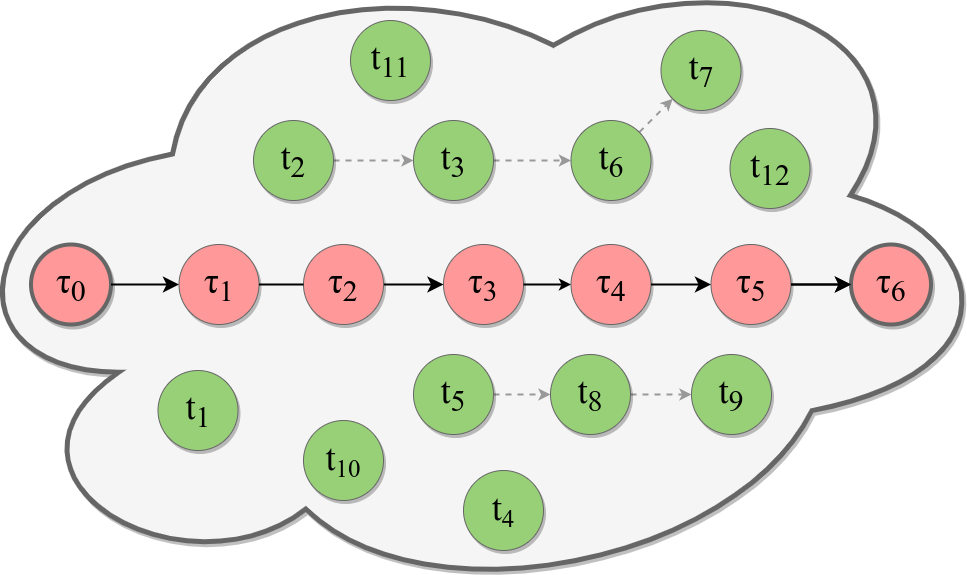
\includegraphics[width=0.8\linewidth]{schemas/SetDeTaches}
    		\caption{Représentation simplifiée du set de tâches à criticité duale}
    		\label{fig:SetdeTaches}
    	\end{figure}
    	
    	
    	\subsubsection{Modèle de tâches}
		La plupart des hypothèses faites ici se focalisent sur les tâches critiques, tandis que la seule hypothèse forte sur les tâches non critique est la capacité à les stopper (soit un arrêt total, soit une mise en pause) et les relancer en cours d'exécution de façon à pouvoir déclencher un Mode Dégradé où il n'y a plus de tâches non critiques avec les risques d'interférences afférents envers les tâches critiques. Sous les systèmes type Unix, cela correspond typiquement à l'envoi d'un signal SIGSTOP et SIGCONT. Sans cette condition, les Modes de Service mentionnés ci-dessus ne sont pas exploitables pour notre besoin. 
		
		Chaque tâche critique $\tau_i$ est activée et exécutée suivant une période $T_i$. 
		À chaque période, le job $\tau_{i,j}$ correspond à la $j^{ieme}$ exécution de la tâche $\tau_i$. 
		On peut alors noter pour chaque job $\tau_{i,j}$ son moment d'activation $a_{i,j}$, son début d'exécution $s_{i,j}$ et sa terminaison $e_{i,j}$. 
		On considère qu'un job consomme toutes ses données d'entrée (inputs) au début de son exécution, s'exécute et fourni à la fin de son exécution les données de sortie. Les données d'entrée et de sortie des tâches sont stockées en espace mémoire partagé : la transmission des données d'une tâche à l'autre se fait de façon asynchrone.
		Cela nous mène à la question de l'interaction entre les tâches et notamment la façon de représenter la précédence.
		%%%%%%%%%%%%%%%%%%
		%%\alert{Citer différents modèles d'exécution de tâches existants ici ? c.f. ~\cite{friese_estimating_2018}}
    	%%%%%%%%%%%%%%%%%%
    	
    	\subsubsection{Chaînes de tâches}
	    La question de la dépendance entre les tâches est importante pour aborder le problème des contraintes temps-réel avec une vision plus macroscopique. En effet, dans le cadre de l'usage de tâches ayant des contraintes temporelles souples (c.f.~\autoref{sec:SystemesTempsReels} - Systèmes temps-réel), c'est uniquement avec une vision plus globale de l'exécution du système qu'il est possible de tirer au maximum parti des légers dépassements pour éviter dans la globalité d'avoir recours à des politiques d'exécution des tâches plus restrictives, et par conséquent qui sous-exploitent la puissance de calcul disponible.
	    Nous considérons ici la dépendance entre les tâches via les données partagées entre ces dernières selon un modèle type producteurs/consommateurs. Les tâches ont des relations de cause à effet et par conséquent, d'un point de vue strictement fonctionnel on peut décrire le système comme étant une accumulation de fonctionnalités réalisées par l'exécution de tâches successives. Cela permet alors d'introduire la notion de contrainte temporelle fonctionnelle, qui décrivent des contraintes d'exécution de chaînes de tâches bout-en-bout.
	    
	    
	    On représente une dépendance entre tâches sous la forme de chaînes de tâches, suivant le modèle $\tau_{1} \rightarrow \tau_2 \rightarrow \ldots \rightarrow \tau_n$. Dans un tel exemple, $\tau_1$ est la \textbf{tâche d'entrée} de la chaîne, tandis que $\tau_n$ est la \textbf{tâche de sortie} de la chaîne. Notons que ce modèle peut être étendu pour supporter des tâches représentées par un Diagramme Orienté Acyclique (\textit{Directed Acyclic Graph - DAG}) sans difficulté. Nous travaillons dans le cadre de ces travaux avec des chaînes directes, sans divergences ou convergences dans le graphe. De fait, cet ajout de complexité dans le modèle de chaîne de tâches n'apportera pas de différences particulières sur les résultats ni sur la démarche. De fait la différence fondamentale étant sur la façon de monitorer et reconstituer l'état de la chaîne de tâches, ce sont des éléments qui sont modifiables simplement pour prendre en compte un DAG complet. Le reste du principe présenté demeure fondamentalement inchangé.

	    %%%%%%%%%%%%%%%%%%%%%%%%%%
	    %\alert{J'hésite à présenter ça dans "l'autre sens" : présenter un modèle de chaînes de tâches plus complet (avec divergences, convergences, etc.) et au final restreindre le modèle à des chaînes linéaires qu'au niveau du cas d'étude (chapitre 5). Option 2 (actuelle): en perspective de la thèse présenter les implications d'un modèle de chaînes plus complexe}
	    %%%%%%%%%%%%%%%%%%%%%%%%%%
	    \begin{figure}[ht]
	    	\centering
	    	\includegraphics[width=.8\linewidth]{Chronogram_TaskChain}
	    	\caption{Exemple d'exécution d'une chaîne de tâches $\tau_1 \rightarrow \tau_2 \rightarrow \tau_3$}
	    	\label{fig:chain_chronogram}
	    \end{figure}
    
	    Dans ce contexte, on définit à l'exécution la précédence entre les tâches par le biais d'un lien type producteur-consommateur. On considère que pour une tâche, les données produites sont disponibles à partir de la terminaison de cette dernière. Chaque tâche dans la chaîne de tâche consommera les données de sortie de tous les jobs de la tâche précédente dans cette chaîne qui n'ont pas encore été consommées au début de son exécution. En regardant l'exemple de la~\autoref{fig:chain_chronogram} avec une chaîne $\tau_1 \rightarrow \tau_2 \rightarrow \tau_3$, à considérer que chaque job est désigné par la notation $ \tau_{i,j} $, $i$ indiquant la tâche et $j$ l'indice d'occurrence d'exécution de cette tâche. On peut voir que le job $ \tau_{2,2} $ consomme les données de $ \tau_{1,1} $, mais pas celles de $ \tau_{1,2} $, étant donné que ce job n'est pas encore terminé à t=15. Aussi, $ \tau_{2,3} $ pourra consommer les données de $ \tau_{1,2} $ et $ \tau_{1,3} $ étant donné qu'elles n'ont pas été consommées précédemment.
	    
	    De façon formelle, on peut définir cette relation entre une tâche $\tau_i$ et son successeur $\tau_{i+1}$. Pour produire la donnée de sortie du job $\tau_{i+1,k}$ de la tâche $\tau_{i+1}$, ce dernier consommes toutes les données d'entrée en attente provenant des jobs $\tau_{i,j}$. Les données en attente étant celles qui n'ont pas été consommé par le job $\tau_{i+1,k-1}$ qui est le job précédent de $\tau_{i+1}$. On peut donc écrire que pour un $\{i,k\}$ donnés, sont consommés les données de tous les jobs $\tau_{i,j}$ tel que $ e_{i,j} \leq s_{i+1, k}$ et $e_{i,j} > s_{i+1, k-1}$. Autrement dit, un job $\tau_{i,j}$ n'a un effet sur $\tau_{i+1,k}$ si et seulement si ce dernier est le premier job de $\tau_{i+1}$ exécuté après la terminaison de $\tau_{i,j}$.
	    
	    \textbf{Remarque de compréhension} : \textit{les indices $j$ et $k$ ci-dessus représentent tous deux la différenciation des jobs pour une tâche donnée ($\tau_1$ pour $j$ et $\tau_2$ pour $k$). Si 2 lettres différentes sont utilisées, c'est uniquement du fait qu'il n'y a pas de relation entre 2 jobs de tâches différentes qui auraient le même indice d'occurrence. D'où la distinction $j$/$k$}.
	    
		Dans ces conditions, on nomme $\tau_{i+1,k}$ le \textbf{successeur} du job $\tau_{i,j}$. On note $succ()$ la fonction qui permet de trouver le successeur d'un job donné tel que~: 
		\begin{multline*}
		\forall i,j \in \mathbb{N}^*, \, \exists \, k \in  \mathbb{N}^*  \textrm{ tel que }  \\
		 succ(\tau_{i,j}) = \tau_{i+1,k} \textup{ avec } e_{i,j} \leq s_{i+1,k} \wedge e_{i,j} > s_{i+1,k-1}
		\end{multline*}
	
		Par extension, la fonction itérative $succ^{p}()$ pour tout $p \geq 0$ permet de trouver le p\up{ème} job successeur d'une tâche donnée de la chaîne de tâches. Et in fine, $succ^{n-1}(\tau_{1,j})$ désigne le job de sortie de la chaîne de tâche désignée par son job d'entrée $\tau_{1,j}$. On notera que pour $p = 0$, on définit $succ^{\,0}(\tau{i,j}) = \tau_{i,j}$, soit la fonction identité.
		
		Pour illustrer cela, on peut reprendre l'exemple de la chaîne représentée en~\autoref{fig:chain_chronogram}. On peut par exemple voir qu'une des exécutions de la chaîne de tâche, débutant par $\tau_{1,1}$, donne : $succ^{2}(\tau_{1,1}) = succ(succ(\tau_{1,1})) = succ(\tau_{2,2}) = \tau_{3,2}$. Mais aussi que le job $ \tau_{2,3} $ doit prendre en compte les valeurs de sorties de 2 jobs de la tâche $ \tau_1 $. Plus précisément, $succ(\tau_{1,2}) = succ(\tau_{1,3}) = \tau_{2,3} $. %On a alors le temps de réponse de la-dite chaîne : $R_1 = e_{3,2} - s_{1,1} = 31 - 5 = 26$ unités de temps.
		En effet, étant donné que les tâches peuvent être définies par des périodes d'activation différentes, cela signifie notamment que si une tâche $\tau_i$ est exécutée plus fréquemment que son successeur $succ(\tau_{i+1})$, alors il est possible  qu'un job $\tau_{i+1,j}$ soit le successeur de plusieurs jobs de la tâche $\tau_{i}$.
		
		Par extension et commodité d'usage, on ajoutera comme notations utiles $succ(a_{i,j}), \quad succ(s_{i,j}), \quad succ(e_{i,j})$ respectivement les temps d'activation, de début d'exécution et de terminaison du successeur du job $\tau_{i,j}$. Et de même par fonction itérative, $succ^k(s_{i,j})$ la date de début du k\up{ième} successeur de la tâche $\tau_{i,j}$~: 
		
		\begin{align*}
%%			\textup{Soit } succ(\tau_{i,j}) = \tau_{i+1,k} \textup{, alors :}	\\
		\textup{Soit } succ(\tau_{i,j}) = \tau_{i+1,k} \textup{, alors }
			succ(a_{i,j}) = a_{i+1,k} 	\\
			succ(s_{i,j}) = s_{i+1,k}	\\
			succ(e_{i,j}) = e_{i+1,k}	\\
		\textup{De même, si } succ^n(\tau_{i,j}) = \tau_{i+n,k} \textup{ alors }
			succ^n(a_{i,j}) = a_{i+n,k}		\\
			succ^n(s_{i,j}) = s_{i+n,k}		\\
			succ^n(e_{i,j}) = e_{i+n,k}
		\end{align*}
	    
  		 Cette façon de considérer les choses permet une plus grande flexibilité de notre modèle pour s'adapter à un cas concret. De cette façon le modèle gère déjà un nombre assez significatif d'implémentations de tâches existantes~:
	\begin{itemize}
		\item   		Des tâches avec une file d'attente en entrée : lorsque la tâche est exécutée elle consomme toutes les données d'entrée en attente -- le cas de base que nous considérons.
		\item   		Des tâches qui ne consomment que la donnée d'entrée la plus récente, les données précédentes étant considérées obsolètes. Dans ce cas-là, c'est équivalent à considérer que toutes les données précédentes sont consommées, mais qu'uniquement la plus récente est prise en compte, celle des jobs plus anciens sont ignorées.
		\item   		Pour les tâches où chaque exécution de la tâche ne prend en compte qu'une seule donnée en file d'attente, notre modèle ne gère pas tous les cas. Cela peut être la donnée la plus ancienne (stratégie FIFO\footnote{FIFO : First-In First-Out, les données sont traitées de la première arrivée à la dernière.}) ou la plus récente (stratégie LIFO\footnote{LIFO : Last-In First-Out, les données sont traitées de la dernière (plus récente) arrivée à la plus ancienne.}). Quoi qu'il en soit, notre capacité à prendre en compte ce type de tâche va être dépendant de leur fréquence d'activation. 
		\begin{enumerate}
			\item 	Si les tâches s'exécutent toutes à la même fréquence, alors il y aura systématiquement une relation 1\string:1 entre producteurs et consommateurs.
			\item 	Si les tâches successeur dans une chaîne donnée s'exécutent systématiquement à une plus grande fréquence que les tâches précédentes, alors nous sommes aussi dans un cas avec jamais plus d'une donnée disponible en file d'attente. En effet, la tâche Consommateur s'exécutant plus rapidement que la Tâche productrice, le ratio Production/Consommation est inférieur à 1.
		
		Ces 2 cas sont donc équivalents au premier type de tâches mentionné pour lequel toutes les données produites sont consommées, mais où la quantité de données en attente est systématiquement inférieure ou égale à 1 en réalité.
			\item 	En revanche si une tâche successeur dans une chaîne s'exécute plus lentement que sa prédécesseure, c'est le cas qui n'est pas géré par ce modèle. En effet, si une seule donnée est consommée par job, et le reste stocké en file d'attente, alors il pourrait y avoir un ratio Production/Consommation supérieur à 1. C'est-à-dire une plus grande quantité de données produites que consommées. Ce cas est relativement improbable (à moins d'une erreur de conception), car cela implique que la quantité de données en file d'attente peut potentiellement diverger. Or la file d'attente ne peut être considérée infinie.
		\end{enumerate}  
	\end{itemize}
  		De façon succincte, quand on parle de consommer plusieurs jobs de la tâche précédente tel qu'on le présente ici, cela n'implique pas que toutes ces données seront prises en compte. Tout dépend du modèle de fonctionnement interne des tâches. Mais quoi qu'il en soit, cela permet de gérer un grand nombre de comportements classiques.
  		
  		Nous ne considérons pas dans notre modèle d'éventuels délais entre l'instant où une tâche produit sa donnée de sortie et le moment où cette donnée est réellement disponible pour la ou les tâches consommatrices. Il faudrait pour cela ajouter dans notre modèle de précédence une constante de latence correctement estimée selon l'implémentation de la transmission des données entre les tâches. On pourra noter sur ces aspects les travaux de~\cite{friese_estimating_2018} qui ont pu aborder la prise en compte de latences dans différents modèles de chaînes de tâches.


        \paragraph{Temps de réponse bout-en-bout}

    La notion de successeur permet de définir le temps de réponse bout-en-bout $R_j$ de la $ j $-ème instance d'exécution d'une chaîne de tâche. Ainsi $R_j$ désigne le temps écoulé entre l'activation du \textit{job} d'entrée $\tau_{1,j}$ de la chaîne, jusqu'à la terminaison du \textit{job} de sortie $\tau_{n, k} = succ^{n-1}(\tau_{1,j})$.
    On a alors $R_{j} = succ^{\,n-1}(e_{1,j}) - a_{1,j}$ que l'on peut retrouver dans l'exemple du~\autoref{fig:chain_chronogram}. Sur cet exemple, il est possible de reconstituer trois instances d'exécution de la chaîne de tâches avec les trois temps de réponse correspondants : $R_1$, $R_2$, $R_3$. 
    %Parmi ces instances, on remarque que 2 d'entre-elles sont très semblables, avec le même job de terminaison $ \tau{3,3} $.
    
	Intuitivement, l'échéance bout-en-bout représente alors la durée maximale acceptable pour qu'une donnée d'entrée de la chaîne ait un effet du côté de la sortie. Pour une fonctionnalité donnée on comprend bien que cette échéance doit être bornée, et qu'il faut donc des garanties pour que tout se passe bien de bout-en-bout. Lorsque l'on considère l'échéance d'une chaîne de tâches $D_c$, pour éviter toute faute temporelle de non-respect d'échéance, il faut a minima respecter~:  $\max_{j \in \mathbb{N}}\{R_j\} \leq D_c$.
	
	\smallbreak 
	
	L'objectif à présent est de proposer une approche qui permette justement d'exploiter ces contraintes bout-en-bout, de façon à éviter les risques de fautes temporelles au niveau fonctionnel. Cela se traduit par la volonté de prévenir les risques de dépassement d'échéances, non pas au niveau de chaque tâche individuelle, mais plutôt à un niveau d'observation au-dessus qui est en lien direct avec la représentation fonctionnelle.
	
    
\section[Mécanisme d'anticipation]{Mécanisme d'anticipation \\ par Surveillance et Contrôle}
    \subsection{Méthode d'anticipation}
    
    Je propose donc un mécanisme basé sur la surveillance à l'exécution de l'avancement d'une chaîne de tâche. 
    Pour ce faire, on introduit les notions d'\textbf{État de Chaîne de Tâche} et de \textbf{Trace d'Exécution de Chaîne de Tâche}. Une chaîne de tâches donnée est associée à un État et plusieurs Traces d'Exécutions. Ces deux éléments évoluant au fil de l'exécution du système, on peut noter $S(t)$ l'État à l'instant t et $ET(j,t)$ la j\up{ème} Trace d'Exécution de la Chaîne de tâches à l'instant t.
    
    On peut alors définir pour une Chaîne de Tâches dont la tâche d'entrée est $\tau_{1}$, et la tâche de sortie $\tau_{n}$ : 
    \begin{definition} \label{def:TraceExecutionChaine}
    	Une \textbf{Trace d'Exécution} $ET(j,t)$ se définit par le début d'exécution d'un job d'entrée $s_{1,j}$ ainsi que tous les temps de fin d'exécution $e_{i,j}$ des \textit{successeurs} itératifs de ce job qui ont été identifiés à l'instant $t$.
    	\begin{equation*}
    		ET(j,t) = \{\: a_{1,j} \:,\: e_{1,j} \:, succ(e_{1,j})\:, \;\dots\; ,\: succ^{n-1}(e_{1,j}) = e_{n,k} \:\}
    	\end{equation*}    	
    	Une Trace d'Exécution $ET(j,t)$ est dite \emph{active} si son job de départ $\tau_{1,j}$ a déjà été activé à l'instant t, et que son successeur itératif correspondant à la tâche de sortie de la chaîne $\tau_{n,k}$ n'a pas encore été terminé. Autrement, elle est \textit{inactive}. En d'autres termes :
    	\begin{equation*}
    		ET(j,t)  \quad \textrm{est active ssi}\quad  a_{1,j} \leq t \quad \textrm{et} \quad e_{n,k} > t
    	\end{equation*}
    \end{definition}
    
    %Our anticipation mechanism is based on the run-time monitoring of the task chain progress. 
    %To that end, we introduce the notions of \textbf{Task Chain State} and \textbf{Task Chain Execution Trace} (TCET). 
    %A TCET contains an entry task job and all the iterative successors of that job. 
    %At a time $t$ a TCET can be \emph{active}, if its entry task job has been activated and if its exit task job has not yet ended, or \emph{inactive} otherwise. 
    
    Il est possible de définir à partir des Traces d'exécution, actives ou inactives à un instant $t$, l'État de la Chaîne de tâches :
    
    \begin{definition}\label{def:EtatChaine}
    	L'\textbf{État d'une Chaîne de Tâches} $S(t)$ défini à un instant $t$ l'état d'avancement de l'exécution de la chaîne de tâches qui est toujours en cours et qui a été activée la plus anciennement. Autrement dit, $\pmb{S(t) =\langle t_0, \tau_p\rangle}$ basé sur la Trace d'Exécution la plus ancienne active $ ET(j,t) $ tel que~:
    	\begin{equation*} 
    		\left|
			\begin{array}{ll}
				\displaystyle	t_0 &= \displaystyle\min_{j \in \mathbb{N}^*} \left\{ a_{1,j} \mid
			    	  					a_{1,j} \leq t \wedge succ^{n-1}(e_{1,j}) > t \right\}		\\
			    \displaystyle	\tau_p = succ^{\,p}(\tau_{1,j}) &= \displaystyle\min_{l\,\in\,[\![0;n-2]\!] } \left\{ succ^{\,l+1}(\tau_{1,j}) \mid succ^{\,l}(e_{1,j}) \leq t \right\}
			\end{array}
    	  	\right.
    	\end{equation*}
    Avec $t_0$ la plus ancienne activation parmi les $ET(j,t)$ et $\tau_p$ la prochaine tâche de cette trace d'exécution qui n'a pas encore été terminée.
    \end{definition}

    De cette façon, l'État d'une chaîne de tâches indique quelles sont les tâches restantes à exécuter dans la chaîne à un instant donné et son temps de réponse partiel actuel que l'on notera $RT(t) = t - t_0$. Et l'état de la chaîne se focalise sur la chaîne active la plus ancienne, donc la plus longue ce qui implique que c'est la plus à même de dépasser l'échéance.
    
    Pour finir, au regard de l'État d'une chaîne de tâches, on peut s'intéresser au temps restant jusqu'à la complétion de cette chaîne. Il est possible d'estimer le temps qu'il faudra pour aller jusqu'à exécuter la tâche de sortie de la chaîne qui fait partie de la Trace d'Exécution active observée, c'est-à-dire $succ^{\,n-1}(\tau_{1,j}) = \tau_{n,j}$. Et si, de plus, cette estimation est faite dans les hypothèses d'estimation de Temps d'Exécution Pire Cas, on obtient alors une estimation de \textbf{\emph}{Pire Temps de Réponse restant} $rWCRT(t)$ à l'instant $t$ pour terminer l'exécution de la trace d'exécution active la plus longue.
    
    Alors, en combinant l'État à un instant $t$ avec une estimation du Temps de Réponse Pire Cas restant, on peut donc estimer une borne haute garantie de temps de réponse de la chaîne de tâche. C'est là que l'on peut faire entrer en jeu un mécanisme d'anticipation. 
    On dispose pour une chaîne de tâches donnée de son temps de réponse partiel actuel ainsi qu'une estimation de temps de réponse restant en pire cas. Il est alors possible de déterminer s'il y a un risque de défaillance par dépassement de l'échéance bout-en-bout $D_c$.
    \begin{theorem}[Risque de dépassement d'échéance]
    	Si à un instant donné $t$, l'inéquation suivante est respectée, alors il y a risque de dépassement d'échéance.
    	\begin{equation*} 
    		RT(t) + rWCRT(t) > D_c
    	\end{equation*}
    \end{theorem}

	Pour illustrer cette logique, on peut voir sur le chronogramme~\ref{fig:chronogram_rWCRT_example} à nouveau un exemple avec une chaîne de tâches $\tau_1 \rightarrow \tau_2 \rightarrow \tau_3$. À l'instant $t=18$ d'indiqué il y a deux Traces d'Exécution actives (chaînes reliées par une flèche de succession). On a de ce constat l'État de la chaîne $S(t) = \langle \tau_0, \tau_2\rangle = \langle 5, \tau_{2} \rangle $.
	On en déduit $ RT(18) = t - t_0 = 18-4 = 14 $. Si l'on ajoute à cela une estimation du Temps de Réponse Pire Cas restant $rWCRT(18)$, qui est le temps estimé pour que $\rightarrow \tau_2 \rightarrow \tau_3$ soit exécuté selon les contraintes de précédence, alors on a l'estimation du Pire Temps de Réponse : $ RT(18) + rWCRT(18) = 33$ que l'on peut comparer à la date d'échéance $ D_c = 30 $. Dans cet exemple, il existe donc un risque de dépassement de l'échéance.
	Il est à noter aussi que dans cet exemple l'instant $t$ a été pris en plein pendant l'exécution de la tâche $ \tau_2 $. Ce qui est pris en considération comme si cette dernière n'était pas exécutée. Si l'on ne prend pas non plus en compte son exécution partielle, c'est parce que d'un point de vue externe à cette tâche, sans l'instrumentaliser il n'est pas possible de le savoir. Et de fait, l'une de nos contraintes étant d'être le moins intrusif possible sur le code, notamment pour les cas où certains logiciels ne sont pas modifiables (black-box ou legacy). 
	
    \begin{figure}[ht]
		\centering 
		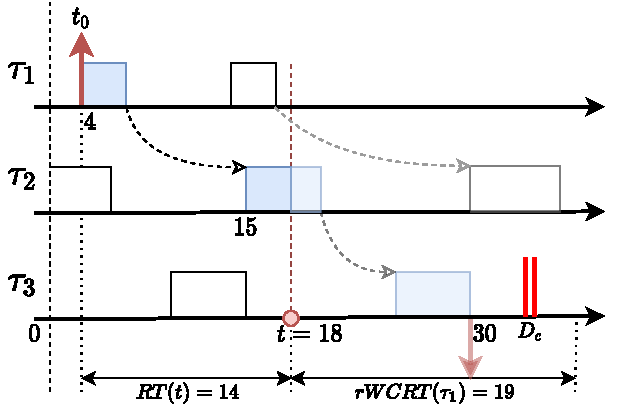
\includegraphics[width=0.7\linewidth]{chronogram_rWCRT_example.pdf}
		\caption{Chronogramme de calcul du risque de dépassement à un instant t}
		\label{fig:chronogram_rWCRT_example}
	\end{figure}

	À présent, il faut nous souvenir de notre objectif dans tout cela. Pourquoi vouloir anticiper une défaillance de la sorte ? L'objectif est d'anticiper un risque de dépassement d'échéance à l'échelle d'une chaîne de tâches, de façon à pouvoir passer d'un Mode d'ordonnancement Nominal vers un mode Dégradé dans lequel on va prévenir la défaillance. Cette dernière a pour origine première les interférences matérielles qui augmentent les temps d'exécution des tâches. Aussi pour éviter davantage ce glissement temporel et donc conserver la garantie de terminaison de la chaîne de tâches avant l'échéance, on remonte à la source en prévenant temporairement tout risque d'interférences. Et cela est obtenu via un mode dégradé dans lequel la méthode consiste à stopper temporairement les tâches non critiques, cause des interférences.
	Il nous faut décrire à présent la méthode de passage en mode dégradé.
	

    
    \subsection{Passage en Mode Dégradé}
    
        \paragraph{Estimation de Temps d'Exécution Pire Cas restant}
    Bien évidemment, l'estimation du Temps de Réponse Pire Cas restant est un élément clé de l'approche. Tout l'intérêt de cette méthode réside dans la capacité à passer dans un mode dégradé. En conséquence, ce que nous nous devons de garantir, c'est le non-dépassement d'échéance sachant qu'il est possible à tout moment de prendre la décision du passage en mode dégradé, dans lequel les tâches critiques n'étant plus sujettes à interférences externes, auront un Temps d'Exécution Pire Cas bien plus faible qu'en mode Nominal. 
    Cela implique directement que si le $rWCRT(t)$ que nous considérons est dans le contexte Dégradé, alors la détection d'un éventuel risque se fait de façon beaucoup plus permissive que si l'on considère directement les risques en mode Nominal. 
    Étant donné que le mode dégradé correspond à un arrêt des tâches non critiques, on peut considérer que dans ce mode la chaîne de tâches est en isolation. De ce fait, la seule chose qui va modifier l'estimation du $rWCRT(t)$ va être l'État de la chaîne de tâches à l'instant t, $S(t)$. Or, étant donné que $S_c = \langle t_0, \tau_i\rangle$, alors on remarque qu'il n'y a que la valeur de $\tau_i$ -- c'est-à-dire la prochaine tâche de la chaîne qui doit être exécutée -- qui va influer sur la valeur estimée du pire temps de réponse restant. Ainsi, $rWCRT(t)$ peut être simplifié en une fonction discrète qui évolue avec $S(t)$. Par conséquent, on notera pour la suite de notre raisonnement $rWCRT(t) = rWCRT(\tau_i)$. 
    
    Ceci étant posé, il existe plusieurs méthodes à l'estimation de $rWCRT(\tau_i)$. 
    De façon théorique, il est possible d'exploiter les méthodes déjà existantes d'estimation de temps d'exécution pire cas, auxquelles il faut ajouter la prise en compte des temps d'activation des tâches. Ce type d'approche devient hautement dépendante du système étudié, que ce soit l'architecture matérielle, mais surtout la politique d'ordonnancement des tâches, le type de tâches (périodique, sporadique, interruption)... De façon générale, la complexité des approches théoriques n'est pas négligeable et, il faut l'admettre, hors de notre cadre d'expertise. C'est d'autant plus vrai dans un cas d'application sur processeur multicœur pour lequel il est facile de tomber dans des estimations trop pessimistes. Pour cette raison, nous avons décidé dans notre proposition d'avoir une approche plus expérimentale.
    
    %To help with the estimation of $rWCRT$, we assume that the HI-criticality task chain execute on a single core. To avoid interference between the MCA and the task chain we prevent the MCA to use the same core. Lo-criticality tasks can execute on any core as depicted on \autoref{fig:SoftwareArchitecture}. 

    Un avantage dont nous bénéficions ici, c'est que l'hypothèse de se ramener à un cas en isolation dans le mode dégradé limite grandement les risques de variations sur les temps d'exécutions des tâches critiques. C'est ce qui permet une plus grande certitude sur les estimations expérimentales, qui ne nécessitent alors plus de couvrir toute une combinatoire incluant les tâches non critiques. L'estimation est donc faite expérimentalement en exécutant le système avec un passage forcé en mode dégradé dans lequel on peut alors mesurer sans les tâches non-critiques les Temps de Réponse Pire Cas restants $rWCRT(\tau_i)$. On notera que pour une chaîne de N tâches, il y a N-1 $rWCRT$ à estimer. Plus de détails sur le protocole adopté pour l'estimation seront abordés en~\autoref{chap:4_ProtocolExpe}.

    La transition en elle-même vers le mode dégradé est une phase importante du fait qu'elle implique des délais supplémentaires qui devront être pris en compte dans l'anticipation. De cette façon, à considérer que l'on recalcule périodiquement le risque de dépassement d'échéance, il est possible de définir l'instant où l'on sait que l'attente d'une période supplémentaire va faire que même en mode dégradé, il ne sera plus possible de garantir le respect de l'échéance bout-en-bout. Par conséquent, il devient alors clair que cet instant-là devient le dernier moment auquel il faut nécessairement passer en mode dégradé pour justement conserver cette garantie.

%The MCA role is first to monitor the state of a HI-criticality task chain to detect potential deadline miss. If such a potential fault is anticipated, then the MCA switches the system to HI-criticality mode, pausing all non essential workload (LO-criticality tasks), to prevent further interference on the HI-criticality tasks and allow a safe termination. To be efficient, the switch  must be triggered only when necessary (as a “mode switch procrastination”, as called in~\cite{hu_ffob_2019}). That is why we also focus on end-to-end deadline, rather than individual task deadlines, in order to avoid false-positive switching, meaning switching to HI-criticality mode although there is slack in the task chain. Indeed, with an end-to-end perspective, we can use the slack given by a task finishing early to compensate the lateness of an other task in the chain.

	\paragraph{Transition de Mode}
    Ce changement de mode se fait en 3 étapes. Il faut en premier lieu bien entendu la détection du point de bascule auquel le risque de défaillance est détecté, c'est l'étape de décision. Une fois la décision prise, la seconde étape est d'activer le mécanisme de passage en mode dégradé. Dans notre cas, il s'agit d'envoyer un signal aux tâches non critiques de façon à mettre en pause leur exécution, c'est l'étape de contrôle. Enfin, le système de surveillance doit continuer d'observer l'État de la chaîne de tâches de façon à relancer les tâches non critiques une fois le risque passé. Il s'agit de l'étape de recouvrement.
    
    Ces trois étapes font ressortir un élément important pour l'anticipation qui n'a pas été pris en compte pour le moment, et il s'agit de la durée entre l'étape de décision et la fin de l'étape d'exécution. En effet, le temps pour que toutes les tâches non critiques soient mises en pause est non nul, et ce délai doit être pris en compte dans l'estimation de Temps d'Exécution Pire Cas restant. %dans l'optique où le pire cas en question est considéré dans le mode dégradé.
    
	En conclusion, en considérant les grandeurs suivantes : 
	\begin{itemize}
		\item 	$ W_{MAX} $ La durée maximum garantie entre 2 points de surveillance de l'Etat de la chaîne de tâche
		\item 	$ t_{SW} $ Le délai maximum nécessaire à la transition du mode nominal au mode dégradé
		\item 	$ rWCRT(\tau_i) $ pour chaque $\tau_i$ de la chaîne de tâche, les Temps de Réponses Pire Cas restant en mode dégradé
	\end{itemize}
	Il est alors possible de calculer la somme du temps de réponse partiel actuel avec ces trois métriques. Tant que cette somme reste inférieure à l'échéance bout-en-bout, alors on peut conserver le système en mode nominal. En revanche, à partir du moment où cela dépasse l'échéance, alors c'est le moment où il n'est plus sûr de rester en mode nominal, et il faut donc déclencher le mode dégradé pour garantir le respect de l'échéance. Cela correspond en conséquence à surveiller que l'inéquation suivante reste vraie pour savoir l'instant critique auquel il faut passer en mode dégradé~:
	\begin{equation} \label{eq:safe_cond}
		RT(t) + rWCRT(\tau_i) + W_{max} + t_{SW} \leq D_c
	\end{equation} 
	Cette équation est notamment adaptée des travaux de~\cite{kritikakou_run-time_2014}. Chaque point de surveillance de l'État de la chaîne de tâches est considéré comme étant temporellement sûr (au sens où il n'y a pas de risque de faute temporelle due au dépassement d'échéance) tant que cette inégalité est respectée.
    
    \begin{proof}
		En présumant que (\ref{eq:safe_cond}) est respectée, on peut montrer qu'il est sûr d'attendre le prochain point de surveillance pour décider de changer de mode. \nline
		À l'instant de surveillance $t$, soit $t_{next}$ le prochain instant de surveillance.\nline
		Par définition, $t_{next} \leq t + W_{max}$. Alors $RT(t_{next}) \leq RT(t) + W_{max}$. 
		Par conséquent, \smallbreak
		$RT(t_{next}) + rWCRT(\tau_i) + t_{SW} \leq RT(t) + rWCRT(\tau_i) + W_{max} + t_{SW}$. \nline
		Aussi, $rWCRT()$ ne peut que décroître avec le temps qui s'écoule. Par conséquent, %\smallbreak
		\[ rWCRT(t_{next}) \leq rWCRT(\tau_i)	\]
		et 
		\[ RT(t_{next}) + rWCRT(t_{next}) + t_{SW} \leq RT(t) + rWCRT(\tau_i) + W_{max} + t_{SW} \] 
		Étant donné que (\ref{eq:safe_cond}) est respecté, on a $RT(t_{next}) + rWCRT(t_{next}) + t_{SW} \leq D_c$.
		De ce fait, il sera sûr de passer en mode dégradé au prochain point de surveillance.  
    \end{proof}
    
%    \begin{figure}[ht]
%    	\centering
%    	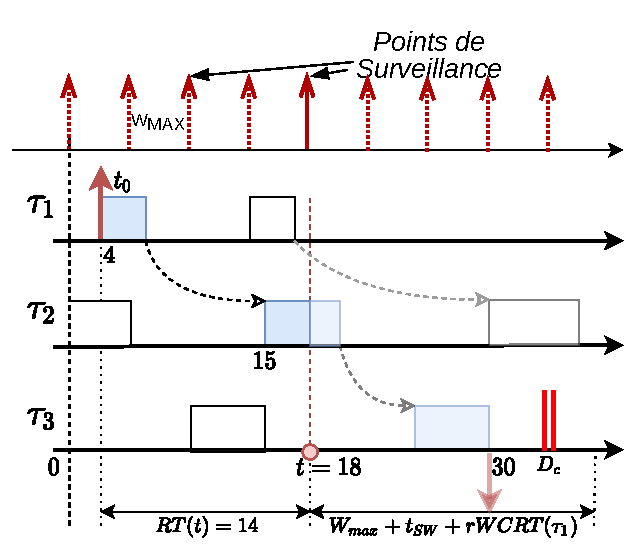
\includegraphics[width=0.92\linewidth]{schemas/chronogram_rWCRT_complet}
%    	\caption{Anticipation de défaillance par changement de mode}
%    	\label{fig:rwcrtchronogram}
%    \end{figure}
	\begin{figure}[ht]
		\centering
		\begin{subfigure}{0.7\textwidth} \centering
			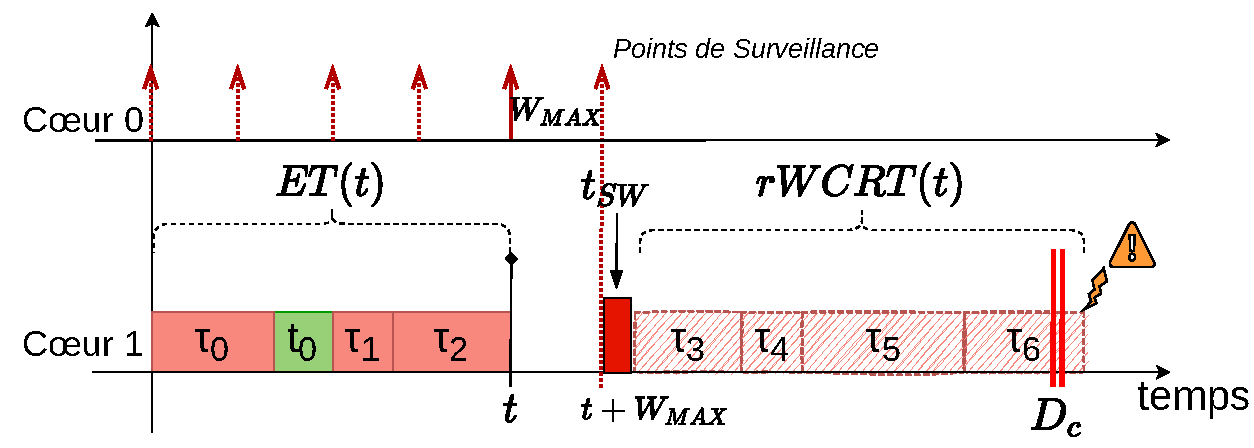
\includegraphics[width=\linewidth]{Chronogrammes-Anticipation_Defaillance}
			\caption[Anticipation - risque de défaillance]{Anticipation - calcul du risque de défaillance}
			\label{sufig:chrono_risque_defaillance}
		\end{subfigure}
		\begin{subfigure}{0.7\textwidth} \centering
			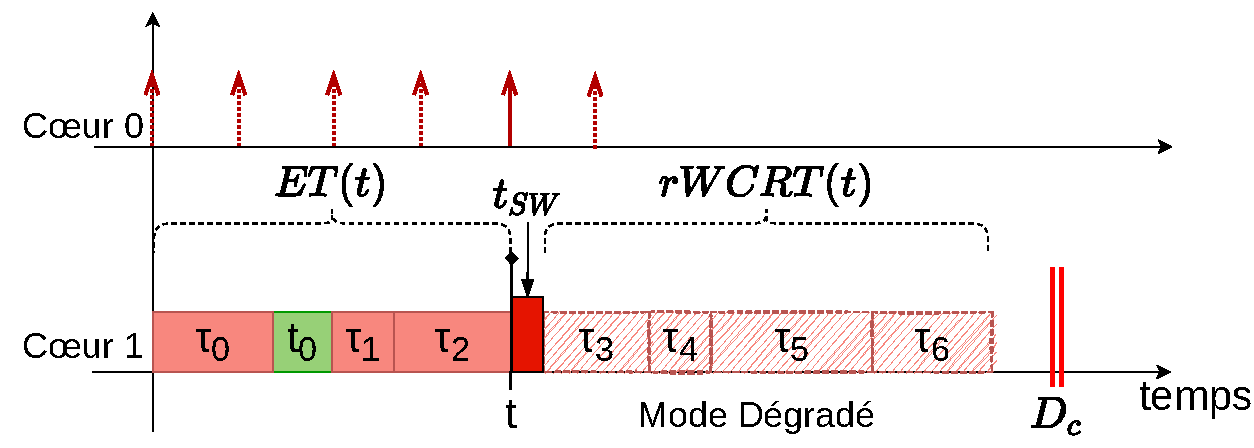
\includegraphics[width=\linewidth]{Chronogrammes-Anticipation_Corrigee}
			\caption[Anticipation - passage en mode dégradé]{Anticipation - déclenchement du passage en mode dégradé}
			\label{sufig:chrono_risque_ModeDegrade}
		\end{subfigure}
		\caption{Chronogrammes de fonctionnement du mécanisme d'anticipation}
		\label{fig:rwcrtchronogram}
	\end{figure}

    En conclusion, grâce au calcul d'anticipation de risque de dépassement d'échéance, il nous est possible d'identifier l'instant $t$ auquel il est nécessaire de passer en Mode Dégradé. La démarche que suit notre mécanisme d'anticipation est illustré en~\autoref{fig:rwcrtchronogram} avec l'hypothèse d'une chaîne de tâche~:
    \[  \tau_{1} \rightarrow \tau_{2} \rightarrow \tau_{3} \rightarrow \tau_{4} \rightarrow \tau_{5} \rightarrow \tau_{6} \] 
     
     À chaque point de Surveillance, le mécanisme anticipe le risque en calculant l'inégalité \ref{eq:safe_cond} comme reconstitué en~\autoref{sufig:chrono_risque_defaillance}. Si l'inégalité n'est plus respectée et donc que le risque est manifeste comme sur le chronogramme, alors le passage en mode dégradé est effectué, de façon à ce que ce soit le scénario représenté en~\autoref{sufig:chrono_risque_ModeDegrade} qui se réalise, et donc éviter le dépassement d'échéance potentiel. On notera la présence de la tâche non critique $t_0$ qui s'exécute sur le même cœur mais n'influe pas sur le calcul d'anticipation qui est fait.
	%La méthode de réglage de la période de surveillance sera discuté dans le~\autoref{chap:4_ProtocolExpe}.
	
	\section{Architecture Logicielle}
	
	Maintenant que nous avons présenté toute la logique derrière le mécanisme de surveillance et de contrôle, nous allons présenter plus en détail l'architecture logicielle nécessaire à son implémentation.
	
	Pour résumer, nous sommes dans le cas d'un système à criticité mixte implémenté sur un calculateur multicœur, dans lequel nous avons distingué une chaîne de tâches critiques des autres tâches considérées non-critiques. Nous souhaitons ajouter un Agent de Surveillance et de Contrôle pour assurer la fonctionnalité de mitigation des fautes temporelles sur la chaîne de tâches critique. Ce dernier se destine à être exécuté en couche bas niveau, au même niveau que la politique d'ordonnancement du système. Dans le cadre de la suite de nos expérimentations, pour simplifier l'implémentation, nous avons considéré l'isolation de l'Agent de Surveillance et Contrôle sur un cœur du processeur. L'ensemble de ces éléments se résume en~\autoref{fig:SoftwareArchitecture}.

	\begin{figure}[ht]
        \centering
        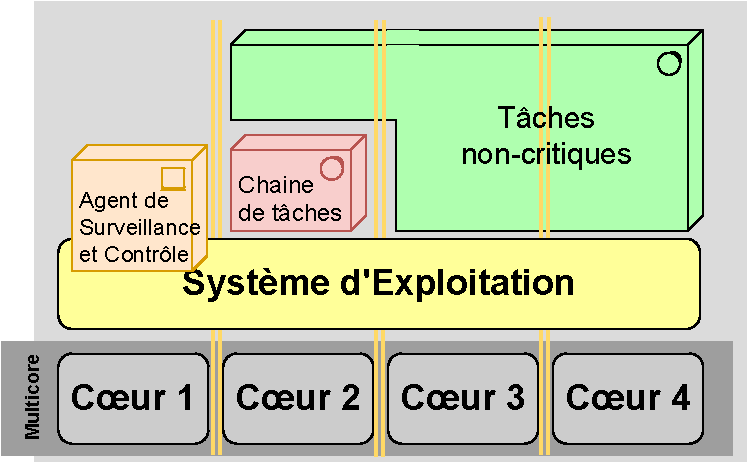
\includegraphics[width=.6\linewidth]{ArchitectureLogicielle.pdf}
        \caption{Architecture Conceptuelle du mécanisme de Surveillance et Contrôle} \label{fig:SoftwareArchitecture}
	\end{figure}

	L'Agent de Surveillance et Contrôle peut se décomposer en deux éléments distincts. D'un part un \emph{Task Wrapper Component} (TWC) et de l'autre le \emph{Core Control Component} (CCC). Le TWC se destine à récupérer toutes les informations nécessaires à la surveillance et la mise à jour de l'État de la Chaîne de tâches par le biais d'une encapsulation des tâches , tandis que le CCC doit prendre en compte ces informations, de façon à réaliser la prise de décision du passage en mode dégradé au regard de l'inéquation~\ref{eq:safe_cond}. Les interactions entre les différents composants logiciels sont représentées sur la~\autoref{fig:architecture}.
	
	
        \begin{figure}[ht!]
            \centering
            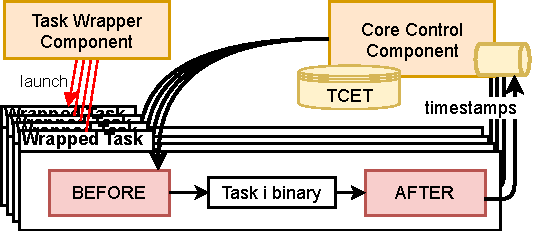
\includegraphics[width=0.7\linewidth]{ArchitectureFramework.pdf}
            \caption{Architecture Logicielle de l'Agent de Surveillance et Contrôle}
            \label{fig:architecture}
        \end{figure}
        
        
        \subsection{Task Wrapper Component (TWC)} 
        
        L'objectif du Task Wrapper Component est de gérer l'aspect Surveillance du mécanisme. Il englobe l'instrumentation du logiciel de façon non intrusive pour obtenir les informations nécessaires à la Surveillance. C'est une différence assez importante avec bon nombre de travaux qui se basent sur la surveillance de l'exécution de tâches. Souvent ces dernières reposent sur une instrumentation logicielle au niveau du code des tâches. Cela offre un suivi plus fin, mais avec un coût de développement logiciel supplémentaire pour chaque tâche. De plus c'est par définition incompatible avec du logiciel fourni en boite noire.
        
        Le mécanisme de Surveillance et Contrôle nécessite \begin{enumerate*}[label=\bfseries\alph*)]
        	\item une connaissance des dates d'activation et de terminaison des jobs, ainsi que 
        	\item la connaissance de la structure de la chaîne de tâche
        \end{enumerate*}. Concernant le premier point, il faut donc ajouter des blocs de code exécutés directement avant le début d'exécution des tâches ainsi que juste avant leur terminaison. En récupérant les \textit{timestamps}\footnote{timestamp~: en informatique, le temps se mesure par un compteur, une variable qui s'incrémente à la fréquence de fonctionnement du processeur. Un timestamp correspond à un horodatage sur ce compteur} d'exécution de ces blocs de code, il est ainsi possible de connaître précisément les dates de début $s_{i,j}$ et de fin $e_{i,j}$ de chaque job. Ils ont vocation à être envoyés au Core Control Component pour mettre à jour l'État de la chaîne de tâches ainsi que le suivi des Traces d'Exécution actives.
        
        Par ailleurs, une telle instrumentalisation permet d'ajouter une couche de sécurité supplémentaire. En effet, le changement de mode se fait initialement par envoi d'un signal pour stopper les tâches non critiques. Ceci étant dit, pour une meilleure réactivité et ajouter de la redondance dans l'arrêt des tâches, il est aussi possible d'utiliser le bloc logiciel exécuté avant l'exécution des tâches non critiques pour vérifier si la tâche en question a effectivement l'autorisation de s'exécuter ou bien si on est en mode dégradé, doit être stoppée. 
        
        En somme, le Task Wrapper Component doit encapsuler les tâches pour ajouter deux wrappers : un \textbf{Before} et un \textbf{After} qui vont avoir deux rôles : 
        \begin{itemize}
        	\item envoyer au Core Control Component les timestamps d'exécution associés à chaque job de tâche critique (dates de début et de fin),
        	\item ajouter de la redondance pour prévenir l'exécution des tâches non-critiques en mode dégradé et potentiellement accélérer le changement de mode.
        \end{itemize}
		On remarquera qu'il n'est pas utile d'exécuter un wrapper After à la suite des tâches non critiques étant donné que nous ne monitorons pas leur exécution dans le cadre du mécanisme.

        \subsection{Core Control Component (CCC)}
        
        Le Core Control Component gère donc l'aspect "Contrôle" du mécanisme. Il doit être exécuté périodiquement, tous les $T_{CCC}$ unités de temps. À chaque exécution, son rôle est de récupérer toutes les données de timestamps du TWC. En ayant connaissance de la structure de chaîne de tâches qui est exécutée, il peut alors reconstruire les Traces d'Exécution telles que définies précédemment (Définition~\ref{def:TraceExecutionChaine}). 
        
        À partir des Traces actives, l'État de la chaîne de tâches $S(t)$ est alors mis à jour. Il s'agit de calculer successivement : 
        \begin{itemize}
        	\item $RT(t)$, la durée à partir de la date de départ de la tâche d'entrée,
        	\item $rWCRT(\tau_i)$, le Temps de Réponse Pire Cas restant à prendre en compte selon l'état de la trace d'exécution active.
        \end{itemize} 
	    En y ajoutant les constantes $W_{MAX}$ et $t_{SW}$, l'inégalité~\ref{eq:safe_cond} est re-calculée.
        Dans le cas où elle est toujours respectée, rien ne se produit et le CCC peut attendre la prochaine période de vérification. Dans le cas où elle devient fausse, alors la procédure de changement de mode est enclenchée. %D'une part le TWC reçoit l'information de ce changement en mode dégradé, et d'autre part le signal est envoyé aux tâches non critiques pour être mises en pause.
                
        Il pouvait y avoir deux choix possibles d'activation du Core Control Component. Soit en le déclenchant de façon asynchrone, à chaque fois que la TWC reçoit une nouvelle donnée de timestamp, soit en le déclenchant de façon périodique indépendamment de l'exécution des tâches. Notre choix s'est porté sur la seconde option pour une raison fondamentale. En effet, bien qu'un déclenchement asynchrone soit plus simple à implémenter d'un point de vue technique, on perd la maîtrise de l'utilisation processeur de notre Agent de Surveillance et Contrôle, ce qui peut être dommageable pour la maîtrise de l'ordonnancement du système. De plus, dans le cas où une défaillance sur la réception des timestamps surviendrait, le CCC pourrait se retrouver dans une attente indéfinie de données, ne mettant alors pas à jour l'État de la chaîne de tâches... et laissant donc passer les risques de faute temporelle. Par conséquent, avec un déclenchement périodique, on obtient une décorrélation du reste du système. De ce fait, quoi qu'il arrive il sera possible à intervalle fixe de déterminer s'il y a un risque. En effet, même en l'absence de nouveaux messages la valeur de $RT(t)$ continue d'augmenter.
        
        
		\subsection{Définition des constantes de Contrôle}
        Il est important de fixer correctement les paramètres constants du CCC, qui sont $t_{SW}$ et $W_{MAX}$.
        Si ces paramètres sont sous estimés, typiquement dans le cas où le temps de passage en mode dégradé est plus long, alors l'inégalité~\ref{eq:safe_cond} pourra devenir tout bonnement fausse. 
        Concernant la durée maximale entre 2 mises à jour de l'État de la chaîne de tâches $W_{MAX}$, pour une Surveillance périodique faite par une tâche avec le plus haut niveau de priorité, cela correspondra à la durée de la période fixée $T_{CCC}$. Là encore on réalise qu'avec une activation sporadique à l'arrivée des messages, cette durée aurait été plus complexe à fixer. 
        
        Cependant, cela repose sur le choix sur la fréquence d'exécution du CCC. Ce choix peut avoir plusieurs conséquences et va donc être sujet à de potentiels compromis. D'une part, un $T_{CCC}$ trop petit signifie une plus forte utilisation des ressources de calcul, ce qui va directement à l'encontre de notre objectif d'optimiser la puissance de calcul. C'est d'ailleurs une problématique courante des mécanismes de Surveillance, d'avoir un impact négatif sur l'usage des ressources du processeur et s'avérer contre-productif.
        
        À l'inverse, plus la période va être longue, plus le mécanisme d'anticipation sera sensible et anticipera des risques de plus en plus improbables. De fait, plus la prochaine date de vérification de l'État de la chaîne est éloigné dans le temps, plus le moindre glissement de temps d'exécution des tâches critiques va laisser penser à un risque de dépassement d'échéance. Cela fait alors augmenter le taux de faux positifs, c'est-à-dire le taux de déclenchements du passage en mode dégradé qui n'étaient pas nécessaires. Par ailleurs, il faut que le Core Control Component puisse soutenir le débit d'arrivée de données d'exécution des tâches critiques, car il n'est pas possible de maintenir en liste d'attente une quantité infinie de messages.
        
        En conclusion, la valeur de $T_{CCC}$ doit être choisie au regard d'une estimation du débit d'exécution des jobs, donc dépendant du nombre de tâches et de leur période d'exécution. 
        
		Une fois qu'un passage en mode dégradé a été effectué, le CCC doit veiller au recouvrement du système pour retourner en mode nominal en temps voulu. Les passages en mode dégradé se veulent les plus intermittents possibles étant donné qu'ils sont le fruit d'une anticipation pour éviter un potentiel dépassement d'échéance. L'objectif est donc de relancer au plus tôt les tâches non critiques. La stratégie choisie est de repasser en mode nominal à la terminaison de la chaîne de tâches qui a provoqué le passage en mode dégradé. Dans ce stade, il n'y a plus aucun risque présent de dépassement et la reprise de contexte des tâches mises en pause peut se faire normalement, sur leur prochaine période d'activation. 
%		\alert{Manque la stratégie de recouvrement !!}
		
        \cmnt{
            One should note that what makes such approach possible is the evolution of the $rWCRT$ at run-time and as the $S(t)$ evolves. It would not be possible to apply such approach when it comes to monitor \& control individual tasks to guarantee their individual deadlines. For individual deadlines, our method would fit only if we are able to monitor tasks timing state ``inside" the tasks execution, i.e. instrumenting the tasks source code to add internal checkpoints. Such approach on individual tasks would discard by definition the use of black box software assumption for instance, and otherwise would need much higher refresh rate frequencies in order to follow individual tasks execution timing state. Such solution is presented for individual tasks in~\cite{kritikakou_dynascore_2017}.
            }
            
\section{Application industrielle}
    \subsection{Spécification fonctionnelle}
    	Notre proposition d'Agent de Surveillance et Contrôle se veut assez générique et permissive en termes de contraintes d'implémentation de façon à pouvoir être adapté à un grand nombre de cas d'application. L'enjeu réside dans le choix d'une combinaison appropriée de garanties temps-réel, et donc d'ajout des contraintes sous-jacentes, avec l'existant, et donc des composants logiciels qui ont déjà des spécifications données, voire un code qui n'est pas modifiable. Il semble alors approprié d'étudier a minima dans quelle mesure il est possible d'adapter ce mécanisme dans un contexte industriel. Nous allons voir dans ce contexte les différentes architectures logiciel dans l'automobile et l'avionique, ainsi que l'approche globale qu'il faudrait avoir pour approcher un mécanisme comme celui proposé.
    	
    	Notre approche ne se focalise pas sur le respect des échéances temporelles individuelles des tâches, mais sur une vision plus macroscopique des contraintes bout-en-bout, l'objectif étant d'en obtenir une plus grande marge de manœuvre sur l'ordonnancement des tâches pour garantir ces contraintes. Cela suppose que nous nous plaçons a priori essentiellement sur des modèles de tâches critiques à temps-réel souple. Ainsi, il est possible qu'une tâche prenne un peu plus de temps qu'escompté pour être exécutée mais que cela soit potentiellement compensé par une tache suivante qui rattrape ce délai. Il a été ainsi constaté qu'il arrive très rarement que toutes les tâches se retrouvent retardées simultanément. Au contraire, le ralentissement d'une tâche peut être dû fait qu'une autre a pris la priorité sur l'utilisation des ressources, et donc que cette dernière s'est, elle, exécutée correctement. 
    	
    	
\cmnt{    Maybe utile ? Mais en grande partie déjà traité.
		%We focus on the respect of end-to-end constraints of tasks chains, not individual tasks constraints. The idea behind this is to offer more ``flexibility'' on tasks scheduling for guaranteeing mandatory task chains constraints if we control only end-to-end constraints instead of every critical task timing constraint. By doing so, we gain "flexibility" as we allow some parts of the chain to be behind time as they can be compensated before the end of the chain without any external action. The MCA monitors at run-time the execution time of critical tasks and anticipate when the end-to-end deadlines may be compromised to stop non-critical tasks when needed in order to avoid such risk. The anticipation is based on the estimation of remaining WCET. Finally, when the critical task chain recovers from the potential risk, the non-critical tasks can resume their execution to get back to a nominal state.
        
        %Individual deadline could be compromised however the goal is to respect task chains deadlines.
        %Individual WCET are also useful, but if they are not available, approximations extracted from behavioral models are enough, for example with an equal distribution of the global end-to-end time value as described in [ref].  
}
        
		Une des questions principales dans le cadre d'un cas d'application réel réside dans la façon de passer des spécifications fonctionnelles aux tâches logicielles qui sont allouées et exécutées sur le processeur.
		
		\begin{figure}[h!]
			\centering
			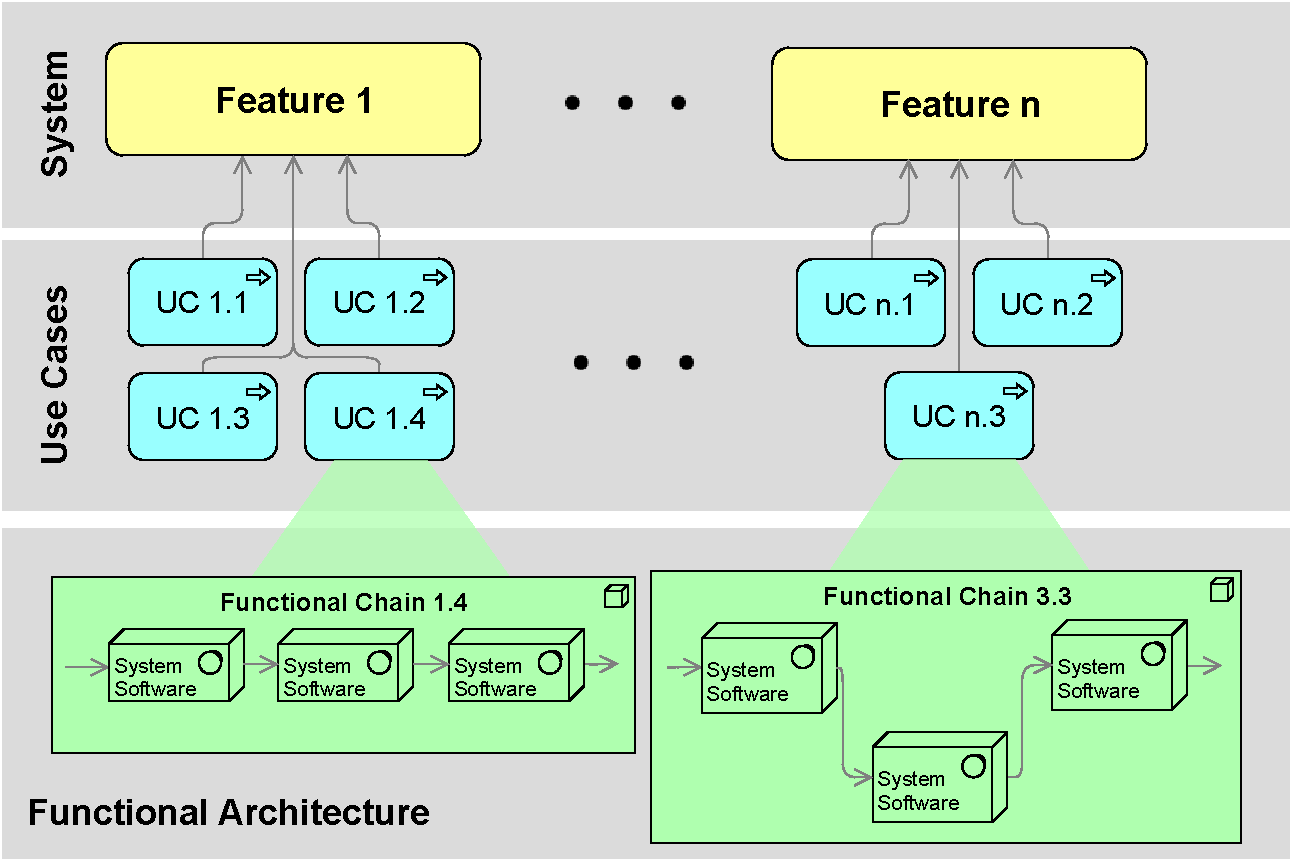
\includegraphics[width=\linewidth]{SchemaChaineFonctionnelle.pdf}
			\caption{Définition d'architecture fonctionnelle}
			\label{fig:funcArch}
		\end{figure}
	
		Il faut considérer les chaînes de tâches comme une implémentation d'une fonctionnalité système, qui va de son déclenchement jusqu'à sa terminaison. Cela correspond une majeure partie du temps à une chaîne de réaction allant d'une donnée d'entrée (détection d'un capteur par exemple) jusqu'à la conséquence (activation d'un actionneur), en passant par un algorithme de décision. Il s'agit donc d'un modèle classique de type Sense-Compute--Control où en pratique le Compute est implémenté par une Chaîne de tâches.
		Comme on l'a vu en début de ce Chapitre, il n'est pas tout à fait pertinent d'associer directement des niveaux de criticités au sens des standards logiciels de Sûreté de Fonctionnement (ASIL D à ASIL A et QM pour ISO 26262 en automobile typiquement), aux niveaux de criticités pour l'Agent de Surveillance et de Contrôle. Le seul lien qu'il est possible de déduire de la classification ASIL étant plutôt qu'il est improbable que les tâches de la chaîne critique soient de niveau QM. Les tâches de niveau d'ASIL élevé (ASIL D au maximum) feront certainement part de la chaîne de tâches critiques, mais il est difficile à partir d'un niveau d'ASIL plus faible d'en déduire le niveau d'importance d'une tâche. Ce critère d'importance étant crucial étant donné que les tâches non critiques du système pourront être mises en pause par l'agent de Surveillance et Contrôle.
		
	
		Si l'on revient au cas d'application automobile, les spécifications sont données par étapes. Dans un premier temps, il y a la spécification Système, qui liste la totalité des fonctionnalités (\emph{Features}) qui doivent être embarquées. Chaque Feature contient un certain nombre de Cas d'Utilisation (\emph{Use Cases}), qui se définissent par un scénario de fonctionnement et le comportement attendu de la fonctionnalité. Enfin, pour chaque Use Case, il est possible de représenter la Chaîne Fonctionnelle qui définit les blocs logiciels qui sont mobilisés pour réaliser ce cas d'utilisation. L'ensemble de ces chaînes constitue l'architecture fonctionnelle du système. Ces différentes couches de spécification système sont représentées dans la~\autoref{fig:funcArch}. %Si l'on va encore plus en détail dans la spécification, il y aurait ensuite l'allocation physique des blocs logiciels...
		

	
		On sent assez facilement que cette façon de modéliser le système est adaptée à notre approche pour identifier la méthode de sélection des tâches critiques, ainsi que quel type de spécification prendre en compte pour l'échéance d'exécution bout-en-bout, qui sont des données déjà existantes au niveau de l'architecture fonctionnelle. Une fois la chaîne fonctionnelle déterminée en fonction du système étudié, il est alors possible de descendre jusqu'à la spécification des tâches logicielles qui découlent cette architecture pour identifier les tâches critiques et non critiques.
		
\cmnt{
		\comment{A FAIRE}{Je pensais aborder dans cette section ce qui est repris ci-dessous en anglais, avec le lien entre les spécifications côté industrie et le choix de la chaîne de tâche. Mais au final ça fait beaucoup doublon avec ce que j'ai mis en début de chapitre, "Notion de criticité". Du coup je ne suis pas sûr de comment agencer tout ça. Et de voir comment j'inscris cette partie avec peut-être le fait de parler d'AUTOSAR / Adaptive AUTOSAR et ARINC 653...}
		% A critical task chain must describe the implementation of a system functionality from its triggering to its consequence. This would stick most of the time with a computing chain going from a sensor measure to an actuator command. First idea would be to stick with safety criticality levels (ASIL D to ASIL A and QM, for automotive applications), but we quickly notice that there is no direct link between this classification and critical tasks chains. A safety critical task is not necessarily defined from its timing constraints. The only possible conclusion here is that a critical task chain only includes non-QM tasks. 
		\smallbreak
		We propose here a definition based around high-level specifications as represented in figure~\ref{fig:funcArch}. The global system is defined as a set of features\footnote{Features: all the services the system must provide. e.g: Lane Support System (LSS) is a feature.}. Every feature gathers a set of functionalities that are translated into Use Cases\footnote{e.g: Lane Departure Warning \& Lane Keeping Assist are part of the use cases of LSS feature.}. A Use Case defines a feature behavior for a given context and inputs (and the consequent outputs). Finally, those are translated into functional chains representing different functions and their interactions needed for the realization of the Use Case. 


            
		If we combine this information with a severity classification in case of failure of the use cases, it is possible to define critical chains as functional chains with a high severity risk. This is one possible criterion allowing an easy separation between a critical functional chain and the others. It could be adapted during the design phase, depending on the functional chains allocated to the processor. 
		\smallbreak
		Such information allows to define the software components involved in the critical task chain. All the software components used to realize a critical functional chain form a critical task chain at an OS point of view. At this point, it is possible to define the task chain end-to-end deadline, following the severity temporal risk in case of failure. Such deadline should be at minimum the sum of individual tasks deadline, but could probably be higher, depending on the global system and the task chain function. Our objective is to guarantee such critical task chain end-to-end execution time on the multicore.
	}
		
\ifdefined\included
\else
\bibliographystyle{StyleThese}
\bibliography{these}
\end{document}
\fi

\ifdefined\included
\else
\documentclass[french, a4paper, 11pt, twoside, pdftex]{StyleThese}
\usepackage{iflang}
\usepackage{bibentry}



%\usepackage[sectionbib]{chapterbib}          % Cross-reference package (Natural BiB)
%\usepackage{natbib}                  % Put References at the end of each chapter
%\usepackage{bibunits}
% Do not put 'sectionbib' option here.
% Sectionbib option in 'natbib' will do.


\usepackage{fancyhdr}                    % Fancy Header and Footer

\usepackage[utf8]{inputenc}
\usepackage[T1]{fontenc}
\usepackage[french]{babel} %
\usepackage{lmodern} \normalfont %to load T1lmr.fd 
\DeclareFontShape{T1}{cmr}{b}{sc} { <-> ssub * cmr/bx/sc }{}
%\hyphenation{gar}

\usepackage{amsmath,amssymb}             % AMS Math
\usepackage{nicefrac}
\usepackage{siunitx}					%% Unites Math SI

\usepackage{blindtext}

\usepackage{datetime}

\usepackage{lipsum} 

\usepackage[inline]{enumitem}

\usepackage{hhline}
%\usepackage[left=1.5in,right=1.3in,top=1.1in,bottom=1.1in]{geometry}
\usepackage[left=1.5in,right=1.3in,top=1.1in,bottom=1.1in,includefoot,includehead,headheight=13.6pt]{geometry}

%%\renewcommand{\baselinestretch}{1.05}

%%%%%%%% Multi-figures avec sub-captions
\usepackage{caption}
\usepackage{subcaption}

% Table of contents for each chapter

\usepackage[nottoc, notlof, notlot]{tocbibind}
\usepackage[nohints]{minitoc}
\setcounter{minitocdepth}{2}
\mtcindent=15pt
% Use \minitoc where to put a table of contents

\usepackage{aecompl}

%% Package cosmetic meilleur layout du texte en jouant sur le spacing par caractères
\usepackage[activate={true,nocompatibility},final,tracking=true,kerning=true,factor=1100,stretch=10,shrink=10]{microtype}
\usepackage[absolute,overlay]{textpos} 
\setlength{\TPHorizModule}{\paperwidth}\setlength{\TPVertModule}{\paperheight}
\sloppy

%%%%%%%%%%% JOLIS TABLEAUX
\usepackage{tabularx}		%\usepackage{tabular}
\usepackage{longtable}
\usepackage{multirow}
\newcommand{\mc}{\multicolumn} 
\newcommand{\mr}[2]{\multirow{#1}{*}{#2}} 	\newcommand{\mrQ}{\multirow{-4}{*}}
\usepackage{booktabs}

\usepackage[usenames,dvipsnames]{xcolor} 

\makeatletter
\newcommand{\ccolor}[3][]{%
	\kern-\fboxsep
	\if\relax\detokenize{#1}\relax
	\expandafter\@firstoftwo
	\else
	\expandafter\@secondoftwo
	\fi
	{\colorbox{#2}}%
	{\colorbox[#1]{#2}}%
	{#3}\kern-\fboxsep
}
\makeatother

%%%%% Insertion graphiques format PGF
\usepackage{pgfplots}
\pgfplotsset{width=\linewidth, compat=1.16}%, compat=1.17}
\usepackage{adjustbox}          %%% PERMET DE LES RECADRER + FACILEMENT


%%%%%%%%%% Bullets de listes sans saut de ligne %%%%%%%%%%
\usepackage{xparse}

\ExplSyntaxOn%
\seq_new:N \l_local_enum_seq

\newcommand{\storethestuff}[1]{%
  \seq_set_from_clist:Nn \l_local_enum_seq {#1}%
}

\newcommand{\dotheenumstuff}{%
\int_zero:N \l_tmpa_int
\seq_map_inline:Nn \l_local_enum_seq {%
    \int_incr:N \l_tmpa_int% Increase the counter
    \item ##1
    % Check whether the list has reached the end -- if so, use '.' instead of ','
    %\int_compare:nNnTF 
    % { \l_tmpa_int } < {\seq_count:N \l_local_enum_seq} 
    % {,} {.}
  }
}
\ExplSyntaxOff

\NewDocumentCommand{\linebullets}{+m}{%
  \storethestuff{#1}%
  \begin{enumerate*}[label={\alph*)},font={\bfseries},itemjoin={{, }}]
    \dotheenumstuff%
  \end{enumerate*}
}

\newcommand{\cmnt}[1]{}  %%%%% AJOUT DE COMMENTAIRE MULTILIGNES


%%%%%%%%%% ECRITURE CARACTERES DANS UN CERCLE %%%%%%%%%%
%\def\circleTxt[#1]{\raisebox{.5pt}{\textcircled{\raisebox{-1pt}{#1}}}}
\newcommand{\ctxt}[1]{\raisebox{.5pt}{\textcircled{\raisebox{-1.2pt}{#1}}}}
% Glossary / list of abbreviations

\usepackage[intoc]{nomencl}
\IfLanguageName{english}{%
\renewcommand{\nomname}{Glossary}
}{ %
\renewcommand{\nomname}{Liste des Abréviations}
}

\makenomenclature

% My pdf code

\usepackage{ifpdf}

\ifpdf
  \usepackage[pdftex]{graphicx}
  \DeclareGraphicsExtensions{.pdf,PDF,.png,PNG,.jpg,JPG}
  \usepackage[pagebackref,hyperindex=true]{hyperref} %% use \autoref{} instead of Table~\ref{}.
  \usepackage{tikz}
  \usetikzlibrary{arrows,shapes,calc}
\else
  \usepackage{graphicx}
  \DeclareGraphicsExtensions{.ps,.eps}
  \usepackage[a4paper,dvipdfm,pagebackref,hyperindex=true]{hyperref}
\fi

\graphicspath{{.}{schemas/}{graphiques/}{tables/}}

%% nicer backref links. NOTE: The flag ThesisInEnglish is used to define the
% language in the back references. Read more about it in These.tex

\IfLanguageName{english}{
\renewcommand*{\backref}[1]{}
\renewcommand*{\backrefalt}[4]{%
\ifcase #1 %
(Not cited.)%
\or
(Cited in page~#2.)%
\else
(Cited in pages~#2.)%
\fi}
\renewcommand*{\backrefsep}{, }
\renewcommand*{\backreftwosep}{ and~}
\renewcommand*{\backreflastsep}{ and~}
}{
\renewcommand*{\backref}[1]{}
\renewcommand*{\backrefalt}[4]{%
\ifcase #1 %
(Non cité.)%
\or
(Cité en page~#2.)%
\else
(Cité en pages~#2.)%
\fi}
\renewcommand*{\backrefsep}{, }
\renewcommand*{\backreftwosep}{ et~}
\renewcommand*{\backreflastsep}{ et~}
}

% Links in pdf
\usepackage{color}
\definecolor{linkcol}{rgb}{0,0,0.4} 
\definecolor{citecol}{rgb}{0.5,0,0} 
\definecolor{linkcol}{rgb}{0,0,0} 
\definecolor{citecol}{rgb}{0,0,0}
% Change this to change the informations included in the pdf file

\hypersetup
{
bookmarksopen=true,
pdftitle="Prévention des fautes temporelles sur architectures multicœur pour les systèmes à criticité mixte",
pdfauthor="Daniel LOCHE", %auteur du document
pdfsubject="Thèse", %sujet du document
%pdftoolbar=false, %barre d'outils non visible
pdfmenubar=true, %barre de menu visible
pdfhighlight=/O, %effet d'un clic sur un lien hypertexte
colorlinks=true, %couleurs sur les liens hypertextes
pdfpagemode=UseNone, %aucun mode de page
%pdfpagelayout=DoublePage, %ouverture en simple page
pdffitwindow=true, %pages ouvertes entierement dans toute la fenetre
linkcolor=linkcol, %couleur des liens hypertextes internes
citecolor=citecol, %couleur des liens pour les citations
urlcolor=linkcol %couleur des liens pour les url
}

% definitions.
% -------------------

\setcounter{secnumdepth}{3}
\setcounter{tocdepth}{2}

% Some useful commands and shortcut for maths:  partial derivative and stuff

\newcommand{\pd}[2]{\frac{\partial #1}{\partial #2}}
\def\abs{\operatorname{abs}}
\def\argmax{\operatornamewithlimits{arg\,max}}
\def\argmin{\operatornamewithlimits{arg\,min}}
\def\diag{\operatorname{Diag}}
\newcommand{\eqRef}[1]{(\ref{#1})}
\newcommand{\nline}{\smallbreak\noindent}

\usepackage{rotating}                    % Sideways of figures & tables

% \usepackage{txfonts}                     % Public Times New Roman text & math font
  
%%% Fancy Header %%%%%%%%%%%%%%%%%%%%%%%%%%%%%%%%%%%%%%%%%%%%%%%%%%%%%%%%%%%%%%%%%%
% Fancy Header Style Options

\pagestyle{fancy}                       % Sets fancy header and footer
\fancyfoot{}                            % Delete current footer settings

%\renewcommand{\chaptermark}[1]{         % Lower Case Chapter marker style
%  \markboth{\chaptername\ \thechapter.\ #1}}{}} %

%\renewcommand{\sectionmark}[1]{         % Lower case Section marker style
%  \markright{\thesection.\ #1}}         %

\fancyhead[LE,RO]{\bfseries\thepage}    % Page number (boldface) in left on even
% pages and right on odd pages
\fancyhead[RE]{\bfseries\nouppercase{\leftmark}}      % Chapter in the right on even pages
\fancyhead[LO]{\bfseries\nouppercase{\rightmark}}     % Section in the left on odd pages

\let\headruleORIG\headrule
\renewcommand{\headrule}{\color{black} \headruleORIG}
\renewcommand{\headrulewidth}{1.0pt}
\usepackage{colortbl}
\arrayrulecolor{black}

\fancypagestyle{plain}{
  \fancyhead{}
  \fancyfoot{}
  \renewcommand{\headrulewidth}{0pt} %%%%%%%%%%%%%%%%%%%%%%%%%%%%%%%%%%%%%%%%%%%%%%%%%%%%%%%%%%%%%%%%%%%%%%%%%%%%%%%%%%%%%
}

%\usepackage{MyAlgorithm}
%\usepackage[noend]{MyAlgorithmic}
%\usepackage[ED=EDSYS-SystEmb, Ets=INP]{tlsflyleaf}

%%% Clear Header %%%%%%%%%%%%%%%%%%%%%%%%%%%%%%%%%%%%%%%%%%%%%%%%%%%%%%%%%%%%%%%%%%
% Clear Header Style on the Last Empty Odd pages
\makeatletter

\def\cleardoublepage{\clearpage\if@twoside \ifodd\c@page\else%
  \hbox{}%
  \thispagestyle{empty}%              % Empty header styles
  \newpage%
  \if@twocolumn\hbox{}\newpage\fi\fi\fi}

\makeatother
 
%%%%%%%%%%%%%%%%%%%%%%%%%%%%%%%%%%%%%%%%%%%%%%%%%%%%%%%%%%%%%%%%%%%%%%%%%%%%%%% 
% Prints your review date and 'Draft Version' (From Josullvn, CS, CMU)
\newcommand{\reviewtimetoday}[2]{\special{!userdict begin
    /bop-hook{gsave 20 710 translate 45 rotate 0.8 setgray
      /Times-Roman findfont 12 scalefont setfont 0 0   moveto (#1) show
      0 -12 moveto (#2) show grestore}def end}}
% You can turn on or off this option.
% \reviewtimetoday{\today}{Draft Version}
%%%%%%%%%%%%%%%%%%%%%%%%%%%%%%%%%%%%%%%%%%%%%%%%%%%%%%%%%%%%%%%%%%%%%%%%%%%%%%% 

\newenvironment{maxime}[1]
{
	\def\Arg{#1}
\vspace*{0cm}
\hfill
\begin{minipage}{0.6\textwidth}%
%\rule[0.5ex]{\textwidth}{0.1mm}\\%
\hrulefill $\:$ \\%$\:$ {\bf #1}\\
%\vspace*{-0.25cm}
\it 
}%
{%
	
\hrulefill $\:$ {\bf \Arg}
\vspace*{0.5cm}%
\end{minipage}
}

\let\minitocORIG\minitoc
\renewcommand{\minitoc}{\minitocORIG \vspace{1.5em}}

%\usepackage{slashbox}

\newenvironment{bulletList}%
{ \begin{list}%
	{$\bullet$}%
	{\setlength{\labelwidth}{25pt}%
	 \setlength{\leftmargin}{30pt}%
	 \setlength{\itemsep}{\parsep}}}%
{ \end{list} }


%%%%%%% Outils pour \comment \alert \add %%%%%
\usepackage{easyReview}
\usepackage{soulutf8} % for accented letters

\let\newalert\alert
\renewcommand{\alert}[1]{\textit{\newalert{#1}}}

%\usepackage[commandnameprefix=ifneeded]{changes} %% \chhighlight and \chcomment to avoid collision with easyReview
\renewcommand{\epsilon}{\varepsilon}

% centered page environment

\newenvironment{vcenterpage}
{\newpage\vspace*{\fill}\thispagestyle{empty}\renewcommand{\headrulewidth}{0pt}}
{\vspace*{\fill}}

\usepackage{tablefootnote}

%%%%%% MISE EN FORME CADRES DEFINITIONS/THEOREMES/LEMES %%%%%%%%%%
\usepackage{amsthm}  % for theoremstyle

\theoremstyle{plain} 
\newtheorem{theorem}{Théorème}[section]
\newtheorem{corollary}{Corolaire}[theorem]

%\theoremstyle{lemma}
%\newtheorem{lemma}[theorem]{Lemme}


\theoremstyle{definition}
\newtheorem{definition}[theorem]{Définition}


\cmnt{
	\usepackage{ntheorem} %\usepackage{amsthm}  % for theoremstyle
	%\usepackage{mdframed}
	\usepackage[most]{tcolorbox}
	
	\theoremstyle{plain} 
	\theoremindent20pt
	\theoremheaderfont{\normalfont\bfseries\hspace{-\theoremindent}}
	\newtheorem{theorem}{Théorème}[section]
	\newtheorem{corollary}{Corolaire}[theorem]
	
	\theoremstyle{plain}
	\newtheorem{lemma}[theorem]{Lemme}
	
	
	\tcolorboxenvironment{theorem}{
		blanker,
		breakable,
		before skip=\topsep,
		after skip=\topsep,
		borderline west={1pt}{10pt}{double, shorten <=12pt}
	}
	
	\theorembodyfont{\normalfont}
	\theoremindent20pt
	\theoremheaderfont{\normalfont\bfseries\hspace{-\theoremindent}}
	\newtheorem{definition}[theorem]{Définition}
	
	
	\tcolorboxenvironment{definition}{
		blanker,
		breakable,
		before skip=\topsep,
		after skip=\topsep,
		borderline west={1pt}{10pt}{shorten <=12pt}
	}
}

\cmnt{ 
	\begin{theorem}
		Ceci est un Théorème.
	\end{theorem} 
	
	\begin{corollary}
		Ceci est un Corollaire.
	\end{corollary}
	
	\begin{definition}
		Ceci est une Définition.
	\end{definition}
	
	\begin{lemma}
		Ceci est un Lemme.
	\end{lemma}
}

\def\UrlBigBreaks{\do\/\do-\do:}
\usepackage{url}

\sloppy
\begin{document}
\setcounter{chapter}{3} %% Numéro du chapitre précédent ;)
\dominitoc
\faketableofcontents
\fi

\chapter{Protocole et démarche expérimentale} \label{chap:4_ProtocolExpe}
\minitoc

Jusqu'à présent, nous avons fait un état des lieux des enjeux liés à l'usage des calculateurs multicœurs dans le cadre d'applications à criticité mixte et en dégager une problématique. Après une revue des solutions existantes dans le domaine, nous avons présenté dans le \hyperref[chap:3_PrincipeArchi]{Chapitre précédent} nos hypothèses de travail ainsi que le modèle de notre mécanisme d'évitement de fautes temporelles basé sur la surveillance d'une Chaîne de tâches critiques. Nous allons maintenant aborder une méthodologie de mise en service et de calibration du mécanisme pour un cas d'application. Cela nous permettra d'identifier les fondamentaux qui serviront au cas d'étude du \hyperref[chap:5_ImplementationCase]{Chapitre suivant}.

Notre proposition méthodologique repose sur 3 grandes phases de conception. Nous développerons successivement les exigences liées à la phase de Conception et de caractérisation d'un cas de test. L'objectif de cette démarche expérimentale est de caractériser un jeu de tâches au regard de sa propension à provoquer des interférences, et sa sensibilités aux-dites interférences. 

Les étapes de calibration et d'ajustement du mécanisme ont pour but d'implémenter et de configurer le mécanisme de Surveillance et de Contrôle pour l'implémenter sur un système à criticité duale donné.

Enfin la phase de vérification consiste à mesurer les propriétés de notre mécanisme ainsi configuré, pour un système donné. Il s'agit de mesurer et d'analyser plusieurs métriques : la Qualité, la Fiabilité et la Performance, au regard de la capacité à respecter l'échéance bout-en-bout de la chaîne de tâche, à limiter le temps d'arrêt des tâches non critiques, et à éviter les faux-positifs.



\pagebreak

\section{Principe Général et Objectifs}
        L'objectif de ce Chapitre est de présenter notre protocole expérimental, pour répondre à deux objectifs~: 
        \begin{itemize}
        	\item Le premier de caractériser un système de tâches donné pour y définir une chaîne de tâches critiques ainsi que le profil temporel des différentes tâches. 
        	\item         Le second de calibration et de test de l'Agent de Surveillance et Contrôle.
        \end{itemize}
        Il est important de préciser que notre méthode se décompose en ces deux intérêts bien distincts. En effet, une première partie du protocole général qui a été mis en place dans le cadre de ces travaux s'inscrit dans la phase de conception et de spécification. Cette partie se destine à la mise en place d'un banc expérimental qui ne repose pas sur un système déjà existant. De fait, en l'absence d'un système réel avec ses  spécifications propres sur lesquelles se baser, il nous faut recréer un cas de test et donc en fixer les contraintes temporelles qui soient cohérentes avec les caractéristiques d'exécution du logiciel qui est utilisé. En conséquence, l'ajout d'étapes méthodologiques a été nécessaire pour donner des spécifications cohérentes à ce cas d'utilisation et connaître le comportement temporel de notre cas de test. 
        Une fois cet aspect traité, la seconde partie du protocole expérimental présente normalement les étapes nécessaires qui doivent s'intégrer au processus de développement et d'intégration préexistant pour y ajouter l'Agent de Surveillance et Contrôle, le calibrer et le tester.
        
        Ce chapitre se divise donc en deux sections qui correspondent aux processus susmentionnés. Ils permettront de définir en amont du développement et de l'intégration de la solution quelles sont les données dont nous disposons en entrée et quels sont les résultats attendus en sortie de chaque étape du processus. Dans un dernier temps, nous agrégerons tout cela pour constituer un protocole expérimental global qui sera celui-utilisé pour la suite dans le cadre de notre mise en application.
        
        \section{Protocole de conception d'un cas de test}
        
        Le protocole de conception d'un cas de test proposé se divise en 5 phases distinctes. L'objectif est d'extraite à partir d'un set de tâches logicielles donné un ensemble de tâches dont on connaît les profils d'exécution et la sensibilité aux interférences dans un cas artificiellement stressé au maximum. Ces informations permettent dans un second temps de sélectionner de façon pertinente les tâches qui constitueront un cas de test sur lequel implémenter le mécanisme de Surveillance et Contrôle. Le cas de test doit se composer d'une part d'un ensemble de tâches critiques d'une part et non critiques d'autre part. La caractérisation sert à identifier les tâches suivant des critères de stabilité et fiabilité (c.-à-d. variabilité d'exécution pour une même entrée), sensibilité aux interférences et part d'interférences générées par l'usage de ressources partagées.
        
        Ce processus est relativement important pour quantifier les effets de notre mécanisme. De fait, la problématique d'interférences inter-tâches à laquelle nous essayons de répondre est hautement dépendante du comportement des tâches, notamment par leur usage des ressources partagées. Pour cette raison, il est important d'avoir une bonne connaissance sur le logiciel sur lequel s'intègre un mécanisme censé limiter les conséquences de ces interférences. Cette démarche de caractérisation d'un jeu de tâches peut avoir son importance de la même manière pour un cas d'application industrielle déjà existant. De fait, particulièrement dans l'usage de logiciel en boite noire, il est essentiel d'avoir une bonne maîtrise de ses caractéristiques d'exécution. Particulièrement dans la connaissance du taux d'utilisation de chaque ressource et de leur influence sur les temps d'exécution. Cela offre des éléments de décision pour l'allocation physique et d'ordonnancement des tâches. De cette façon le risque d'erreur d'estimation ou d'effets de bords dans les choix d'intégration peuvent être anticipé, voire limité.
        
        Dans le cadre de nos expérimentations, l'objectif de ce protocole est de mesurer les métriques propres aux interférences inter-tâches~: l'empreinte mémoire des tâches, le nombre de lectures/écritures, le nombre d'appels système, la puissance de calcul utilisée (taux CPU) et bien entendu les temps d'exécution et la sensibilité à l'application d'un stress sur les ressources partagées. De cette analyse, on se focalisera donc sur l'exploitation des tâches qui sont relativement sensibles à ces interférences d'une part, et à celles qui ont une forte empreinte mémoire et/ou une grande demande en ressources de calcul d'autre part. Cette démarche permet aussi pour un jeu de tâches préexistant, qui n'a pas été conçu pour un contexte de tâches temps-réel tel qu'on l'envisage, d'éliminer celles qui ont un comportement non maîtrisé qui ne correspond pas à un minimum que l'on serait en droit d'espérer de logiciel embarqué (par exemple une tâche qui aurait des variations de temps d'exécution sans interférences d'un ou plusieurs ordres de grandeur entre les millisecondes et la seconde).
        
        \begin{table}[ht]
        	\centering
        	\caption{Protocole de caractérisation d'un jeu de tâches}
        	\label{tab:tableprotocoledesign}
        	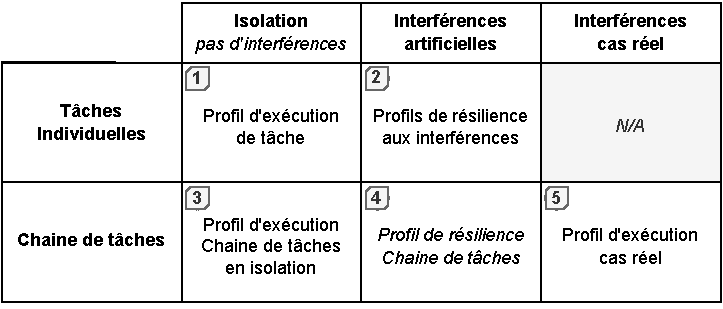
\includegraphics[width=0.8\linewidth]{tables/Table_Protocole_Design}
        \end{table}
             
        Pour arriver à cet objectif, nous allons travailler sur deux paramètres dans le cadre de ce protocole expérimental. D'une part nous allons faire varier la charge utile, qui est le logiciel monitoré pour en tirer ses caractéristiques, et d'autre part nous modifions les interférences -- le stress -- subi par la charge utile. Les différentes étapes du protocole sont agrégées dans le Tableau~\ref{tab:tableprotocoledesign}. La charge utile sera au choix soit une tâche spécifique, soit une chaîne de tâches telle que définie dans le chapitre précédent, tandis qu'elle sera soumise soit à~: \begin{enumerate}[label=\bfseries\alph*)] 
        	\item aucune interférence, donc en isolation,
        	\item des interférences imposées de façon artificielles par le biais de logiciels dédiés (comme \texttt{stress-ng} sous Linux) pour stresser au maximum le système,
        	\item les autres tâches du système, qui impliquent leurs propres interférences sur les ressources partagées.
        \end{enumerate}
    
        Suivant ces paramètres, le protocole de caractérisation se compose de cinq étapes, d'abord en caractérisant les tâches de façon individuelles, ensuite en caractérisant la chaîne de tâches critiques et enfin en vérifiant la pertinence des choix des tâches critiques et non critiques et de leurs paramètres, au regard de l'ordonnançabilité et de la présence d'interférences logicielles~: 
        \begin{itemize}
        	\item Profil d'exécution de chaque tâche
	        \begin{enumerate}[label=\large\ctxt{\arabic*}]
	        	\item tâches individuelles exécutées en isolation
	        	\item tâches individuelles exécutées avec stress imposé
	        \end{enumerate}
        	\item Profil d'exécution de la chaîne de tâches critiques
        	\begin{enumerate}[resume*]
        		\item chaîne de tâches en condition d'exécution en isolation
        		\item chaîne de tâches exécutée avec le stress artificiel
        	\end{enumerate}
        	\item Set de tâche complet
        	\begin{enumerate}[resume*]
        		\item chaîne de tâches \& tâches non-critiques qui constituent le cas de test 
        	\end{enumerate}
        \end{itemize}
    

	\subsection{Profil des tâches}
		Cette phase est nécessaire de façon à déterminer le profil d'exécution des tâches qui sont à notre disposition pour former un cas de test. Bien entendu, dans l'éventualité où l'on disposerait d'ores et déjà d'un jeu de tâches accompagné de leurs spécifications, il n'est pas nécessaire de réaliser ces étapes de profilage des tâches dans l'objectif d'y réaliser une sélection de tâches critiques et non-critiques pour constituer notre cas de test. Il est possible de passer directement à l'étape~\ctxt{3} pour caractériser la chaîne de tâches critiques au regard du système et vérifier la pertinence d'implémenter un mécanisme de surveillance et contrôle selon les variations de temps de réponse sur les tâches critiques. 
		
		Ceci étant dit, ces étapes peuvent tout de même être intéressantes dans un cas industriel où le jeu de tâches est déjà déterminé et spécifié en avance. Comme mentionné plus haut, cela peut apporter une connaissance plus détaillée des tâches et donc aider dans l'anticipation de risques d'interférences et dans le choix de l'allocation des tâches pour le prévenir.
		
		L'objectif de la phase de profilage est donc d'avoir les connaissances suffisantes sur les tâches en termes de temps d'exécution à la fois en cas optimal (aucune interférence) et au cas où la tâche subit un stress sur l'utilisation de ressources partagées. À cet effet, on peut mesurer des éléments subsidiaires tels que l'espace mémoire occupé, le nombre d'appels systèmes et le profil de lecture/calcul/écriture des tâches pour une analyse plus fine. À l'issue de ces tests, on doit être capable de spécifier quelles seront les tâches sélectionnées pour constituer le cas de test. Certaines tâches seront simplement éliminées à cause de caractéristiques compromettantes telles que des temps d'exécution trop variables ou différents des autres tâches pour cohabiter ou des problèmes de non-déterminisme. D'autres pourront être éligibles en tant que tâches critiques, de par une bonne fiabilité d'exécution. Enfin et surtout, il faudra inclure dans les tâches non-critiques au moins une part de tâches qui ont une forte influence sur l'utilisation des ressources partagées. Elles seront donc propices au déclenchement d'interférences sur les tâches critiques. Cette phase inclut donc les étapes \ctxt{1} et \ctxt{2}.
		
		\paragraph{\ctxt{1} - Tâches en Isolation}
			
			Cette première phase du processus consiste à exécuter une tâche individuelle sur la plateforme d'intégration en lui fournissant des données d'entrée de façon périodique. Sont mesurées les informations susmentionnées pour un nombre représentatif d'exécutions au regard de la variété possible des données d'entrée. 
			
			Dans le cas où l'on ne connaît pas l'ordre de grandeur des temps d'exécutions, il faudra prendre dans un premier temps une période d'exécution arbitraire relativement large (toutes les secondes par exemple). Il est possible ensuite de réduire ce temps pour que les tests soient plus rapides (toutes les 50ms pour une tâche qui prend autour de 20ms typiquement). Si le jeu de tâches dispose d'ores-et-déjà de spécifications sur les temps d'exécutions moyens, il est possible de choisir directement une valeur proche avec une marge de sûreté pour être sûr de la complétion systématique de la tâche.
			
			Ces mesures expérimentales doivent être reproduites pour chaque tâche, de façon à obtenir une table des caractéristiques de chaque tâche en isolation.
                    
    	\paragraph{\ctxt{2} - Tâches avec stress imposé artificiel}
    		
    		De la même façon que pour l'étape précédente, l'objectif est d'obtenir les mêmes informations de profilage des tâches dans une mise en situation où le matériel est soumis à un niveau de stress élevé sur l'utilisation des caches, des entrées/sorties et en usage CPU, tandis que la tâche testée est exécutée périodiquement pour une durée suffisante de façon à obtenir un échantillon représentatif. Cela est dépendant du système et de la tâche en question.
    		
    		Les étapes avec un stress imposé de façon artificielle sur le matériel par l'usage d'outils dédiés au stress. Plusieurs solutions sont possibles selon la plateforme de développement impliquée (matériel et logiciel). Pour mentionner quelques exemples, dans le cadre des travaux de~\cite{blin_maximizing_2016} des tâches dédiées ont été codées en assembleur pour effectuer des cycles d'accès mémoire sur une plateforme multicœur SABRE Lite. Sur des systèmes basés sur UNIX, il existe des outils comme \texttt{stress-ng}~\cite{king_stress-ng_2019} qui offrent toute une librairie d'utilitaires pour stresser des éléments spécifiques du processeur. Des travaux comme ceux de \cite{girbal_metrics_2018} proposent aussi un environnement de mesure des métriques d'exécution pour l'analyse de systèmes temps-réel sur multicœur.  
%%%% Je n'ai pas trouvé ECRTS 2021 (2020 ?) de Daniel Garcia Perez suggéré par ici...
	    	À l'issue de ces deux étapes de caractérisation, on dispose d'une matrice des caractéristiques du jeu de tâches qui inclut pour chaque tâche ses caractéristiques de temps de réponse en isolation et avec interférences sur les ressources partagées (i.e. stressée) et les compteurs pertinents (appels systèmes, préemptions...), tel qu'illustré dans le~\autoref{tab:tasksCaracs}. On y trouve les temps d'exécution minimum, médian, moyen et maximum, le nombre d'appels système, et éventuellement d'autres métriques propres à l'environnement d'exécution si elles sont pertinentes (nombre d'appels à un composant spécifique du firmware par exemple). 
	    	    	
	    	À partir de ces données, on peut alors identifier~:
	    	\begin{enumerate}
	    		\item Les tâches qui ne sont pas adaptées à nos besoins pour un cas de test. Soit parce que leurs temps d'exécution ne sont pas à la bonne échelle, c'est-à-dire avec des écarts d'ordre de grandeur trop importants. Par exemple des tâches trop macroscopiques qui prennent plusieurs secondes de calcul alors que le reste du système de tâche est composé de micro-tâches monofonctionnelles qui s'exécutent en quelques dizaines de millisecondes. Soit parce qu'elles ont été codées d'une manière qui ne semble pas acceptable, par exemple avec une surutilisation des appels système, qui provoquent des ralentissements indésirables trop dépendants du système d'exploitation.
	    		\item Les tâches qui sont appropriées pour servir de tâches non critiques qui vont provoquer des interférences. Ces dernières peuvent avoir des variations de temps d'exécution non négligeables et utiliser des ressources partagées.
	    		\item Enfin, les tâches qui peuvent servir en tant que tâches critiques, qui représentent alors a minima des tâches temps-réel souple avec peu, voire pas d'appels système et un fonctionnement maîtrisé en isolation (variations de temps d'exécution raisonnables), et potentiellement sensibles à des interférences, donc avec une variation non négligeable du temps d'exécution médian entre les 2 conditions de test.
	    	\end{enumerate}
	    		
	    	\begin{table}[h]
				\centering
				\caption{Template type des données de caractérisation des tâches}
				\label{tab:tasksCaracs}
				\begin{tabular}{@{}c cc ccc c ccc@{}}
					\toprule
					\mr{2}{Tâche}& \mr{2}{Appels Sys.} & \mr{2}{Autres appels} & \mc{3}{c}{en isolation} & \phantom{} & \mc{3}{c}{stressé} \\
					\cmidrule{4-6} \cmidrule{8-10}
					& & & $ t_{min} $ & $ t_{max} $ & $ t_{med} $ &\phantom{} &  $ t_{min} $ & $ t_{max} $ & $ t_{med} $  \\
					\midrule
					$\tau_1$ & -- & -- & -- & -- & -- &  & -- & -- & -- \\
					... 	 & -- & -- & -- & -- & -- &  & -- & -- & -- \\
					$\tau_n$ & -- & -- & -- & -- & -- &  & -- & -- & -- \\
					\bottomrule
				\end{tabular}
			\end{table} 
    		
    		À l'issue de cette sélection, on a donc à disposition un jeu de tâches, qui va être constitué d'une liste de \textbf{tâches non critiques} avec une période d'exécution pour chacune d'entre elle, et une liste de \textbf{tâches critiques} qui constituent la chaîne de tâches, qui doit donc inclure toutes les données relatives à la chaîne de tâches : période d'exécution de chaque tâche, mais aussi contraintes de précédence et échéance de temps de réponse bout-en-bout.
    		
    		Il s'avère que cette dernière donnée va être hautement dépendante des spécifications système dans le cadre d'un cas applicatif réel. 
    		
    		Dans une situation purement expérimentale où il nous faut constituer nous même le cas de test, cette donnée de temps de réponse bout-en-bout doit être fixée arbitrairement. Par conséquent, il va falloir là encore proposer une façon de fixer cette contrainte, ou au moins en définir un ordre de grandeur qui pourra être ajusté selon la difficulté que l'on souhaite imposer au test. Plus cette échéance est courte, plus il sera difficile de la garantir au regard des pires temps d'exécution des tâches et des risques d'allongement d'exécution inhérents notamment aux interférences
    		
                    
    \subsection{Profil du cas de test et Chaîne de tâches}
    
L'objectif de cette seconde phase de caractérisation consiste justement à caractériser plus globalement les tâches sélectionnées, notamment par la vérification de l'ordonnançabilité et de la contrainte de temps de réponse bout-en-bout de la chaîne. Il s'agit des étapes \ctxt{3}, \ctxt{4} et \ctxt{5} du protocole.

		\paragraph{\ctxt{3} - Chaîne de tâches critiques en isolation}
		Il est important de tester l'exécution de la chaîne de tâches en isolation, c'est-à-dire sans aucune interférence provenant des autres tâches qui doivent être intégrées. Cette étape permet de vérifier l'absence d'effets de bord entre la situation où les tâches étaient testées individuellement et le cas où la chaîne de tâches est exécutée sans aucune autre tâche non critique, donc en isolation. Le mode que l'on souhaite caractériser ici correspond, dans le cadre de l'utilisation du mécanisme de surveillance et de contrôle, au mode dégradé de fonctionnement. C'est-à-dire le mode d'exécution de la chaîne de tâches avec réduction des interférences par mise en pause des tâches non critiques. Cette caractérisation permet de définir le temps de réponse bout-en-bout que l'on sera capable de garantir en toute circonstance grâce à un passage en mode dégradé. En exécutant directement les tâches critiques en isolation, on peut connaître le profil de temps de réponse de la chaîne de tâches~: temps de réponse moyen et pire temps de réponse bout-en-bout. À partir de cette information, il devient possible de fixer dans notre spécification l'échéance de temps de réponse maximale permise pour la chaîne. Plus cette échéance sera proche du temps de réponse en isolation, plus cela implique que cette échéance est stricte dans le sens où elle est plus courte et donc difficile à tenir en cas de perturbations.
			
		Dans le cadre de nos expérimentations, nous fixons à cette étape deux éléments pour avancer dans les tests. Le premier sur la cohérence de la chaîne de tâches. Les tâches impliquées ici ayant un certain niveau de criticité, il semble pertinent de partir du principe qu'en l'absence de perturbations significatives l'écart entre le temps d'exécution minimal et maximal constatés pour la chaîne de tâches doivent être relativement restreints. Par conséquent, il faudra réviser le choix des tâches sélectionnées pour la chaîne dans le cas où l'on observe un écart trop significatif entre $ WCRT_{max} $ et $ WCRT_{min} $. Typiquement, si cet écart est supérieur à la moitié du temps de réponse médian observé. Ce qu'on l'on peut formaliser comme~: si $ WCRT_{max} - WCRT_{min} \leq 0.5*WCRT_{median} $ en isolation, alors la chaîne est suffisamment cohérente dans son comportement nominal. 
		Si cette conclusion est remplie, alors le second élément sera l'échéance de temps de réponse de référence que l'on pourra se fixer comme spécification, qui sera $D_C = 2*WCRT_{median}$. Il s'agit d'un choix réaliste qui peut être revu en fonction d'un contexte de système critique spécifique. Cela implique d'abord qu'en isolation, par définition on est garanti que la chaîne de tâches critiques est ordonnançable et ne peut pas dépasser son échéance et ensuite que l'on pourra ajuster cette échéance pour tester la fiabilité du mécanisme de Surveillance et Contrôle, en ayant cette valeur de référence comme base pour tester une spécification plus contraignante et donc difficile à respecter en cas d'interférences avec une échéance plus courte ou inversement .

		\paragraph{\ctxt{4} - Chaîne de tâches sous stress imposé}~\label{sec:pertinenceMecanisme}
		Il est possible de tirer parti des tâches de stress qui ont pu être utilisées pour la caractérisation individuelle de l'étape \ctxt{2} pour caractériser de la même façon la chaîne de tâches critiques qui a été sélectionnée. L'objectif est de s'assurer de la pertinence d'implémenter le mécanisme de Surveillance et Contrôle dans le cas d'étude que nous sommes en train de construire, en vérifiant que la chaîne de tâches peut effectivement être sujette à des interférences qui mènent à un dépassement d'échéance. 
		Le test consiste logiquement à exécuter la chaîne de tâches critiques sélectionnée avec les paramètres de l'étape précédente, conjointement aux tâches dédiées à la mise en stress du processeur sur les ressources partagées. En toute logique, on doit constater des dépassements de l'échéance de manière significative. Si aucune variation n'est constatée comparé au cas où la chaîne est isolée, alors les tâches sélectionnées ne sont pas sujettes aux interférences et donc il ne sera pas utile d'y adjoindre de mécanisme de contrôle. La chaîne choisie n'est a priori pas pertinente pour un cas de test.

		\paragraph{\ctxt{5} - Système complet dont chaîne de tâches critiques}
		Dans le cadre de mise en application de systèmes temps-réel à criticité mixte, il est nécessaire de passer par une phase de vérification d'ordonnançabilité. Cette phase est déjà partie intégrante des processus de développement industriels et propose de nombreux outils d'analyse tels que cela a été décrit dans le~\autoref{chap:2_StateofArt}. Nous n'avons pas approfondi en détail cette dimension de l'implémentation d'un set de tâches pour nous focaliser sur la proposition d'un mécanisme en lui-même en supposant que les vérifications d'usage d'ordonnançabilité sont validées. Il faut notamment noter que notre démarche véhicule l'espoir d'alléger les contraintes de garanties d'ordonnançabilité dans une certaine mesure. Notre positionnement étant que par la possibilité de passer en cas d'isolation qui permet de façon transitoire la garantie d'ordonnançabilité d'un sous-ensemble des tâches alors les preuves d'ordonnançabilité par estimation de pire temps d'exécution peuvent être allégées sur les tâches ciblées par le mécanisme.
		
		Par conséquent, dans cette étape, nous réalisons les vérifications d'ordonnançabilité du jeu de tâches sélectionnées sans rentrer dans des considérations trop approfondies tel que de la vérification formelle. De fait, on peut se permettre des dépassements d'échéances de façon marginale sur les tâches non-critiques (par définition) et sur les tâches critiques (avec la perspective de compenser cela via le mécanisme). Par conséquent, cette vérification peut se faire avec un niveau d'exigence et de certitude du résultat moins strict. Une possibilité consiste à vérifier d'abord de façon grossière via un calcul de taux d'occupation CPU moyen qui peut être ajusté avec la période d'exécution des tâches suivant la formule~:	$ \sum{\nicefrac{C_i}{T_i}} \leq 1 $ pour toutes les tâches allouées au même cœur pour un ordonnancement partitionné. Dans le cadre d'un ordonnancement global sur un processeur à N cœurs, on a aussi $ \sum{\nicefrac{C_i}{T_i}} \leq N $ (c.-à-d. avec possibilité de migration des tâches entre les cœurs). Et dans un second temps par une vérification expérimentale avec le cas de test complet tel que défini précédemment pour constater l'absence de dépassement d'échéances sauf éventuellement de façon marginale. Il existe des méthodes analytiques plus précises pour déterminer l'ordonnançabilité d'un set de tâches sur un calculateur multicœur. On pourra notamment mentionner \cite{melani_schedulability_2016} qui semble fort approprié dans le cadre de notre étude orientée sur des chaînes de tâches, ou encore plus généralement \cite{chen_efficient_2014} ou \cite{han_multicore_2018} pour des ordonnancements partitionnés. Si nous n'utilisons pas de telles méthodes, c'est avant tout parce qu'elles sont plus coûteuses en temps et complexité de mise en place. Elles peuvent nécessiter aussi des connaissances plus fines pour modéliser le système. Cela peut être parfaitement approprié, mais pas nécessaire dans notre cadre, d'autant plus pour un contexte industriel pour lequel des estimations approximatives sont souvent suffisantes.
			
		Dans un second temps la vérification est faite expérimentalement en surveillant l'exécution correcte des tâches selon les périodes fixées dans une mise en situation réelle la plus représentative possible.
		La question des conditions expérimentales est très riche et pourrait constituer un sujet de recherche en lui-même. Il est notamment question de définir la durée ainsi que la richesse des conditions de tests (représentativité des données d'entrée du test). En effet, dans l'idéal, il faut s'assurer que les durées d'expérimentation ainsi que la diversité des conditions de tests permettent une couverture suffisamment exhaustive pour couvrir tous les cas de fonctionnement du logiciel, même les plus spécifiques. 
		Dans le cas où l'on a à disposition les codes sources, cela peut être facilité par modélisation et étude analytique de façon à générer un modèle de test qui couvre tous les cas. Mais cela n'est plus possible à partir du moment où au moins une part du logiciel est en boite noire ou bien tout simplement si le logiciel a un niveau de complexité qui rend impossible de couvrir de façon exhaustive toute la combinatoire des possibilités d'exécution. Dans ce cas présent, nous sommes tenus à faire un choix d'un échantillon de test, classiquement de façon aléatoire. De même pour la durée de test, il faut \textit{a minima} considérer une durée qui permette à la fois d'avoir un régime de fonctionnement stable sur les mesures et une durée suffisante pour avoir un nombre de mesures qui limite statistiquement les marges d'erreur.
		Nous faisons donc le choix de données d'entrée aléatoire pour les tâches, avec une durée arbitraire de l'ordre de la minute qui nous a paru suffisant pour constater une stabilité des mesures. Il serait bien entendu possible d'affiner et perfectionner ces choix, mais ils présentent d'ores-et-déjà une base sur laquelle on pourra discuter et obtenir des premiers résultats.
		
		%%\comment{Choix du temps d'expérimentation et jeu de données d'entrée}{J'ai un peu éludé sur la question de combien de temps doivent durer les expérimentations et sur les éventuelles données d'entrée à utiliser qui se doivent représentatives et espérer couvrir les pires cas... C'est un "gros" morceaux en termes de temps que ça aurait demandé pour être fait de façon totalement exhaustive (la thèse de Mohammed est totalement dédiée à ça si je ne m'abuse) donc j'ai peur qu'en mettant le doigt dedans je complique trop les choses sans y apporter de réponse satisfaisante.}
		
		Cette étape permet aussi d'ores-et-déjà de constater le comportement de la chaîne de tâches critiques dans le cas nominal en l'absence de mécanisme pour contrôler d'éventuels augmentations indésirables de son temps de réponse. Il faut comparer ces temps de réponse avec les résultats obtenus à l'étape \ctxt{3}, qui correspond au cas de la chaîne est en isolation. Cela permet de quantifier l'influence spécifique à notre cas d'étude des interférences sur les tâches critiques et d'étudier la pertinence du choix d'échéance bout-en-bout qui a été fait à cette même étape. De fait, selon les temps de réponse constatés en fonctionnement normal sans mécanisme, sachant que la vérification de l'influence d'interférences a été effectuée à l'étape précédente, il est alors possible de voir si les tâches non-critique choisies ont effectivement, elles aussi, un effet significatif sur l'usage des ressources partagées. Si la chaîne de tâches critiques conserve un profil d'exécution similaire au cas en isolation, on est en mesure de dire que les tâches non-critiques choisies ne sont pas suffisantes pour avoir une influence sur les ressources partagées.
		
		Après avoir validé la définition des tâches critiques à l'étape précédente, on valide dans cette étape finale la définition des tâches non-critiques et donc du cas de test dans son ensemble.
		
		
		En conclusion, ce protocole simple en 5 étapes permet à partir d'un jeu de tâches dont nous ne connaissons pas les caractéristiques de spécifier un jeu de tâches contenant d'une part une chaîne de tâches critiques et d'autre part des tâches non critiques, avec leurs périodes, échéances implicites et répartition sur les cœurs. Ces étapes permettent par la même occasion de s'assurer un choix pertinent de tâches où le problème de respect d'échéance se pose au regard de l'influence des interférences sur les tâches critiques qui provoquent des retards d'exécutions qui peuvent potentiellement provoquer une faute temporelle.
                	
                	
\section{Protocole d'Implémentation et Calibration}

		En disposant d'un cas d'étude avec ses spécifications habituelles d'intégration du logiciel sur un calculateur multicœur, il nous est possible d'appliquer ce protocole de façon à calibrer le Mécanisme de Surveillance et Contrôle afin de garantir le respect d'échéance d'une chaîne de tâches critiques spécifique. Ce qui était désigné comme le cas en isolation dans le protocole de spécification précédent correspond alors, dans le cas de l'usage du mécanisme de Surveillance et de Contrôle, au passage en mode dégradé qui désactive les tâches non critiques pour retirer les interférences.
		
		De la même façon que pour le protocole de Conception d'un Cas d'Étude, nous nous basons ici aussi sur la mise au test de la chaîne  dans 3 contextes différents : en mode dégradé, avec des interférences matérielles imposées de façon artificielle et enfin avec toutes les tâches non-critiques, en d'autres termes le système complet. Le protocole se divise en deux temps avec~: 
		\begin{enumerate}
			\item Dans un premier temps la configuration des paramètres du mécanisme de Surveillance et de Contrôle. Il est alors exécuté uniquement pour sa composante de Surveillance pour récupérer les métriques nécessaires propres au système (temps de passage en mode dégradé, caractérisation des rWCRT de la chaîne...). 
			\item 		Dans un second temps, la composante de Contrôle est aussi activée pour tester effectivement le mécanisme selon les paramètres configurés, en mesurer les différentes métriques d'efficacité, et potentiellement réitérer sur le réglage des paramètres pour obtenir le comportement désiré.
		\end{enumerate}
		En résumé, et comme indiqué dans la~\autoref{tab:tableprotocoleImplementation}, pour calibrer le mécanisme de Surveillance et Contrôle implémenté, il est nécessaire de passer par 5 étapes~:
		\begin{itemize}
			\item \textbf{Spécification des paramètres} -- la chaîne de tâches est exécutée uniquement avec les fonctionnalités de Surveillance
			\begin{enumerate}[label=\large\ctxt{\arabic*}]
				\item Système exécuté en mode dégradé -- uniquement la chaîne de tâches
				\item Système complet exécuté -- tâches non-critiques incluses
			\end{enumerate}
			\item \textbf{Validation et mesures de comportement} -- la chaîne est exécutée avec le mécanisme complet activé
			\begin{enumerate}[resume*]
				\item Chaîne de tâches en conditions d'exécution du mode dégradé
				\item Chaîne de tâches exécutée avec charge de stress artificiel			
				\item Système complet exécuté -- tâches non-critiques incluses et mécanisme actif
			\end{enumerate}
		\end{itemize}
		\cmnt{\tikz
			\node[draw, chamfered rectangle, minimum width=.8\baselineskip, minimum height=.6\baselineskip,
			chamfered rectangle corners={south east, north west}, chamfered rectangle
			xsep=.02\baselineskip, inner sep=0pt] {1};}
		
		
		\begin{table}[ht]
			\centering
			\caption{Protocole d'implémentation et calibration du mécanisme}
			\label{tab:tableprotocoleImplementation}
			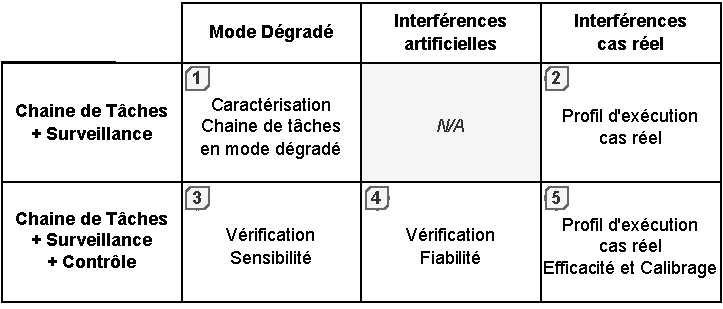
\includegraphics[width=0.8\linewidth]{tables/Table_Protocole_Implem}
		\end{table}
	
\pagebreak            
            
    \subsection{Spécification des paramètres de Contrôle}
    	L'étape \ctxt{1} de la calibration du mécanisme consiste à déterminer les grandeurs de paramétrage de ce dernier. Il est nécessaire de définir~: 
    	\begin{itemize}
    		\item $t_{sw}$ le temps de passage en mode dégradé ;
    		\item $T_{CCC}$ la période d'exécution du mécanisme de Surveillance et Contrôle ;
    		\item $rWCRT(\tau_{p})$ pour chaque tâche $\tau_p$ de la chaîne.
    	\end{itemize}
    
    	Le temps de passage en mode dégradé se calcule simplement de façon expérimentale, par mesures successives de déclenchement forcé du mode dégradé. Une valeur de borne maximale des mesures obtenue permet de garantir une estimation sûre de cette valeur. Dans les faits, cette valeur est relativement faible, voire négligeable. En effet, le passage en mode dégradé correspond à l'envoi d'un signal système qui met en pause les tâches non critiques. La durée de cette action dépend donc de deux éléments, d'abord du temps de réception du signal et ensuite du temps de mise en pause de la tâche. Ces derniers sont relativement faibles et la seule source de délai repose sur le temps de sauvegarde de contexte pour les tâches non critiques qui sont actuellement en cours d'exécution lors de la réception du signal.
    
    	\paragraph{\ctxt{1} -- Système exécuté en mode dégradé}
    	
    		Cette étape a pour objectif de déterminer deux des grandeurs susmentionnées. $T_{CCC}$ la période de vérification du mécanisme de contrôle. Et les différents $rWCRT(\tau_p)$ qui indiquent chacun la pire temps d'exécution restant garanti en mode dégradé pour la chaîne de tâche, selon le nombre de tâches restantes à exécuter pour la terminaison de la chaîne. 
    		
    		La chaîne de tâches est exécutée dans les mêmes conditions que le mode dégradé du système, avec le mécanisme qui est exécuté uniquement pour sa composante de Surveillance. Il convient donc de fixer en premier lieu le choix de $T_{CCC}$, qui est déterminé pour permettre au mécanisme implémenté de gérer la charge de réception des timestamps de terminaison des tâches critiques d'une part, et par le niveau de sensibilité à l'anticipation que l'on souhaite donner au mécanisme d'autre part. Il est ainsi hautement dépendant des spécifications de la partie critique du système. 
    		Pour donner une première valeur de période, nous nous focalisons sur la charge de réception. Il faut à chaque instant garantir qu'aucun timestamp ne soit perdu. Par conséquent, soit $L_{BUF}$ le nombre d'emplacements disponibles dans la mémoire tampon de réception des timestamps et $n$ le nombre de tâches critiques ayant pour périodes d'exécution $T_i, i \in [\![1,n]\!]$, alors la condition suffisante pour garantir le traitement de tous les timestamps est~:
    		\begin{equation}\label{eq:conditionsMemoireControle}
    			L_{BUF} \geq n  \quad \texttt{et} \quad T_{CCC} \leq \min{(T_i)}
    		\end{equation}
    		De cette façon, il est garanti qu'à chaque instant $t$, en pire cas le Core Control Component aura au maximum $n$ nouveaux timestamps à traiter, dans l'hypothèse --peu probable-- où toutes les tâches critiques se terminent en même temps. Une fois traités, ils sont ajoutés aux Traces d'Exécution actives gérée par la CCC pour le Contrôle.
    		De plus la récupération des timestamps doit être plus fréquente que l'occurrence de toute tâche critique, en particulier celle dont la période est la plus petite. En d'autres termes, le flux de traitement des timestamps par le mécanisme doit être supérieur au flux de terminaison des tâches critiques. 
    		Avec ces deux conditions, on a la garantie de ne perdre aucun timestamp envoyé. De fait, en considérant que chaque emplacement de la mémoire tampon correspond à une des tâches critiques, on a bien au moins 1 emplacement pour chaque tâche (première inéquation). Donc avec le mécanisme de contrôle qui s'exécute plus souvent que chacune des tâches critiques, on est sûr qu'il n'y aura pas plus d'un timestamp par tâche critique à gérer à chaque période de contrôle. On est donc sûr que la mémoire tampon n'aura pas de débordement et donc qu'aucun timestamp ne sera perdu. 
    		
    		Ces deux conditions de l'~\autoref{eq:conditionsMemoireControle} sont suffisantes, mais pas nécessaires. Cela fournit un premier couple de valeurs de période d'exécution et de taille de mémoire tampon simples et fonctionnels. Dans un cadre où la contrainte de mémoire disponible est très contraignante, il est probable que selon la chaîne de tâches étudiée, on puisse réduire taille de mémoire tampon, en calculant le nombre maximal de terminaison de tâches critiques possible durant une période de temps $T_{CCC}$.
    		Ou inversement, pour diminuer l'empreinte mémoire du mécanisme de surveillance et de contrôle, cette valeur de $T_{CCC}$ pourra être affinée en étape \ctxt{5}. Cela permet par la même occasion de jouer sur le niveau de sensibilité à l'anticipation du mécanisme, si nécessaire.
    		
    		Le mécanisme de surveillance est activé pour conserver les traces d'exécution de la chaîne de tâches $ET(j,t)$. 
    		Pour rappel, chaque trace d'exécution enregistre le timestamps de fin d'exécution de toutes les tâches de la chaîne selon le respect de la contrainte de précédence dans la chaîne. On reconstitue donc à partir de ces traces les temps d'exécution intermédiaires de la chaîne de tâche~: \\
    		pour chaque $p \in [\![1;n-1]\!], \quad ET(\,j\,,~t=succ^{\,p}(e_{1,j})~) = succ^{\,p}(e_{1,j}) - a_{1,j}$. \\
    		Comme on a pu le décrire en~\autoref{chap:3_PrincipeArchi}, les $e_{1,j}$ et $a_{1,j}$ correspondent respectivement aux dates de fin et d'activation du j\up{ème} job de la première tâche critique de la chaîne. Et $succ^{\,p}(e_{1,j})$ le timestamp de terminaison du p\up{ème} successeur du job d'entrée $\tau_{1,j}$ de la chaîne de tâches.
    		
    		En compilant tous les temps d'exécution intermédiaires obtenus, on peut en tirer des bornes maximales, qui correspondent alors aux différents $ rWCRT(\tau_p) $, on obtient~: \\
    		$\forall \ p \in [\![1\ ;\ n-1]\!], $, toutes les traces d'exécution obtenues :
    		
    		\begin{equation}
    			rWCRT(\tau_p) = \max_{j \in \mathbb{N^*}}\Big(~ET(\,j\,, succ^{\,p}(e_{1,j}) )~\Big) = \max_{j \in \mathbb{N^*}}\Big( succ^{\,p}(e_{1,j}) - a_{1,j} \Big) 
    		\end{equation} 
    	
    		Les $rWCRT(\tau_p)$ alimenteront donc la partie Contrôle du mécanisme pour son bon fonctionnement.
%           The task chain is then tested under a worst-case scenario. It is executed with the artificial system load, to stress as much as possible the task chain similarly to step \ctxt{2}. We get a baseline of the worst-case chain response time. This value is important because if the end-to-end deadline is always greater than the worst-case response time observed then the mechanism would be of no use (i.e. deadline never broken from temporal faults). This step gives a quantification of the task chain sensitivity to interferences and thus indicates the pertinence of using a Monitoring and Control Agent to manage them.
                    
                    
            \paragraph{\ctxt{2} -- Système complet avec Surveillance}
            
            Cette étape permet d'obtenir deux informations. La première essentielle est la valeur de $t_{SW}$, le temps de passage en mode dégradé. La seconde est la vérification de la pertinence d'utilisation du mécanisme de Surveillance et Contrôle. 
            
            De fait, en exécutant le système en condition normale de fonctionnement, adjoint au mécanisme de Surveillance sans activer le Core Control Component, il est possible de déclencher des transitions forcées aléatoires vers le mode dégradé, et d'en mesurer le temps de transition. Une borne supérieure aux valeurs mesurées permet de fixer $t_{SW}$.
            
            Par ailleurs, à l'image de ce qui a été fait dans le protocole de spécification d'un cas de test, en section~\ref{sec:pertinenceMecanisme}, on peut tirer profit de cette étape pour constater les potentielles fautes temporelles par dépassement de l'échéance bout-en-bout de la chaîne de tâches grâce à l'outillage de mesure permis par la Surveillance. Cette information de taux de dépassement d'échéance sur une mise en pratique expérimentale représentative offre une bonne base comparative pour les résultats ultérieurs qui seront obtenus après activation du mécanisme de contrôle.
            
            \smallbreak
            Suite à ces deux étapes, nous avons à disposition toutes les données et paramètres nécessaires à la mise en place du mécanisme complet de Surveillance et de Contrôle.
            L'objectif des étapes qui suivent dans le protocole est de quantifier l'efficacité du mécanisme. Cela est d'autant plus utile que les métriques proposées peuvent servir en retour pour ajuster les paramètres précédemment déterminés afin d'ajuster les propriétés et le comportement du mécanisme aux besoins du système. 
            
    \subsection{Calibration du Mécanisme de Contrôle}
    
    	\paragraph{\ctxt{3} -- Qualité du mécanisme}

    	Une première métrique d'analyse du mécanisme est la \textbf{qualité}. Cela consiste à identifier dans quelle mesure le mécanisme serait trop sensible, et donc déclencherait des passages en mode dégradé non nécessaires.
    	
    	Cette mesure est relativement complexe à obtenir de façon parfaite, dans le sens où cela nécessiterait d'identifier précisément pour chaque décision du mécanisme, si le passage en mode dégradé était nécessaire ou non. Hors, il n'est pas possible d'avoir un oracle parfait qui donnerait le résultat en cas de conservation du mode nominal à chaque instant où la décision a été prise. 
    	
    	Par conséquent, la mesure que nous allons considérer ici consiste à identifier les passages en mode dégradé dans un cas où l'on sait qu'il ne devrait en avoir aucun, c'est-à-dire en isolation. 
    	Un test que nous réalisons consiste donc à exécuter le système directement en mode dégradé, avec les tâches non critiques qui ne sont pas exécutées, mais le mécanisme complètement actif.
    	De cette façon, on mesure la qualité du mécanisme à partir de son comportement dans un cadre où \textit{a priori} il ne devrait pas déclencher de mode dégradé, par absence d'interférences. Tout passage en mode dégradé dans ces conditions sera alors \textit{de facto} un faux positif.
    	En dénombrant les passages en mode dégradé dans de telles conditions expérimentales, on a alors une première idée de la qualité du mécanisme. Plus le nombre de faux positifs sera élevé, moins la qualité sera bonne.
    	
    	Aussi, il existe des variables d'ajustements pour influer sur la qualité du mécanisme. Le principal facteur est sa période d'exécution $T_{ccc}$. De fait, plus le nombre de changements de modes est élevé, plus cela signifie que le mécanisme est sensible. Cela peut être alors dû à deux éléments : 
    	\begin{itemize}
    		\item Soit la période d'exécution du mécanisme de contrôle est trop grande, ce qui fait que la constante $W_{MAX}$ dans~\autoref{eq:safe_cond} de l'anticipation est trop prépondérante. Cela provoque une anticipation qui se base sur un point de contrôle suivant trop lointain. La vérification de l'absence de risque de dépassement prend en considération une période avant le prochain point de contrôle trop grande, ce qui augmente d'autant la potentialité d'un risque de dépassement. Pour obtenir une bonne anticipation du risque de viol de l'échéance la prise de décision devrait se baser en premier lieu sur les grandeurs dynamiques du système, qui évoluent au fil de l'exécution, donc $RT(t)$ et $rWCRT(t)$. En d'autres termes, plus la période de contrôle est grande, plus le risque de dépassement anticipé entre deux périodes est grand, et donc plus le mécanisme est sensible. Diminuer la période améliore la sensibilité, au coût d'une plus grande utilisation du CPU.
    		\item Soit les ordres de grandeur impliqués entre les temps d'exécution des tâches avec et sans perturbations sont trop proches au regard des autres grandeurs du système (période de surveillance notamment), ce qui rend la différenciation entre un cas à risque et un cas nominal bien trop subtil pour être discriminé par le mécanisme. Cela peut être dû aux estimations trop pessimistes qui ont été faites sur les pires temps de réponse restants, autrement, il est possible que l'échéance fixée soit simplement trop stricte et en conséquence trop proche des temps de réponse constatés lors d'un fonctionnement sans aucune interférence. Auquel cas ce genre de mécanisme n'est pas adapté et il faudra se contenter des méthodes plus classiques de contrôle statique au détriment de l'optimisation de la puissance de calcul.
    	\end{itemize}
    	Dans l'idéal, il faudrait qu'aucun déclenchement de mode dégradé ne soit constaté dans ce cadre-ci. Dans de telles conditions, cela indique potentiellement qu'une plus grande période d'exécution du mécanisme est possible, afin d'alléger son empreinte sur l'utilisation du processeur. Cela reste bien entendu conditionné à la capacité de réception de tous les timestamps bien entendu, selon la condition présentée en ~\autoref{eq:conditionsMemoireControle}.
    	
    	\paragraph{\ctxt{4} -- Fiabilité du Mécanisme}
        En exécutant la chaîne de tâches critique avec le Contrôle opérationnel dans un contexte où le processeur est le plus stressé possible en terme d'interférence, il est possible de mesurer la \textbf{fiabilité} du mécanisme.
        Dans un tel contexte pire cas, il est possible de vérifier si les paramètres de contrôle choisis sont corrects. Si tel est le cas, on ne devrait observer aucun dépassement d'échéance bout-en-bout lors de ces tests. 
        S'il advenait que l'échéance de temps de réponse bout-en-bout ne soit pas respectée un certain nombre de fois, alors il serait essentiel d'approfondir la question pour remonter aux raisons de ces fautes.
        
		Il peut y avoir deux explications à de tels dépassements. Il peut s'agir simplement d'une sous estimation des $rWCRT(\tau_p) $, qui a mené à un déclenchement du mode dégradé trop tardif.
        Cela doit pouvoir s'observer via la trace d'exécution de la chaîne de tâches qui a conduit au dépassement. On devrait observer un profil d'exécution dans les tranches hautes de temps de réponse habituellement observés pour la chaîne de tâches (et donc proche, mais inférieur aux valeurs de $rWCRT(\tau_p)$ paramétrées), mais pas suffisamment pour que le déclenchement du mode dégradé se soit fait assez tôt.
        
        En revanche si cela n'est pas constaté et qu'il y a dépassement d'échéance malgré le mécanisme de Contrôle semble qui s'être déclenché dans les temps, alors il est possible que ce soit dû à des facteurs non contrôlés par le mécanisme. Plus spécifiquement, il peut s'agir de retards d'exécution qui ne proviennent pas des interférences matérielles liées aux tâches non-critiques.
        Si ce cas est souligné ici, c'est parce qu'il est vraisemblable lorsque ce genre de mécanisme est utilisé dans un environnement complexe où tout ce qui se produit au niveau du système d'exploitation n'est pas parfaitement maîtrisé. Cela est particulièrement le cas avec l'usage de plus en plus fréquent de distributions Linux pour les systèmes embarqués. Plusieurs travaux tels que~\cite{allende_towards_2019} ou encore \cite{sivakumar_automotive_2020} et \cite{serra_architecture_2020} se sont intéressés aux conditions de mise en place d'un tel système pour du temps-réel, les difficultés que cela implique ainsi que ce que l'on peut attendre de Linux dans ces conditions. Cette étape de vérification de la fiabilité peut donc permettre de soulever des problèmes externes propres au matériel ou au logiciel sous-jacent, qui devront être résolus par ailleurs. Cela peut provenir de l'utilisation de drivers inadaptés, ou de l'exécution de code non stoppé avec les tâches non critiques (tâches système, typiquement). Dans un contexte industriel avec un OS dédié, cette seconde source ne devrait logiquement pas exister. 
                    
		\paragraph{\ctxt{5} -- Système complet avec mécanisme de contrôle}
		 Pour finir, la dernière étape du protocole de calibration et d'implémentation du mécanisme consiste simplement à exécuter la totalité du système en mode nominal, accompagné du mécanisme de surveillance et de contrôle. 
		 Cette dernière phase d'essai a, elle aussi, pour objectif d'apporter des métriques d'analyse de fonctionnement du mécanisme. Nous avons mesuré jusqu'à présent la fiabilité et la qualité de ce dernier. Il reste alors la \textbf{performance}, qui regarde dans quelle mesure nous réussissons à conserver l'exécution des tâches non critiques malgré l'ajout du mécanisme de contrôle.
		 En réalisant ce test dans les mêmes conditions que l'étape \ctxt{2} où la partie Contrôle était inactive, on peut donc comparer le temps d'exécution et le nombre de jobs réalisés pour chaque tâche non critique, au regard de la diminution du nombre de dépassements d'échéances. On devrait normalement constater un taux de dépassement de l'échéance qui devient nul en cas d'une fiabilité de 100\%.
		 Par la même occasion, on peut mesurer le temps d'exécution moyen du mécanisme de surveillance et contrôle en fonctionnement nominal, de façon à vérifier que son empreinte d'utilisation du CPU est non significative et n'empiète donc pas sur les performances globales, ce qui serait bien entendu contre-productif.
		 
		 Cette étape est enfin l'occasion de faire varier les paramètres de configuration du Contrôle en réitérant sur les 2 étapes précédentes, pour ajuster les performances mesurées du mécanisme aux besoins spécifiques de l'application si nécessaire. Ainsi il sera possible de modifier la période d'exécution du Contrôle soit  pour diminuer son utilisation du CPU dans le cas d'un taux d'utilisation considéré trop élevé, soit parce que l'on a constaté une sensibilité trop élevée, par un nombre de faux positifs trop grand.
		 Il est aussi possible d'accepter de façon exceptionnelle des dépassements de l'échéance bout-en-bout, dans un modèle où la chaîne serait à temps-réel souple typiquement ou si l'on veut garantir un niveau de Qualité de Service (\textit{QoS}) comme cela a pu être développé dans des études comme~\cite{lin_maximizing_2006}. Pour ce faire, on peut revoir les valeurs de $rWCRT(\tau_p)$ à la baisse. Cela revient à fixer les pires temps d'exécution restant garantis en mode dégradé à des valeurs plus optimistes. Par conséquent, la sensibilité du mécanisme sera allégée au détriment de dépassements d'échéance de façon occasionnelle malgré le passage en mode dégradé, typiquement quand le temps de réponse en mode dégradé sera situé juste au dessus des nouveaux seuils de $rWCRT(\tau_p)$ qui ont été abaissés. Cela donnera alors une fiabilité inférieure à 100\% de garantie de l'échéance, mais qui peut être ajustée expérimentalement pour rester à un taux d'occurrences maîtrisé. Il serait alors possible par calcul probabiliste de fixer une baisse de ces valeurs pour obtenir au niveau souhaité de taux de défaillance temporelle sur la chaîne de tâches critiques, typiquement.
		 
		 Ces ajustements des paramètres du mécanisme sont des possibilités offertes par ce dernier, hautement dépendantes de besoins spécifiques. Nous étudierons plus en détail l'influence de variation de ces valeurs dans la suite des travaux. Le protocole expérimental d'analyse du mécanisme étant clos ici.    	
                	
                	
\section{Protocole expérimental global}
    
    Pour la suite de nos travaux, comme l'on peut s'en douter nous avons dû mettre en œuvre les deux protocoles expérimentaux présentés ici. En premier lieu le protocole de spécification d'un cas de test mis en application sur une suite logicielle de benchmarking. Et ensuite le protocole d'implémentation du mécanisme de surveillance et de contrôle sur le cas de test précédemment spécifié. Par conséquent, nous présentons en conclusion de cette partie le tableau récapitulatif expérimental, dans le cas où ces 2 méthodes doivent être employées successivement.
    
    Il est à noter que les deux protocoles se recoupent en partie, dans les conditions expérimentales de test de la chaîne de tâches critiques. Il s'agit de la seconde ligne du~\autoref{tab:tableprotocoledesign} où la chaîne de tâches est caractérisée, qui propose les mêmes conditions expérimentales que la première ligne du~\autoref{tab:tableprotocoleImplementation}. La nuance à noter est que là où le protocole de Spécification propose une caractérisation de la chaîne de tâches \textit{en isolation}, dans le cadre de l'implémentation du mécanisme de contrôle, ces conditions de test doivent correspondre au cas exact dans lequel sera le système en mode dégradé. Il s'agit alors d'un cas où la chaîne de tâche est isolée d'interférences des tâches non critiques, mais cela implique aussi une configuration spécifique des tâches critiques, notamment sur leur allocation physique sur les cœurs du processeur. 
    En bref, tout cela pour exprimer que la caractérisation de la chaîne de tâche doit se faire dans les mêmes conditions que celles qui seront impliquées lors d'un passage en mode dégradé par le mécanisme de contrôle.
    
    \begin{table}[ht]
    	\centering
    	\caption{Protocole "Complet" de Spécification, Caractérisation et Analyse}
    	\label{tab:tableprotocoleComplet}
    	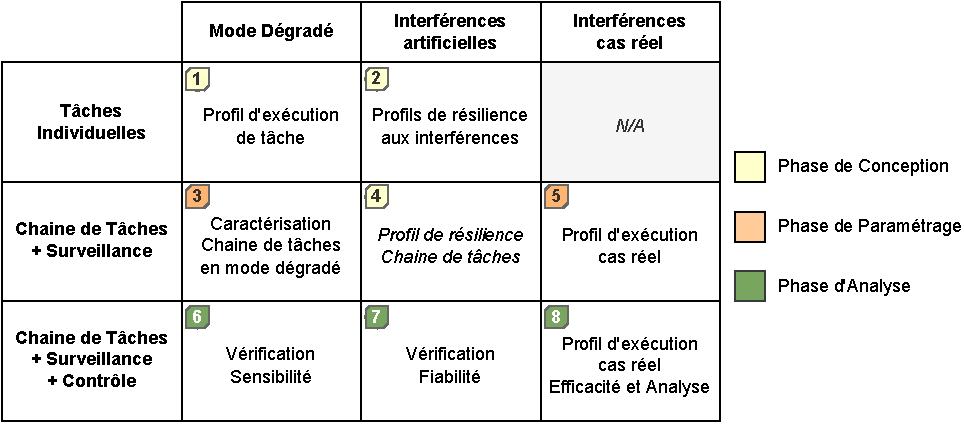
\includegraphics[width=\linewidth]{Table_Protocole_Complet}
    \end{table}

   	En bilan, nous avons donc le~\autoref{tab:tableprotocoleComplet} qui donne 3 Phases expérimentales : la Conception, le Paramétrage et l'Analyse. 
   	
   	Lors de la phase de Conception, sont testées successivement les tâches de façon individuelle pour en obtenir une caractérisation temporelle. Cela permet d'avoir une meilleure connaissance des temps d'exécutions des tâches et de leur propension à introduire et/ou recevoir des interférences sur l'utilisation de ressources partagées. Dans le cas où il ne s'agit pas d'un jeu de tâches déjà spécifié pour un système industriel, il s'agit aussi de constituer la sélection d'un jeu de tâches de test à partir de tâches provenant d'un benchmark ou autre. Cela permet de spécifier les tâches non critiques et les tâches critiques sous forme d'une chaîne de tâches. Dans cette éventualité, la phase de conception propose enfin la vérification des choix effectués notamment en termes de taux d'utilisation du processeur et de la présence manifeste d'interférences qui peuvent mener à des dépassements d'échéances.
   	
   	Vient ensuite la phase de Paramétrage, qui repose sur l'exécution de la chaîne de tâches critiques uniquement pour déterminer les paramètres du mécanisme de Surveillance et Contrôle.
   	
   	Pour finir, la phase d'Analyse intègre la chaîne de tâches avec l'ajout du mécanisme complet. Chaque test est soumis soit à aucune interférence matérielle spécifique (cas en mode dégradé), soit avec des interférences imposées de façon artificielle pour s'approcher d'un "pire cas" de charge, soit avec la charge réelle qui inclut les interférences inhérentes à toutes les tâches du système, notamment les tâches non critiques. De ces tests, on est en mesure de définir les propriétés du mécanisme de Surveillance et Contrôle selon des critères de Fiabilité, Qualité et Performance tel que présentés précédemment. 
   	

   	
\ifdefined\included
\else
\bibliographystyle{StyleThese}
\bibliography{these}
\end{document}
\fi


\ifdefined\included
\else
\documentclass[a4paper,11pt,twoside]{StyleThese}
\usepackage{iflang}
\usepackage{bibentry}



%\usepackage[sectionbib]{chapterbib}          % Cross-reference package (Natural BiB)
%\usepackage{natbib}                  % Put References at the end of each chapter
%\usepackage{bibunits}
% Do not put 'sectionbib' option here.
% Sectionbib option in 'natbib' will do.


\usepackage{fancyhdr}                    % Fancy Header and Footer

\usepackage[utf8]{inputenc}
\usepackage[T1]{fontenc}
\usepackage[french]{babel} %
\usepackage{lmodern} \normalfont %to load T1lmr.fd 
\DeclareFontShape{T1}{cmr}{b}{sc} { <-> ssub * cmr/bx/sc }{}
%\hyphenation{gar}

\usepackage{amsmath,amssymb}             % AMS Math
\usepackage{nicefrac}
\usepackage{siunitx}					%% Unites Math SI

\usepackage{blindtext}

\usepackage{datetime}

\usepackage{lipsum} 

\usepackage[inline]{enumitem}

\usepackage{hhline}
%\usepackage[left=1.5in,right=1.3in,top=1.1in,bottom=1.1in]{geometry}
\usepackage[left=1.5in,right=1.3in,top=1.1in,bottom=1.1in,includefoot,includehead,headheight=13.6pt]{geometry}

%%\renewcommand{\baselinestretch}{1.05}

%%%%%%%% Multi-figures avec sub-captions
\usepackage{caption}
\usepackage{subcaption}

% Table of contents for each chapter

\usepackage[nottoc, notlof, notlot]{tocbibind}
\usepackage[nohints]{minitoc}
\setcounter{minitocdepth}{2}
\mtcindent=15pt
% Use \minitoc where to put a table of contents

\usepackage{aecompl}

%% Package cosmetic meilleur layout du texte en jouant sur le spacing par caractères
\usepackage[activate={true,nocompatibility},final,tracking=true,kerning=true,factor=1100,stretch=10,shrink=10]{microtype}
\usepackage[absolute,overlay]{textpos} 
\setlength{\TPHorizModule}{\paperwidth}\setlength{\TPVertModule}{\paperheight}
\sloppy

%%%%%%%%%%% JOLIS TABLEAUX
\usepackage{tabularx}		%\usepackage{tabular}
\usepackage{longtable}
\usepackage{multirow}
\newcommand{\mc}{\multicolumn} 
\newcommand{\mr}[2]{\multirow{#1}{*}{#2}} 	\newcommand{\mrQ}{\multirow{-4}{*}}
\usepackage{booktabs}

\usepackage[usenames,dvipsnames]{xcolor} 

\makeatletter
\newcommand{\ccolor}[3][]{%
	\kern-\fboxsep
	\if\relax\detokenize{#1}\relax
	\expandafter\@firstoftwo
	\else
	\expandafter\@secondoftwo
	\fi
	{\colorbox{#2}}%
	{\colorbox[#1]{#2}}%
	{#3}\kern-\fboxsep
}
\makeatother

%%%%% Insertion graphiques format PGF
\usepackage{pgfplots}
\pgfplotsset{width=\linewidth, compat=1.16}%, compat=1.17}
\usepackage{adjustbox}          %%% PERMET DE LES RECADRER + FACILEMENT


%%%%%%%%%% Bullets de listes sans saut de ligne %%%%%%%%%%
\usepackage{xparse}

\ExplSyntaxOn%
\seq_new:N \l_local_enum_seq

\newcommand{\storethestuff}[1]{%
  \seq_set_from_clist:Nn \l_local_enum_seq {#1}%
}

\newcommand{\dotheenumstuff}{%
\int_zero:N \l_tmpa_int
\seq_map_inline:Nn \l_local_enum_seq {%
    \int_incr:N \l_tmpa_int% Increase the counter
    \item ##1
    % Check whether the list has reached the end -- if so, use '.' instead of ','
    %\int_compare:nNnTF 
    % { \l_tmpa_int } < {\seq_count:N \l_local_enum_seq} 
    % {,} {.}
  }
}
\ExplSyntaxOff

\NewDocumentCommand{\linebullets}{+m}{%
  \storethestuff{#1}%
  \begin{enumerate*}[label={\alph*)},font={\bfseries},itemjoin={{, }}]
    \dotheenumstuff%
  \end{enumerate*}
}

\newcommand{\cmnt}[1]{}  %%%%% AJOUT DE COMMENTAIRE MULTILIGNES


%%%%%%%%%% ECRITURE CARACTERES DANS UN CERCLE %%%%%%%%%%
%\def\circleTxt[#1]{\raisebox{.5pt}{\textcircled{\raisebox{-1pt}{#1}}}}
\newcommand{\ctxt}[1]{\raisebox{.5pt}{\textcircled{\raisebox{-1.2pt}{#1}}}}
% Glossary / list of abbreviations

\usepackage[intoc]{nomencl}
\IfLanguageName{english}{%
\renewcommand{\nomname}{Glossary}
}{ %
\renewcommand{\nomname}{Liste des Abréviations}
}

\makenomenclature

% My pdf code

\usepackage{ifpdf}

\ifpdf
  \usepackage[pdftex]{graphicx}
  \DeclareGraphicsExtensions{.pdf,PDF,.png,PNG,.jpg,JPG}
  \usepackage[pagebackref,hyperindex=true]{hyperref} %% use \autoref{} instead of Table~\ref{}.
  \usepackage{tikz}
  \usetikzlibrary{arrows,shapes,calc}
\else
  \usepackage{graphicx}
  \DeclareGraphicsExtensions{.ps,.eps}
  \usepackage[a4paper,dvipdfm,pagebackref,hyperindex=true]{hyperref}
\fi

\graphicspath{{.}{schemas/}{graphiques/}{tables/}}

%% nicer backref links. NOTE: The flag ThesisInEnglish is used to define the
% language in the back references. Read more about it in These.tex

\IfLanguageName{english}{
\renewcommand*{\backref}[1]{}
\renewcommand*{\backrefalt}[4]{%
\ifcase #1 %
(Not cited.)%
\or
(Cited in page~#2.)%
\else
(Cited in pages~#2.)%
\fi}
\renewcommand*{\backrefsep}{, }
\renewcommand*{\backreftwosep}{ and~}
\renewcommand*{\backreflastsep}{ and~}
}{
\renewcommand*{\backref}[1]{}
\renewcommand*{\backrefalt}[4]{%
\ifcase #1 %
(Non cité.)%
\or
(Cité en page~#2.)%
\else
(Cité en pages~#2.)%
\fi}
\renewcommand*{\backrefsep}{, }
\renewcommand*{\backreftwosep}{ et~}
\renewcommand*{\backreflastsep}{ et~}
}

% Links in pdf
\usepackage{color}
\definecolor{linkcol}{rgb}{0,0,0.4} 
\definecolor{citecol}{rgb}{0.5,0,0} 
\definecolor{linkcol}{rgb}{0,0,0} 
\definecolor{citecol}{rgb}{0,0,0}
% Change this to change the informations included in the pdf file

\hypersetup
{
bookmarksopen=true,
pdftitle="Prévention des fautes temporelles sur architectures multicœur pour les systèmes à criticité mixte",
pdfauthor="Daniel LOCHE", %auteur du document
pdfsubject="Thèse", %sujet du document
%pdftoolbar=false, %barre d'outils non visible
pdfmenubar=true, %barre de menu visible
pdfhighlight=/O, %effet d'un clic sur un lien hypertexte
colorlinks=true, %couleurs sur les liens hypertextes
pdfpagemode=UseNone, %aucun mode de page
%pdfpagelayout=DoublePage, %ouverture en simple page
pdffitwindow=true, %pages ouvertes entierement dans toute la fenetre
linkcolor=linkcol, %couleur des liens hypertextes internes
citecolor=citecol, %couleur des liens pour les citations
urlcolor=linkcol %couleur des liens pour les url
}

% definitions.
% -------------------

\setcounter{secnumdepth}{3}
\setcounter{tocdepth}{2}

% Some useful commands and shortcut for maths:  partial derivative and stuff

\newcommand{\pd}[2]{\frac{\partial #1}{\partial #2}}
\def\abs{\operatorname{abs}}
\def\argmax{\operatornamewithlimits{arg\,max}}
\def\argmin{\operatornamewithlimits{arg\,min}}
\def\diag{\operatorname{Diag}}
\newcommand{\eqRef}[1]{(\ref{#1})}
\newcommand{\nline}{\smallbreak\noindent}

\usepackage{rotating}                    % Sideways of figures & tables

% \usepackage{txfonts}                     % Public Times New Roman text & math font
  
%%% Fancy Header %%%%%%%%%%%%%%%%%%%%%%%%%%%%%%%%%%%%%%%%%%%%%%%%%%%%%%%%%%%%%%%%%%
% Fancy Header Style Options

\pagestyle{fancy}                       % Sets fancy header and footer
\fancyfoot{}                            % Delete current footer settings

%\renewcommand{\chaptermark}[1]{         % Lower Case Chapter marker style
%  \markboth{\chaptername\ \thechapter.\ #1}}{}} %

%\renewcommand{\sectionmark}[1]{         % Lower case Section marker style
%  \markright{\thesection.\ #1}}         %

\fancyhead[LE,RO]{\bfseries\thepage}    % Page number (boldface) in left on even
% pages and right on odd pages
\fancyhead[RE]{\bfseries\nouppercase{\leftmark}}      % Chapter in the right on even pages
\fancyhead[LO]{\bfseries\nouppercase{\rightmark}}     % Section in the left on odd pages

\let\headruleORIG\headrule
\renewcommand{\headrule}{\color{black} \headruleORIG}
\renewcommand{\headrulewidth}{1.0pt}
\usepackage{colortbl}
\arrayrulecolor{black}

\fancypagestyle{plain}{
  \fancyhead{}
  \fancyfoot{}
  \renewcommand{\headrulewidth}{0pt} %%%%%%%%%%%%%%%%%%%%%%%%%%%%%%%%%%%%%%%%%%%%%%%%%%%%%%%%%%%%%%%%%%%%%%%%%%%%%%%%%%%%%
}

%\usepackage{MyAlgorithm}
%\usepackage[noend]{MyAlgorithmic}
%\usepackage[ED=EDSYS-SystEmb, Ets=INP]{tlsflyleaf}

%%% Clear Header %%%%%%%%%%%%%%%%%%%%%%%%%%%%%%%%%%%%%%%%%%%%%%%%%%%%%%%%%%%%%%%%%%
% Clear Header Style on the Last Empty Odd pages
\makeatletter

\def\cleardoublepage{\clearpage\if@twoside \ifodd\c@page\else%
  \hbox{}%
  \thispagestyle{empty}%              % Empty header styles
  \newpage%
  \if@twocolumn\hbox{}\newpage\fi\fi\fi}

\makeatother
 
%%%%%%%%%%%%%%%%%%%%%%%%%%%%%%%%%%%%%%%%%%%%%%%%%%%%%%%%%%%%%%%%%%%%%%%%%%%%%%% 
% Prints your review date and 'Draft Version' (From Josullvn, CS, CMU)
\newcommand{\reviewtimetoday}[2]{\special{!userdict begin
    /bop-hook{gsave 20 710 translate 45 rotate 0.8 setgray
      /Times-Roman findfont 12 scalefont setfont 0 0   moveto (#1) show
      0 -12 moveto (#2) show grestore}def end}}
% You can turn on or off this option.
% \reviewtimetoday{\today}{Draft Version}
%%%%%%%%%%%%%%%%%%%%%%%%%%%%%%%%%%%%%%%%%%%%%%%%%%%%%%%%%%%%%%%%%%%%%%%%%%%%%%% 

\newenvironment{maxime}[1]
{
	\def\Arg{#1}
\vspace*{0cm}
\hfill
\begin{minipage}{0.6\textwidth}%
%\rule[0.5ex]{\textwidth}{0.1mm}\\%
\hrulefill $\:$ \\%$\:$ {\bf #1}\\
%\vspace*{-0.25cm}
\it 
}%
{%
	
\hrulefill $\:$ {\bf \Arg}
\vspace*{0.5cm}%
\end{minipage}
}

\let\minitocORIG\minitoc
\renewcommand{\minitoc}{\minitocORIG \vspace{1.5em}}

%\usepackage{slashbox}

\newenvironment{bulletList}%
{ \begin{list}%
	{$\bullet$}%
	{\setlength{\labelwidth}{25pt}%
	 \setlength{\leftmargin}{30pt}%
	 \setlength{\itemsep}{\parsep}}}%
{ \end{list} }


%%%%%%% Outils pour \comment \alert \add %%%%%
\usepackage{easyReview}
\usepackage{soulutf8} % for accented letters

\let\newalert\alert
\renewcommand{\alert}[1]{\textit{\newalert{#1}}}

%\usepackage[commandnameprefix=ifneeded]{changes} %% \chhighlight and \chcomment to avoid collision with easyReview
\renewcommand{\epsilon}{\varepsilon}

% centered page environment

\newenvironment{vcenterpage}
{\newpage\vspace*{\fill}\thispagestyle{empty}\renewcommand{\headrulewidth}{0pt}}
{\vspace*{\fill}}

\usepackage{tablefootnote}

%%%%%% MISE EN FORME CADRES DEFINITIONS/THEOREMES/LEMES %%%%%%%%%%
\usepackage{amsthm}  % for theoremstyle

\theoremstyle{plain} 
\newtheorem{theorem}{Théorème}[section]
\newtheorem{corollary}{Corolaire}[theorem]

%\theoremstyle{lemma}
%\newtheorem{lemma}[theorem]{Lemme}


\theoremstyle{definition}
\newtheorem{definition}[theorem]{Définition}


\cmnt{
	\usepackage{ntheorem} %\usepackage{amsthm}  % for theoremstyle
	%\usepackage{mdframed}
	\usepackage[most]{tcolorbox}
	
	\theoremstyle{plain} 
	\theoremindent20pt
	\theoremheaderfont{\normalfont\bfseries\hspace{-\theoremindent}}
	\newtheorem{theorem}{Théorème}[section]
	\newtheorem{corollary}{Corolaire}[theorem]
	
	\theoremstyle{plain}
	\newtheorem{lemma}[theorem]{Lemme}
	
	
	\tcolorboxenvironment{theorem}{
		blanker,
		breakable,
		before skip=\topsep,
		after skip=\topsep,
		borderline west={1pt}{10pt}{double, shorten <=12pt}
	}
	
	\theorembodyfont{\normalfont}
	\theoremindent20pt
	\theoremheaderfont{\normalfont\bfseries\hspace{-\theoremindent}}
	\newtheorem{definition}[theorem]{Définition}
	
	
	\tcolorboxenvironment{definition}{
		blanker,
		breakable,
		before skip=\topsep,
		after skip=\topsep,
		borderline west={1pt}{10pt}{shorten <=12pt}
	}
}

\cmnt{ 
	\begin{theorem}
		Ceci est un Théorème.
	\end{theorem} 
	
	\begin{corollary}
		Ceci est un Corollaire.
	\end{corollary}
	
	\begin{definition}
		Ceci est une Définition.
	\end{definition}
	
	\begin{lemma}
		Ceci est un Lemme.
	\end{lemma}
}

\def\UrlBigBreaks{\do\/\do-\do:}
\usepackage{url}

\sloppy



\begin{document}
\setcounter{chapter}{6} %% Numéro du chapitre précédent ;)
\dominitoc
\fi

\chapter*{Conclusion et Perspectives} \label{chap:Conclusion}
\chaptermark{Conclusion et Perspectives}
\addstarredchapter{Conclusion} %Sinon cela n'apparait pas dans la table des matières

\section*{Conclusion}
\markboth{Conclusion et Perspectives}{Conclusion}
\addcontentsline{toc}{section}{Conclusion}

Au fil de cette thèse, il nous a été donné de faire un état des lieux sur l'évolution des systèmes cyberphysiques, notamment dans le domaine de l'automobile. Ces évolutions se sont pour une grande part orientées vers le choix d'architectures matérielles multicœurs de plus en plus puissantes, mais aussi de plus en plus complexes. 
Avec la cohabitation de logiciels à différents niveaux de criticité sur ces plateformes, cela donne lieu à des enjeux émergents sur le respect des contraintes de sûreté de fonctionnement dans les systèmes temps-réel.

C'est donc en partant de ce constat que nous avons établi un état des lieux à la fois des enjeux et contraintes industrielles et des travaux afférents dans le domaine académique sur l'intégration de systèmes à criticité mixte.
Les enjeux sont multiples et les solutions pour y répondre sont multicritères. Nous avons identifié deux grands enjeux lors de notre constat. 
\begin{itemize}
	\item Tout d'abord, la nécessité de garanties sur les temps d'exécution des tâches, et notamment les tâches critiques, de façon à ne pas dépasser des échéances liées aux contraintes temps-réel.
	\item Ensuite, le besoin croissant d'exploiter au maximum les ressources de calcul à disposition, de façon à diminuer considérablement le nombre de processeurs nécessaires au sein des systèmes embarqués.\end{itemize}

La problématique principale pour répondre à ces deux enjeux réside dans leur antinomie. Les solutions dédiées à la garantie des contraintes temps-réel se font au détriment de l'optimisation de la puissance de calcul, tandis que l'agrégation de logiciels à criticité multiple provoque des problèmes d'interférences qui peuvent mener à des retards d'exécution indésirables. Ces problèmes sont intrinsèques à l'usage des calculateurs multicœurs, par la présente de ressources partagées tel que le cache, les bus de données ou encore les différentes entrées/sorties. Avec l'exécution concourante de tâches sur plusieurs cœurs, cet usage de ressources partagées entre les logiciels mène à des points de contentions qui augmentent les temps de réponses des tâches jusqu'au dépassement des échéances. 

\paragraph*{} Pour répondre à cette problématique, nous avons en premier lieu proposé une approche qui se focalise sur une vision fonctionnelle du système. De fait, au sein d'un calculateur multicœur, les tâches qui s'exécutent sont en partie interconnectées pour réaliser des fonctions spécifiques. Cela se traduit à l'échelle du logiciel par ce que l'on définit comme des chaînes de tâches. Nous proposons par conséquent un modèle de mécanisme de Surveillance et de Contrôle spécialisé dans la garantie de contraintes temporelles lors de l'exécution d'une chaîne de tâches. Le modèle proposé se veut adapté au domaine industriel par sa généricité avec des hypothèses de modèle qui prennent en compte les contraintes industrielles, tel que la présence de logiciel en boite noire.
Notre mécanisme repose sur la Surveillance de l'avancement d'exécution d'une chaîne de tâche. Il anticipe l'instant où les interférences dues aux tâches non critiques présentent un risque irréversible de dépassement de l'échéance d'exécution bout-en-bout. Le cas échéant, l'exécution des tâches non critiques est Contrôlé via une mise en pause momentanée pour prévenir toute interférence supplémentaire et donc garantir le respect de l'échéance bout-en-bout.

\paragraph*{} Afin de mettre en place ce mécanisme, nous avons proposé tout un processus de développement qui s'inscrit dans une démarche expérimentale. Cette approche permet la caractérisation nécessaire d'un système à criticité mixte de façon à obtenir une meilleure connaissance de son comportement et notamment vis-à-vis des interférences d'exécution. Dans un second temps, il indique aussi les grandes étapes à intégrer dans le cadre de l'implémentation du mécanisme de Surveillance et Contrôle sur un système embarqué. Cela inclut la détermination des paramètres de fonctionnement propres au mécanisme, mais aussi la phase de vérification analytique avec une mesure des performances suivant trois critères pertinents (Fiabilité, Performance et Qualité) ainsi que des possibilités d'ajustements.

Enfin, nous avons mis en application cette démarche expérimentale sur une plateforme dédiée. Dans cette optique, nous avons développé un framework expérimental complet. Ce dernier permet d'exécuter directement n'importe quel jeu de tâches sous forme de fonctions de librairies avec à notre mécanisme de Surveillance et de Contrôle. La plateforme matérielle et logicielle que nous proposons permet, par le biais de fichiers de configuration d'entrées, une forte adaptabilité de configuration et de modifications pour s'adapter selon 3 axes~: le support matériel et logiciel bas-niveau (ici, nous avons choisis Xenomai sur un multicœur Intel) ; les hypothèses du modèle de tâches et de chaîne de tâches ; et les données d'entrée (le jeu de tâches, les paramètres du mécanisme, la charge de stress du calculateur). Grâce à tout cet ensemble, nous présentons ainsi une base de plateforme expérimentale minimale de façon à caractériser pour un contexte spécifique le profil de temps d'exécution d'un logiciel, la place des interférences inter-logiciel au sein de celui-ci, et l'apport de notre mécanisme de Surveillance et de Contrôle sur le respect des échéances bout-en-bout. 

La mise en place de cette plateforme complète accompagnée des protocoles expérimentaux proposés a pu être éprouvé au travers de la constitution d'un cas de test fictif, par le biais des tâches du benchmark MiBench. Ce cas de test nous a permis d'appliquer la démarche dans sa totalité et d'illustrer les capacités de notre mécanisme dans un cas spécifique. Les résultats obtenus sont encourageants et permettent concrètement d'obtenir un système à criticité mixte avec un mécanisme de contrôle réactif qui offre aux tâches non critiques le temps nécessaires hors des instants d'exception où le respect d'échéance de la chaîne de tâches critiques doit continuer d'être garanti. 

\paragraph*{} Dans un contexte comme celui du domaine automobile, où les multiples fonctions embarquées se retrouvent agrégés au sein de calculateurs toujours plus puissants, la problématique de co-existence de logiciels à différents niveaux de criticité devient inévitable. Quand des systèmes d'aide à la conduite (ADAS) tel que le Système de Changement de Ligne ou l'Avertissement d'Angle-Mort risquent de coexister avec du logiciel non-critique comme le système radio ou la chauffe des sièges, le besoin de garanties d'exécution devient pressant. Dans l'ensemble, nous proposons une approche inédite pour le respect des échéances temporelles tout en conservant de bonnes performances sur l'exploitation des ressources de calcul. Notre solution de maîtrise des fautes temporelles dues aux interférences est réactive contrairement à ce qui se fait habituellement de façon statique dans les solutions industrielles. Nous tentons de palier aux risques d'interférences liées au partage de ressources de façon conservative, en limitant l'exécution des tâches non critiques uniquement en cas de nécessité absolue. 

Ce processus expérimental propose globalement une nouvelle approche aux problématiques émergentes des systèmes à criticité mixte, qui prend en compte au mieux les contraintes propres aux systèmes industriels. Il s'agit d'un premier pas vers des approches orientées sur les chaînes de tâches, avec des outils pour la caractérisation des systèmes industriels et la mise en œuvre de ce type de mécanismes de sûreté de fonctionnement somme toute très lié aux enjeux du temps-réel.


\section*{Perspectives}
\markboth{Conclusion et Perspectives}{Perspectives}
\addcontentsline{toc}{section}{Perspectives}

%%\subsection{Mode dégradé multi-niveau}
%%\subsection{mode dégradé par mécanismes de contrôle hardware}

L'approche qui a été développée dans cette thèse est particulièrement prometteuse. Elle ouvre des pistes de recherche axées sur l'exploitation de chaînes de tâches pour proposer un mécanisme réactif de garantie des contraintes temporelles. Cela constitue une base qui ne demande qu'à être étoffée et améliorée.

Les résultats expérimentaux que nous avons obtenus sont encourageants dans le sens où ils démontrent la capacité d'un tel mécanisme à offrir des garanties de respect d'échéance avec des compromis limités sur l'exécution des tâches non critiques. Cependant, ils sont spécifiques au système à criticité mixte auquel il est appliqué. Le diagnostic sur la présence d'interférences et leurs effets sur l'exécution des tâches critiques est hautement dépendant à la fois du support matériel et du comportement des tâches en elles-mêmes. L'implémentation d'un tel mécanisme est ainsi conditionné à la caractérisation du système dans lequel il s'inscrit.
 
En ce sens, la généricité de la solution et son applicabilité à un grand nombre d'architectures tant matérielles que logicielles est une force. En effet, bien que réfléchie en partant d'un contexte automobile, notre proposition a été élargie pour s'adapter à des cas industriels de systèmes à criticité mixte divers et variés. 

\paragraph*{} La première piste d'amélioration réside dans l'extension de la proposition actuelle de façon à gérer plus d'une unique chaîne de tâches critiques. Il s'agit de l'extension la plus directe à prendre en compte, qui apporte un grand avantage sur les possibilités d'utilisations du mécanisme de surveillance et contrôle. 

Considérant la proposition actuelle, l'enjeu à résoudre pour cela réside dans la capacité à obtenir des garanties de respect d'échéance dans un mode dégradé qui prend en compte plusieurs chaînes de tâches. Cela implique donc un plus grand nombre de tâches dans ce mode, et donc des interférences inter-chaînes. Cela ne pourrait se faire qu'à la condition de connaître avec précision ces interférences-là, et les prendre en compte dans les estimations de pire temps d'exécution restant de chacune des chaînes de tâches critiques.

\paragraph*{} Une seconde piste de développement repose sur l'extension du modèle de tâches à criticité duale que nous avons employé. Bien qu'un bon nombre de systèmes reposent uniquement sur deux niveaux de criticité, l’extension à un plus grand nombre pourrait correspondre à une plus grande variété de cas d'applications. Ainsi, des domaines comme le ferroviaire, l'avionique ou l'automobile emploient 5 niveaux de criticité qui ont une incidence sur les contraintes de développement du logiciel. Proposer plusieurs niveaux de criticité aurait donc le double avantage d'être plus facilement combinable avec d'autres travaux de recherche qui travaillent sur plus de niveaux, et de potentiellement approfondir les possibilités de modes dégradés intermédiaires. En effet, les tâches non critiques peuvent alors être subdivisés dans des nuances de niveaux de criticité qui peuvent ne pas être traitées de la même façon par le mécanisme de contrôle.

\paragraph*{} Pour finir, dans l'idée de combiner notre mécanisme avec d'autres solutions de contrôle de l'exécution des tâches, il serait possible de proposer des niveaux intermédiaires de modes dégradés. Mais cette fois-ci il ne s'agirait pas de jouer sur quelles tâches sont mises en pause en mode dégradé, mais plutôt de proposer des solutions de contrôle moins drastiques, qui n'empêchent pas l'exécution des tâches non critiques, mais limitent par d'autres biais leurs capacités de nuisance par interférences. L'un de ces moyens repose sur l'exploitation du complément à notre méthode logicielle réactive~: une solution matérielle statique. En effet, par la possibilité de mettre en place des mécanismes d'isolation spatiale des tâches en cours d'exécution, il serait possible de limiter les interférences sur les ressources partagées par la réservation d'une partie du cache aux tâches critiques. Une telle amélioration permettrait la mise en place de mécanismes préventifs progressifs contre les interférences entre les tâches. De façon cela limiterai au maximum la sous exploitation des ressources de calcul, tout en garantissant au mieux le respect des échéances temporelles sur les chaînes de tâches critiques. 

% proposée la rend indépendante du support matériel. Aussi le mécanisme de Surveillance et de Contrôle présente peu de contraintes logicielles. Il s'agit donc d'une proposition adaptable pour un
\ifdefined\included
\else
\bibliographystyle{StyleThese}
\bibliography{these}
\end{document}
\fi


%%%%%%%%%%%%%%%%%%%%%%%
 %%%% PUBLICATIONS %%%%%
\chapter*{Publications}
\addstarredchapter{Publications}
Les travaux présentés dans ce manuscrit ont été effectués à Toulouse au Laboratoire d’Analyse et d’Architecture des Systèmes (LAAS) du Centre National de la Recherche Scientifique (CNRS) au sein de l'équipe Tolérance aux Fautes et Sûreté de Fonctionnement. Ils ont été réalisés dans le cadre d'une collaboration CIFRE avec le Technocentre Renault, Guyancourt et plus spécifiquement l'équipe SW-T. À l'heure à laquelle ces lignes sont écrites, cela a donné lieu aux publications suivantes~:

\begingroup\raggedright
\begin{description}
	\item	D. Loche, M. Lauer, M. Roy, et J.-C. Fabre, « \textit{Mixed Critical Automotive Embedded Applications on Multicores: A Safe Scheduling Approach for Dependability} ». Dans 5th International Workshop on Critical Automotive Applications: Robustness \& Safety (CARS), 2019, Naples, Italy
	\smallbreak
	\item	D. Loche, M. Lauer, M. Roy, et J.-C. Fabre, « \textit{Safe Scheduling on Multicores: an approach leveraging multi-criticality and end-to-end deadlines} ». Dans 10th European Congress on Embedded Real Time Software and Systems (ERTS 2020), 2020, Toulouse, France.
	\smallbreak
	\item	D. Loche, A. Generes, M. Lauer, et J.-C. Fabre, « \textit{Run-time Monitoring and Control for Temporal Fault Prevention in Mixed-criticality Systems} ». Dans European Dependable Computing Conference (EDCC 2021), Intel; Fraunhofer IKS; LAAS, 2021, Munich (virtual), Germany. pp.53-60. (doi~: 10.1109/EDCC53658.2021.00015)
\end{description}
\endgroup
\vspace*{\fill}

\cmnt
{ %% Tentative list Publications - foiré... du coup j'ai fais à la main !
	\begin{bibunit}
		\renewcommand{\bibsection}{\large \textbf{\begin{center}
					Publications
		\end{center}}}
		\makeatletter
		\renewcommand\@biblabel[1]{}
		\makeatother
		\def\bibfont{\small}

		%list all the references in the publications bibtex file
		\nocite{*}
		\putbib[MyPublications]
	\end{bibunit}
}

%\appendix
%\chapter*{Résultats Expérimentaux}\label{chap:annexe1}
\cleardoublepage

\newgeometry{top=3.3cm,bottom=3cm}

\section*{ANNEXE 1 -- Caractérisation des tâches MiBench} \label{Annexe1}
\markboth{ANNEXE}{Annexe}
\setcounter{chapter}{0}
\setcounter{table}{0}
\renewcommand{\thetable}{A\arabic{table}}
 \begin{table}[ht!]
	\centering
	\caption{Caractérisation des tâches MiBench - 1200 runs par tâches} 	\label{tab:Phase1-2-results}
	\begin{adjustwidth}{-40pt}{0pt}  
		\begin{tabular}{@{}lrrrrrrl@{}}
			\toprule
			         & \multicolumn{3}{c}{Tâche en isolation}  & \multicolumn{3}{c}{Tâche + interférences} &  \\ 
			\cmidrule(lr){2-4} \cmidrule(lr){5-7}
			Tâche	 & MIN (ms)  & AVG (ms)  & MAX (ms)  & MIN (ms)  & AVG (ms)  & MAX (ms)  & Classification     \\ 
			\midrule
			fft-S               & 1,7E+00   & 1,7E+00   & 1,7E+00   & 1,7E+00   & 1,7E+00   & 1,9E+00   & CLEAN    \\
			fft-inv-S           & 3,5E+00   & 3,5E+00   & 3,5E+00   & 3,5E+00   & 3,5E+00   & 3,7E+00   & CLEAN    \\
			basicmath-S         & 3,8E+00   & 3,8E+00   & 4,0E+00   & 3,8E+00   & 3,9E+00   & 4,3E+00   & CLEAN    \\
			fft-L               & 7,1E+00   & 7,1E+00   & 7,2E+00   & 6,7E+00   & 7,2E+00   & 7,7E+00   & CLEAN    \\
			bitcount-S          & 7,3E+00   & 8,4E+00   & 9,8E+00   & 7,3E+00   & 8,5E+00   & 9,7E+00   & CLEAN    \\
			basicmath-L         & 26,2E+00  & 26,3E+00  & 26,4E+00  & 26,3E+00  & 26,5E+00  & 27,8E+00  & CLEAN    \\
			jpeg-D-S            & 1,9E+00   & 2,0E+00   & 14,0E+00  & 2,0E+00   & 2,2E+00   & 3,1E+00   & NOISE    \\
			susan-corners-S     & 4,2E+00   & 4,3E+00   & 5,2E+00   & 4,3E+00   & 4,3E+00   & 4,6E+00   & NOISE    \\
			susan-smooth-S      & 4,3E+00   & 4,3E+00   & 4,4E+00   & 4,3E+00   & 4,3E+00   & 5,1E+00   & NOISE    \\
			susan-edges-S       & 4,3E+00   & 4,3E+00   & 4,4E+00   & 4,3E+00   & 4,3E+00   & 5,2E+00   & NOISE    \\
			sha-S               & 4,7E+00   & 4,7E+00   & 4,7E+00   & 4,7E+00   & 4,8E+00   & 5,0E+00   & NOISE    \\
			gsmToast-S          & 5,8E+00   & 5,8E+00   & 63,4E+00  & 6,0E+00   & 7,5E+00   & 15,6E+00  & NOISE    \\
			gsmUToast-S         & 4,1E+00   & 4,2E+00   & 4,7E+00   & 4,7E+00   & 11,6E+00  & 40,4E+00  & NOISE    \\
			fft-inv-L           & 14,6E+00  & 14,7E+00  & 14,8E+00  & 15,5E+00  & 15,7E+00  & 16,5E+00  & NOISE    \\
			rijndael-E-S        & 12,9E+00  & 13,4E+00  & 63,6E+00  & 13,0E+00  & 18,9E+00  & 40,1E+00  & NOISE    \\
			adpcm-C-S           & 27,4E+00  & 27,5E+00  & 38,8E+00  & 27,7E+00  & 36,9E+00  & 52,9E+00  & NOISE    \\
			sha-L               & 48,7E+00  & 48,7E+00  & 48,9E+00  & 48,9E+00  & 49,3E+00  & 50,5E+00  & NOISE    \\
			susan-corners-L     & 64,4E+00  & 64,3E+00  & 64,7E+00  & 57,4E+00  & 64,7E+00  & 65,9E+00  & NOISE    \\
			susan-edges-L       & 64,4E+00  & 64,3E+00  & 64,7E+00  & 64,4E+00  & 64,7E+00  & 65,8E+00  & NOISE    \\
			stringsearch-S 		& 325,8E-03 & 342,3E-03 & 394,9E-03 & 366,5E-03 & 827,3E-03 & 10,2E+00  & OVERHEAD \\
			jpeg-C-S            & 10,2E+00  & 10,2E+00  & 13,6E+00  & 10,3E+00  & 10,7E+00  & 62,8E+00  & OVERHEAD \\
			rijndael-D-S        & 8,3E+00   & 12,9E+00  & 3,2E+03   & 8,4E+00   & 11,4E+00  & 25,5E+00  & OVERHEAD \\
			jpeg-D-L            & 6,3E+00   & 50,3E+00  & 302,4E+00 & 6,3E+00   & 13,8E+00  & 307,6E+00 & OVERHEAD \\
			jpeg-C-L            & 32,7E+00  & 33,6E+00  & 89,6E+00  & 29,8E+00  & 34,8E+00  & 106,0E+00 & OVERHEAD \\
			adpcm-D-S           & 13,3E+00  & 55,4E+00  & 5,4E+03   & 12,6E+00  & 41,E+00   & 6,9E+03   & OVERHEAD \\
			susan-smooth-L      & 64,4E+00  & 64,3E+00  & 64,8E+00  & 64,4E+00  & 64,7E+00  & 65,7E+00  & OVERHEAD \\
			qsort-S             & 17,6E-03  & 22,7E-03  & 24,1E-03  & 16,3E-03  & 21,3E-03  & 55,0E-03  & REJECT   \\
			qsort-L             & 15,2E-03  & 22,6E-03  & 26,8E-03  & 17,5E-03  & 21,4E-03  & 31,5E-03  & REJECT   \\
			patricia-L          & 16,2E-03  & 26,7E-03  & 100,8E-03 & 20,2E-03  & 25,9E-03  & 102,1E-03 & REJECT   \\
			patricia-S          & 17,8E-03  & 26,6E-03  & 100,2E-03 & 18,7E-03  & 26,1E-03  & 103,8E-03 & REJECT   \\
			blowfish-E-L        & 69,6E-03  & 69,7E-03  & 72,0E-03  & 71,0E-03  & 72,6E-03  & 75,3E-03  & REJECT   \\
			blowfish-D-S        & 69,6E-03  & 69,7E-03  & 71,8E-03  & 70,8E-03  & 72,7E-03  & 75,2E-03  & REJECT   \\
			blowfish-D-L        & 69,6E-03  & 69,8E-03  & 70,1E-03  & 70,6E-03  & 72,7E-03  & 76,4E-03  & REJECT   \\
			blowfish-E-S        & 69,4E-03  & 69,5E-03  & 77,9E-03  & 71,2E-03  & 72,9E-03  & 75,7E-03  & REJECT   \\
			rijndael-D-L        & 90,3E+00  & 109,2E+00 & 6,9E+03   & 80,6E+00  & 149,2E+00 & 11,9E+03  & REJECT   \\
			adpcm-D-L           & 228,9E+00 & 355,6E+00 & 5,6E+03   & 228,8E+00 & 395,9E+00 & 7,2E+03   & REJECT   \\
			gsmToast-L          & 281,9E+00 & 287,3E+00 & 397,2E+00 & 449,6E+00 & 518,4E+00 & 577,5E+00 & REJECT   \\
			adpcm-C-L           & 411,7E+00 & 559,7E+00 & 11,3E+03  & 662,8E+00 & 801,7E+00 & 2,3E+03   & REJECT   \\
			gsmUToast-L         & 199,9E+00 & 204,3E+00 & 455,2E+00 & 687,6E+00 & 907,3E+00 & 1,1E+03   & REJECT   \\
			rijndael-E-L        & 127,7E+00 & 152,3E+00 & 5,8E+03   & 1,2E+03   & 1,5E+03   & 1,7E+03   & REJECT   \\
			\midrule
			\textbf{Médianes} 	& \multicolumn{3}{c}{7,83 ms}	& \multicolumn{3}{c}{9,64 ms}	& 	\\		
			\bottomrule
		\end{tabular}
	\end{adjustwidth}
\end{table}

\restoregeometry

%%%%%%%%%%%%%%%%%%%%%%%%
 %%%% BIBLIOGRAPHIE %%%%%
\begingroup\raggedright        	%% Je préfère enlever l'ajustement du texte (plutôt qu'aligné à gauche) dans la biblio, c'est + lisible.
\bibliographystyle{StyleThese} 	% ou StyleTheseWithEtAl  // plain
\bibliography{these}			%% Penser à bien nommer son fichier these.bib pour la bibliographie.
\endgroup


\cleardoublepage

%%%%%%%%%%%%%%%%%%%%%%%%%%%%%
 %%%%% RESUMÉ - ABSTRACT %%%%%
 \newgeometry{top=3.6cm,bottom=3.6cm}

\begin{vcenterpage}
\noindent\rule[2pt]{\textwidth}{0.5pt}
\\ %%%%% RESUME EN FRANCAIS %%%%%
	{\large\textbf{Résumé :} \addstarredchapter{Résumé}

		Ceci est un résumé de votre thèse en Français, en moins de 1000 caractères.
	}
\smallbreak
{\large\textbf{Mots clés~:} mots-clés, de la thèse, séparés, par une virgule}
\\
\noindent\rule[2pt]{\textwidth}{0.5pt}
\end{vcenterpage}
%\newpage
\begin{vcenterpage}
\noindent\rule[2pt]{\textwidth}{0.5pt}
\section*{Thesis title in english}
%\\ %%%%% RESUME EN ANGLAIS %%%%%
	{\large\textbf{Abstract:}

		That's your english version of the abstract, in less than 1000 caracters.
	}
	\smallbreak
	{\large\textbf{Keywords:} english, keywords}
\\ %\Large\textbf{\textsc{Preventing temporal faults on multicore architectures for mixed-criticality systems}}
\noindent\rule[2pt]{\textwidth}{0.5pt}
\end{vcenterpage}

\restoregeometry
\end{document}
